\documentclass[printmode,pl]{mgr}

\usepackage{polski}
\usepackage[utf8]{inputenc}
\usepackage[T1]{fontenc}
\usepackage{lmodern}
\usepackage{graphicx}
\usepackage{float}
\usepackage{placeins}
\usepackage[table,xcdraw]{xcolor}
\usepackage[hidelinks]{hyperref}
\usepackage{amsmath}
\usepackage{amsfonts}
\usepackage{booktabs}
\usepackage{array}
\usepackage{tabularx}
\usepackage{longtable}
\usepackage{enumitem}
\usepackage{xurl}
\usepackage{csquotes}
\usepackage[style=numeric-verb]{biblatex}

\DefineBibliographyStrings{english}{%
  bibliography = {Literatura},
}

\addbibresource{bibliografia.bib}
\setcounter{biburlnumpenalty}{700}
\setcounter{biburlucpenalty}{8000}
\setcounter{biburllcpenalty}{8000}

\graphicspath{{figures/thesis/}{images/}}
\setlist[itemize]{topsep=0.2\baselineskip, itemsep=0pt, parsep=0pt, partopsep=0pt}
\setlist[enumerate]{topsep=0.2\baselineskip, itemsep=0pt, parsep=0pt, partopsep=0pt}

% Klasa mgr w trybie printmode jest dwustronna, ale domyślnie ma identyczne
% marginesy parzyste i nieparzyste. Poniższe ustawienie daje większy margines
% wewnętrzny przy oprawie: strona nieparzysta po lewej, parzysta po prawej.
\setlength{\oddsidemargin}{0.46cm}
\setlength{\evensidemargin}{-0.54cm}
\setlength{\parskip}{0pt}
\raggedbottom

\author{Błażej Jaskólski}
\album{104813}
\title{Identyfikacja stylu jazdy kierowców Formuły 1 na podstawie telemetrii}
\engtitle{Identification of Formula 1 Drivers' Driving Style Based on Telemetry}
\supervisor{dr inż. Natalia Piórkowska}
\field{Informatyka}
\specialisation{Sztuczna Inteligencja}
\date{2026}
\logo{images/tytul/merito_logo.png}

\begin{document}

\maketitle
\tableofcontents

\chapter{Wstęp}

Tematem pracy jest identyfikacja stylu jazdy kierowców Formuły 1 na podstawie danych telemetrycznych. W analizach sportowych często spotyka się modele ukierunkowane na przewidywanie wyniku, tempa wyścigowego albo końcowej pozycji zawodnika. W niniejszej analizie skupiono się na przebiegu samego okrążenia, czyli na sposobie, w jaki kierowca buduje czas i prowadzi samochód w kolejnych fragmentach toru. Główne założenie polega na sprawdzeniu, czy na podstawie telemetrii można rozpoznać kierowcę oraz wskazać cechy opisujące jego styl jazdy.

Wykorzystano klasyczne modele uczenia maszynowego oparte na ręcznie zdefiniowanych cechach oraz modele sekwencyjne analizujące przebieg telemetrii w kolejnych punktach okrążenia. Oprócz samego wyniku klasyfikacji istotne było porównanie różnych podejść modelujących oraz interpretacja cech, które pozwalają taki wynik uzyskać. Analiza obejmuje więc pytanie, czy model rozpoznaje elementy stylu jazdy kierowcy, czy w znacznym stopniu korzysta z informacji pośrednich, takich jak osiągi samochodu, zespół, tor lub sam czas okrążenia. Z tego względu uwzględniono również porównanie cech istotnych dla modeli z obserwacjami znanymi z praktyki motorsportowej oraz osobne badanie wpływu zespołu i samochodu na wyniki klasyfikacji.

Analiza została przeprowadzona w trzech setupach eksperymentalnych. Punktem wyjścia były sesje kwalifikacyjne, ponieważ kierowcy wykonują w nich szybkie okrążenia w możliwie czystych warunkach, z mniejszym wpływem ruchu na torze, strategii wyścigowej, zużycia paliwa i zarządzania oponami. W pierwszym etapie wykorzystano najnowsze dostępne sezony 2023--2025. Taki zbiór jest stosunkowo mały, ale metodologicznie najczystszy, dlatego potraktowano go jako pierwszy punkt odniesienia.

W kolejnym kroku zakres kwalifikacji rozszerzono do sezonów 2018--2025. Celem było sprawdzenie, czy obserwowane zależności utrzymują się po zwiększeniu liczby okrążeń oraz po uwzględnieniu większej liczby sezonów, torów i generacji samochodów. Ten setup jest trudniejszy interpretacyjnie, ale pozwala ocenić, czy model nie działa jedynie w wąskim, krótkookresowym wycinku danych.

Trzeci setup oparto na czystych okrążeniach wyścigowych z sezonu 2025. Wyścigi są bardziej zaszumione niż kwalifikacje, ponieważ pojawiają się zmienne warunki stintu, paliwo, zużycie opon, ruch na torze i decyzje strategiczne. Po odpowiednim filtrowaniu dostarczają znacznie więcej próbek i stanowią ważne uzupełnienie analizy. Porównano więc mały i bardzo czysty zbiór kwalifikacyjny, większy zbiór kwalifikacyjny z długiego horyzontu oraz duży, bardziej realistyczny zbiór wyścigowy.

Pracę zorganizowano wokół trzech pytań badawczych:
\begin{enumerate}
    \item czy na podstawie publicznej telemetrii Formuły 1 można rozpoznać kierowcę wykonującego okrążenie;
    \item w jakim stopniu rozpoznawalność wynika ze stylu samego kierowcy, a w jakim z charakterystyki samochodu, zespołu i kontekstu sesji;
    \item czy elementy stylu kierowcy pozostają stabilne po zmianie zespołu.
\end{enumerate}
Każdemu z tych pytań odpowiada osobne badanie w dalszej części pracy. Najsilniejszym sprawdzianem indywidualnego stylu jest przy tym rozróżnianie kierowców jeżdżących tym samym samochodem; ten test, opisany w Badaniu~2, potraktowano jako najczystszy dowód na obecność sygnału kierowcy niezależnego od osiągów auta.


\chapter{Podstawy teoretyczne}

Rozdział przedstawia pojęcia i metody potrzebne do późniejszej analizy. Obejmuje telemetrię w motorsporcie, klasyfikację nadzorowaną, walidację modeli oraz wybrane rodziny algorytmów uczenia maszynowego. Szczególną uwagę poświęcono metodom wykorzystanym w eksperymentach, czyli regresji logistycznej, modelom drzewiastym i boostingowym, sieciom konwolucyjnym, modelom rekurencyjnym oraz podejściu hybrydowemu łączącemu dane sekwencyjne z ręcznie zdefiniowanymi cechami.


\section{Telemetria w motorsporcie}

Telemetria w motorsporcie oznacza zapis parametrów samochodu i jego zachowania w czasie. Publiczne dane Formuły 1 obejmują tylko część informacji używanych przez zespoły, ale pozwalają analizować przebieg okrążenia, podstawowe sygnały samochodu, dane pozycyjne oraz kontekst sesji. Ograniczony zakres publicznych danych jest zrozumiały, ponieważ pełna telemetria mogłaby ujawniać rozwiązania techniczne i operacyjne poszczególnych zespołów. W bibliotece \texttt{FastF1} dostępne są między innymi dane okrążeń, czasy sektorów, wyniki sesji, dane pogodowe, dane pozycyjne oraz podstawowe sygnały telemetryczne samochodu \cite{fastf1_docs}.

Telemetria opisuje znacznie więcej niż końcowy czas okrążenia. Dwóch kierowców może uzyskać bardzo podobny rezultat czasowy i osiągnąć go w zupełnie inny sposób. Jeden z nich może hamować później i agresywniej, mocniej rotować samochód w wejściu w zakręt, a następnie tracić część prędkości na wyjściu. Drugi może hamować wcześniej, płynniej utrzymywać minimalną prędkość w zakręcie i szybciej wracać na gaz, nadrabiając stratę na kolejnej prostej. Końcowy czas okrążenia może być zbliżony, a przebieg prędkości, gazu, hamowania i zmian biegów inny. Takie różnice przyjęto jako potencjalny opis stylu jazdy.

Telemetria jest też często wykorzystywana do bezpośredniego porównywania okrążeń kierowców. Najprostsza forma takiej analizy polega na nałożeniu na siebie przebiegów prędkości, gazu i hamowania dla dwóch okrążeń przejechanych w podobnych warunkach. Pozwala to sprawdzić, w których fragmentach toru kierowcy budują czas w inny sposób, na przykład przez późniejsze hamowanie, wcześniejszy powrót na gaz, wyższą prędkość minimalną albo inny rozkład prędkości między wejściem, środkiem i wyjściem z zakrętu.

Przykład takiego porównania pokazano na rysunku~\ref{fig:telemetry_overlay_example}. Zestawiono dwa okrążenia kierowców Ferrari z kwalifikacji w sezonie 2024. Charles Leclerc uzyskał czas 1:19.461, a Carlos Sainz 1:19.467, więc różnica między nimi wyniosła tylko 0.006 s. Okrążenia są niemal identyczne pod względem końcowego rezultatu, natomiast przebieg telemetrii pokazuje drobne różnice w sposobie zbudowania tego czasu.

\begin{figure}[H]
    \centering
    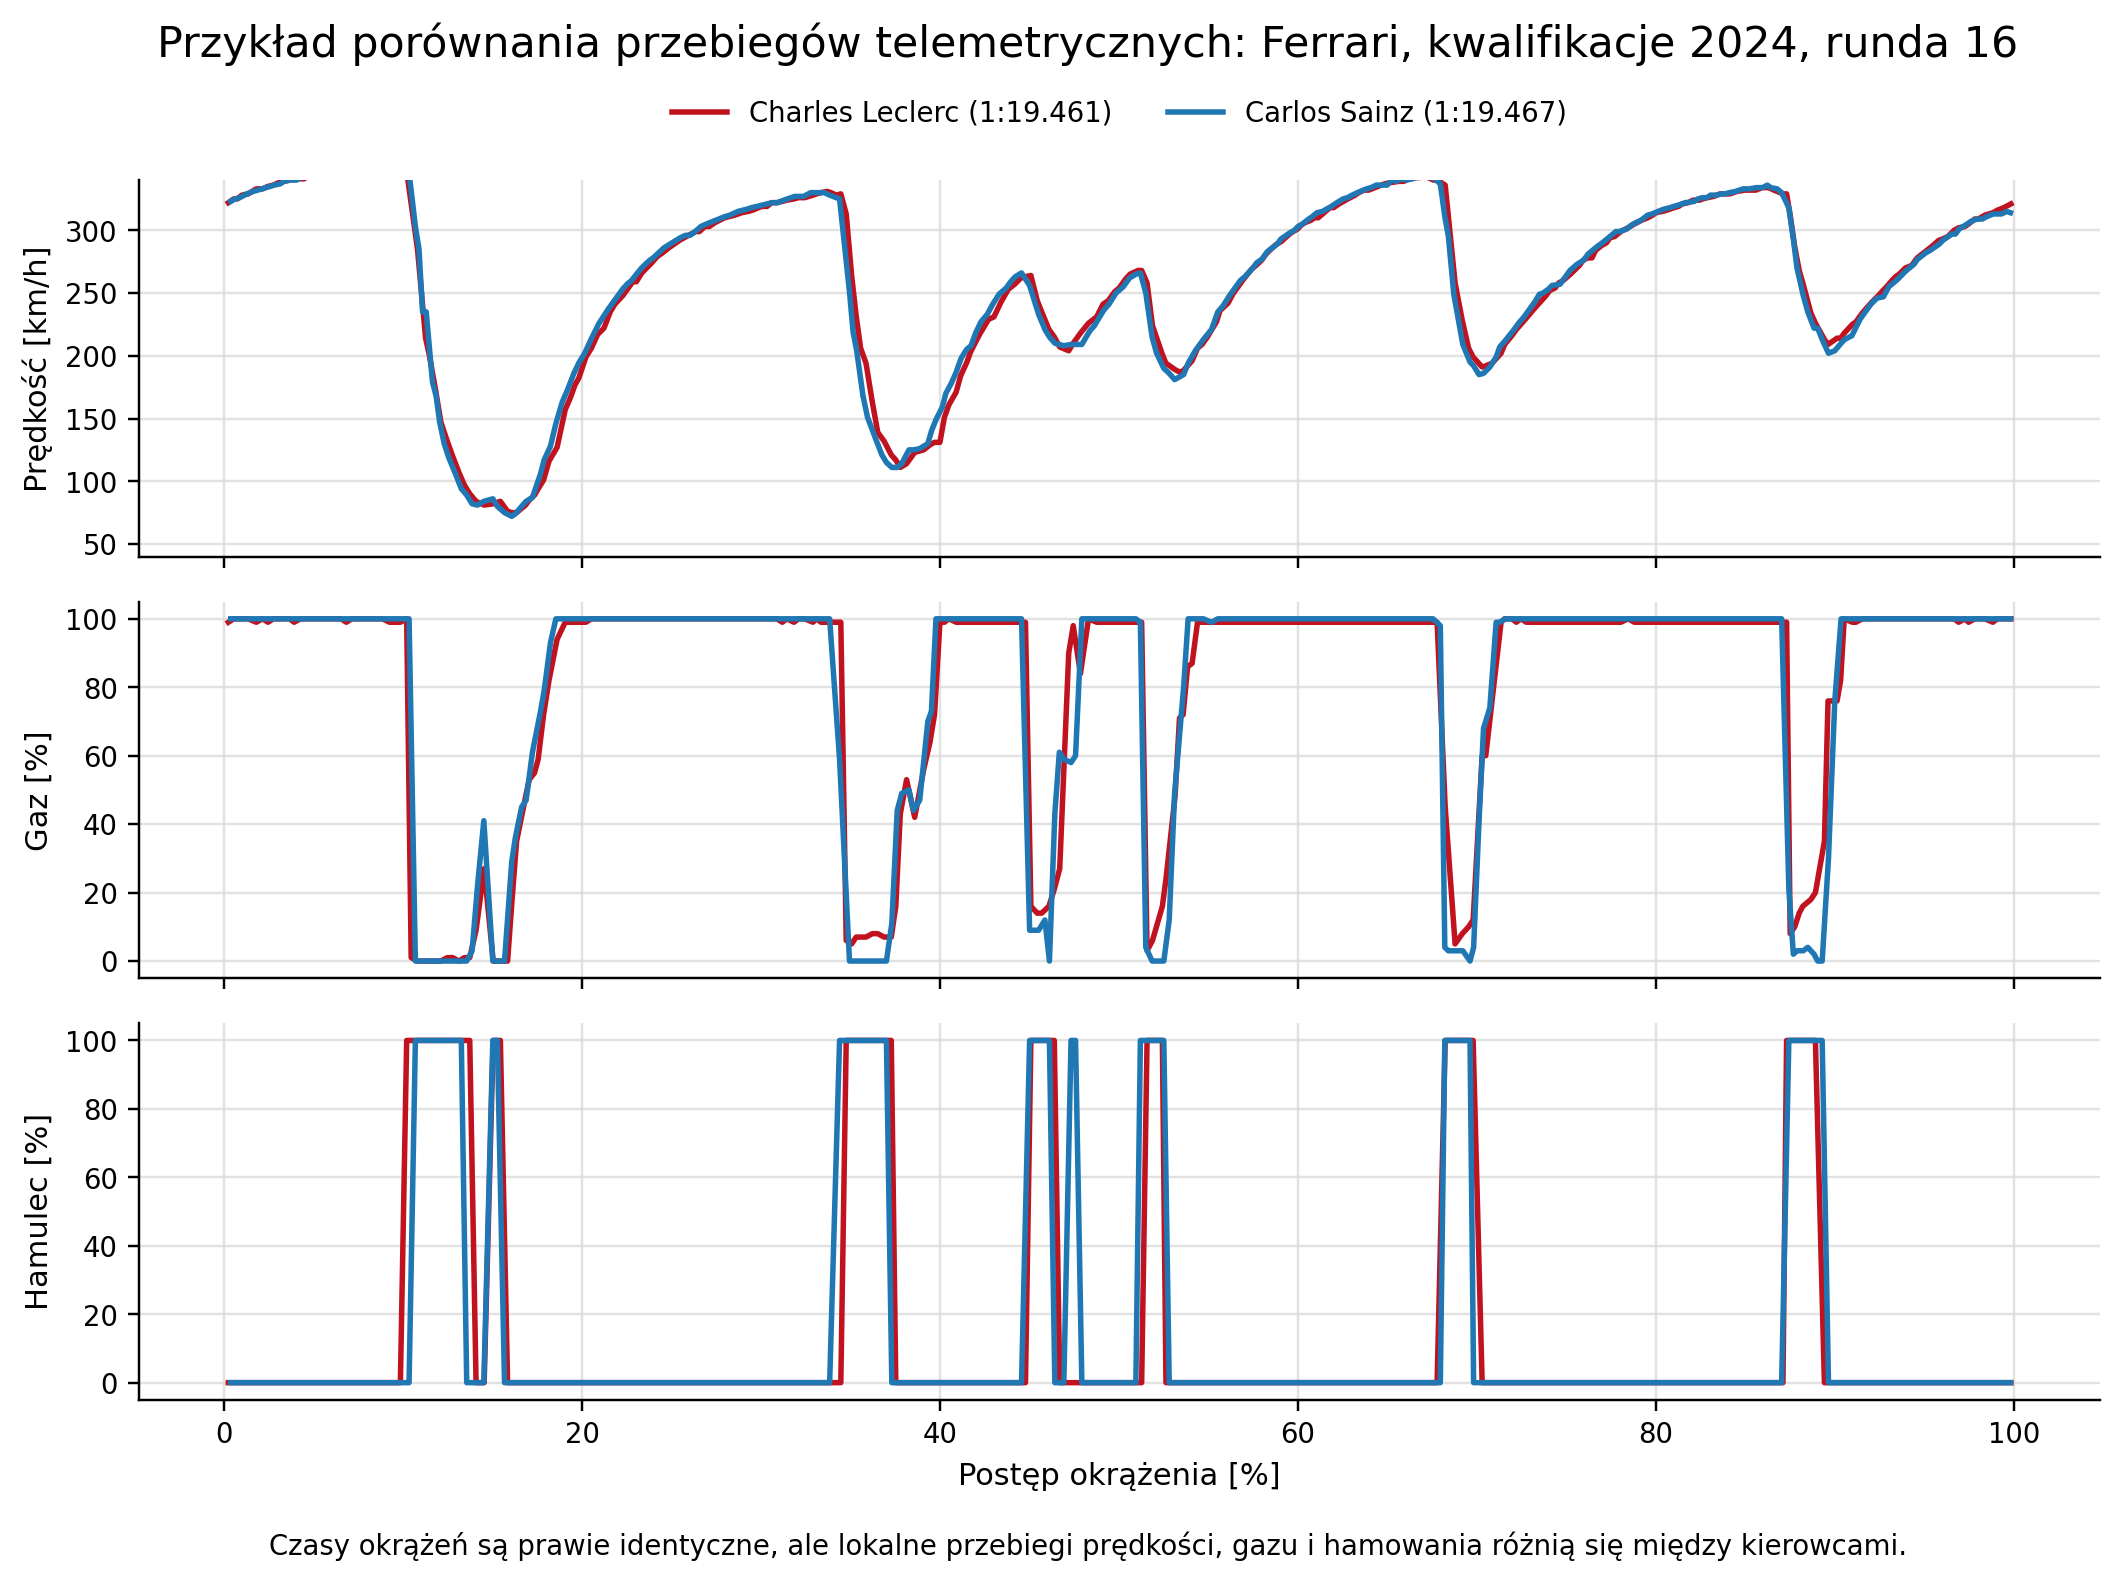
\includegraphics[width=0.9\textwidth]{figures/thesis/telemetry_overlay_lec_sai_2024_r16.png}
    \caption{Przykład porównania przebiegów telemetrycznych dla dwóch kierowców z bardzo podobnym czasem okrążenia.}
    \label{fig:telemetry_overlay_example}
\end{figure}
\FloatBarrier

Już na takim porównaniu można zauważyć różnice w sposobie prowadzenia samochodu. W wielu fragmentach przebiegi prawie się pokrywają, ale w wybranych częściach okrążenia pojawiają się przesunięcia w momencie hamowania, zejścia z gazu i ponownego otwarcia przepustnicy. Przykładowo w środkowej części okrążenia jeden z kierowców wcześniej stabilizuje gaz po fazie hamowania, podczas gdy drugi dłużej utrzymuje częściowe otwarcie przepustnicy. Podobne różnice widać przy końcowych strefach hamowania, gdzie niewielkie przesunięcia czasowe przekładają się na inny przebieg prędkości. Sam czas okrążenia nie opisuje więc w pełni sposobu jazdy. Dwa bardzo podobne rezultaty mogą być zbudowane z nieco innych decyzji dotyczących hamowania, gazu i utrzymywania prędkości.

Zakres publicznie dostępnej telemetrii nakłada istotne ograniczenia interpretacyjne. W danych brakuje części informacji, które byłyby bardzo cenne przy pełniejszym opisie zachowania samochodu, między innymi kąta skrętu kierownicy, sił działających na pedały, ustawień samochodu, danych z zawieszenia, dokładnych map silnika czy szczegółowych parametrów aerodynamicznych. Ogranicza to możliwość jednoznacznego wyjaśnienia wszystkich przyczyn obserwowanych różnic między kierowcami. Dostępny zakres danych nadal pozwala jednak analizować przebieg okrążenia, porównywać decyzje dotyczące hamowania i przyspieszania oraz sprawdzać, czy w tych przebiegach pojawiają się powtarzalne wzorce charakterystyczne dla kierowców.

\section{Styl jazdy i identyfikacja kierowcy w literaturze}

Pojęcie stylu jazdy można rozumieć jako powtarzalny sposób prowadzenia pojazdu, widoczny w decyzjach podejmowanych przez kierowcę w kolejnych fragmentach trasy. W kontekście danych telemetrycznych styl oznacza zbiór wzorców pojawiających się w czasie, między innymi sposób budowania prędkości, rozkład faz hamowania i przyspieszania, stabilność prowadzenia samochodu oraz konsekwencję podobnych decyzji w wielu przejazdach. Pozwala to potraktować styl jazdy jako problem analizy danych, a nie wyłącznie opis jakościowy.

W literaturze można znaleźć wiele prac pokazujących, że zachowanie kierowcy pozostawia mierzalny ślad w danych z pojazdu. Systemy rozpoznawania stylu jazdy i zachowania kierowców są opisywane między innymi w kontekście bezpieczeństwa, systemów wspomagania kierowcy, ubezpieczeń oraz personalizacji pojazdu \cite{driving_style_review}. Kluczowa jest tutaj sama idea, zgodnie z którą powtarzalny sposób prowadzenia pojazdu powinien częściowo ujawniać się w danych.

W pracach dotyczących identyfikacji kierowcy często wykorzystuje się dane z czujników samochodu, magistrali CAN-BUS lub systemów OBD-II. Klasyfikacja osoby prowadzącej pojazd może być oparta na sygnałach rejestrowanych przez samochód \cite{driver_can_identification}, a w wybranych podejściach nawet na danych z pojedynczego zakrętu \cite{hallac2016}. Jest to szczególnie bliskie tematyce tej pracy, ponieważ zakręt koncentruje wiele decyzji kierowcy w krótkim czasie, takich jak hamowanie, redukcja biegu, utrzymanie prędkości minimalnej i powrót na gaz.

Inny przykład stanowią badania oparte na danych telematycznych z normalnej jazdy drogowej, gdzie identyfikacja kierowcy może być łączona z analizą ważności cech, na przykład przy użyciu modelu Random Forest \cite{wang2017}. Podobne założenie przyjęto w części interpretowalnej, w której modele oparte na ręcznie zdefiniowanych cechach służą do rozpoznania kierowcy oraz wskazania cech najmocniej wpływających na decyzję modelu.

Nowsze podejścia coraz częściej wykorzystują reprezentacje ukryte i głębokie uczenie. Przykładem jest Driver2vec \cite{driver2vec}, czyli model tworzący embedding stylu jazdy na podstawie krótkiego fragmentu danych. Styl kierowcy można więc traktować jako reprezentację wydobytą automatycznie z przebiegu sygnałów, a nie wyłącznie jako zestaw ręcznie wybranych cech. Podobną logikę wykorzystują modele sekwencyjne i hybrydowe zastosowane w eksperymentach.

W kontekście Formuły 1 dostępnych prac naukowych jest mniej niż w obszarze klasycznej telematyki drogowej. Publiczne dane F1 są bogate, ale nadal ograniczone względem danych zespołowych. Pojawiają się jednak prace i projekty analizujące trajektorie telemetryczne, klasteryzację oraz identyfikację kierowcy na podstawie fragmentów zakrętów \cite{f1_fda_thesis,withseismic2026}. Temat jest więc aktualny, ale nadal pozostawia miejsce na własną analizę porównującą modele tabularne, sekwencyjne i hybrydowe oraz badającą wpływ zespołu na wyniki klasyfikacji.

Na tle tych prac analiza łączy publiczne dane Formuły 1, pełny proces od audytu danych po modele klasyfikacyjne oraz porównanie trzech setupów badawczych. Oprócz samej skuteczności klasyfikacji uwzględniono interpretowalność wyników oraz wpływ zespołu i samochodu na rozpoznawany profil telemetryczny.

\section{Klasyfikacja nadzorowana}

Problem rozpoznawania kierowcy sformułowano jako wieloklasową klasyfikację nadzorowaną. W takim zadaniu dla każdej próbki znana jest etykieta, a model uczy się odwzorowania między wejściem a klasą \cite{bishop2006}. Za etykietę przyjęto kierowcę, a wejściem był albo wektor cech opisujących całe okrążenie, albo sekwencja telemetryczna.

Najważniejszym problemem w klasyfikacji jest generalizacja, czyli działanie modelu na danych niewidzianych podczas uczenia. Wysoki wynik treningowy połączony ze słabym wynikiem walidacyjnym lub testowym oznacza przeuczenie. W analizowanym zbiorze szczególnie ważne było podobieństwo okrążeń z tej samej sesji, dlatego zastosowano walidację grupowaną po sesjach.

\section{Regresja logistyczna}

Regresja logistyczna jest jednym z podstawowych modeli klasyfikacyjnych. Pomimo nazwy odnoszącej się do regresji, w tym zastosowaniu model estymuje prawdopodobieństwo przynależności próbki do danej klasy \cite{bishop2006}. Najpierw tworzona jest liniowa kombinacja cech, a następnie wynik zostaje przekształcony do przedziału od 0 do 1 za pomocą funkcji logistycznej.

Dla przypadku binarnego funkcję logistyczną można zapisać jako:

\[
\sigma(z) = \frac{1}{1 + e^{-z}},
\]

gdzie \(z\) jest wynikiem liniowym modelu. W klasyfikacji wieloklasowej stosuje się analogiczne podejście z funkcją softmax, która zwraca rozkład prawdopodobieństwa po klasach.

\begin{figure}[H]
\centering
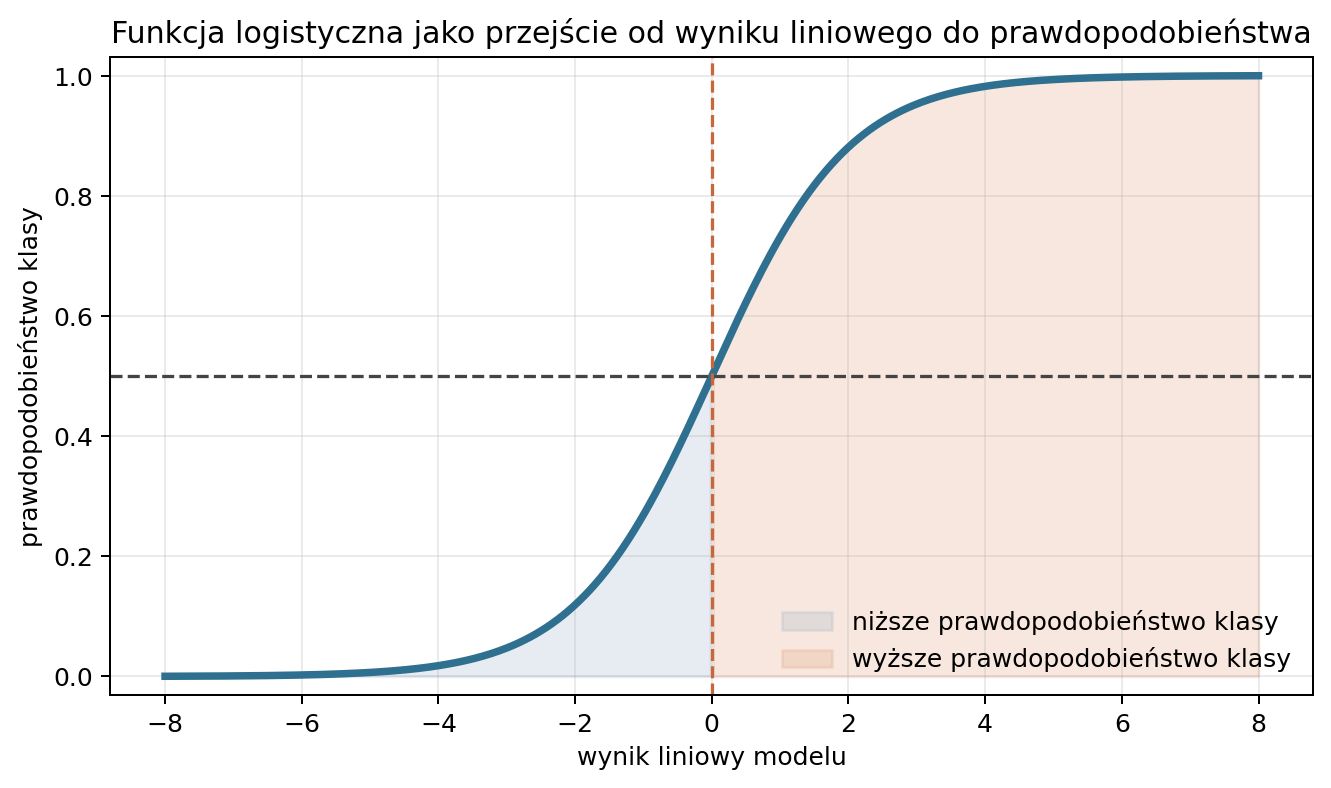
\includegraphics[width=0.64\textwidth]{30_theory_logistic_sigmoid.png}
\caption{Funkcja logistyczna jako przejście od wyniku liniowego do prawdopodobieństwa.}
\label{fig:theory-logistic}
\end{figure}
\FloatBarrier

Regresja logistyczna pełni rolę modelu interpretowalnego. Poza samą klasyfikacją pozwala analizować cechy na podstawie wartości współczynników. Jeżeli dana cecha ma duży współczynnik dla konkretnej klasy, jej większa wartość zwiększa prawdopodobieństwo przypisania próbki do tej klasy. Współczynniki wskazują, które cechy telemetryczne model uznał za przydatne; interpretacja przyczynowa wymaga jednak dodatkowej ostrożności.

W modelach liniowych ważna jest regularyzacja, czyli dodatkowe ograniczenie nakładane na wartości parametrów modelu podczas uczenia \cite{bishop2006}. Można ją rozumieć jako sposób zmniejszenia ryzyka zbyt mocnego dopasowania modelu do danych treningowych. Regularyzacja L2 ogranicza zbyt duże wartości współczynników, a regularyzacja L1 może dodatkowo prowadzić do wyzerowania części z nich. Ma to znaczenie zwłaszcza przy dużej liczbie cech i potrzebie uzyskania prostszego, bardziej stabilnego modelu.

\section{Modele drzewiaste i boostingowe}

Modele drzewiaste dzielą przestrzeń cech na prostsze obszary decyzyjne. Pojedyncze drzewo decyzyjne jest łatwe do zrozumienia, ale może łatwo dopasować się zbyt mocno do danych treningowych. Random Forest ogranicza ten problem przez budowę wielu drzew na losowych podzbiorach danych i cech, a następnie agregację ich predykcji \cite{breiman2001}.

Modele boostingowe budują kolejne słabsze modele tak, aby poprawiały błędy poprzednich. Często osiągają bardzo dobre wyniki na danych tabularnych, wymagając przy tym kontroli przeuczenia. Random Forest, HistGradientBoosting oraz XGBoost potraktowano jako modele porównawcze dla podejść liniowych i sekwencyjnych.

Różnicę między podejściem typu Random Forest a boostingiem przedstawiono schematycznie na rysunku~\ref{fig:theory-tree-boosting}. W pierwszym przypadku wiele drzew powstaje równolegle, a wynik jest agregowany. W drugim kolejne drzewa są dodawane sekwencyjnie i skupiają się na poprawianiu błędów wcześniejszych modeli.

\begin{figure}[H]
\centering
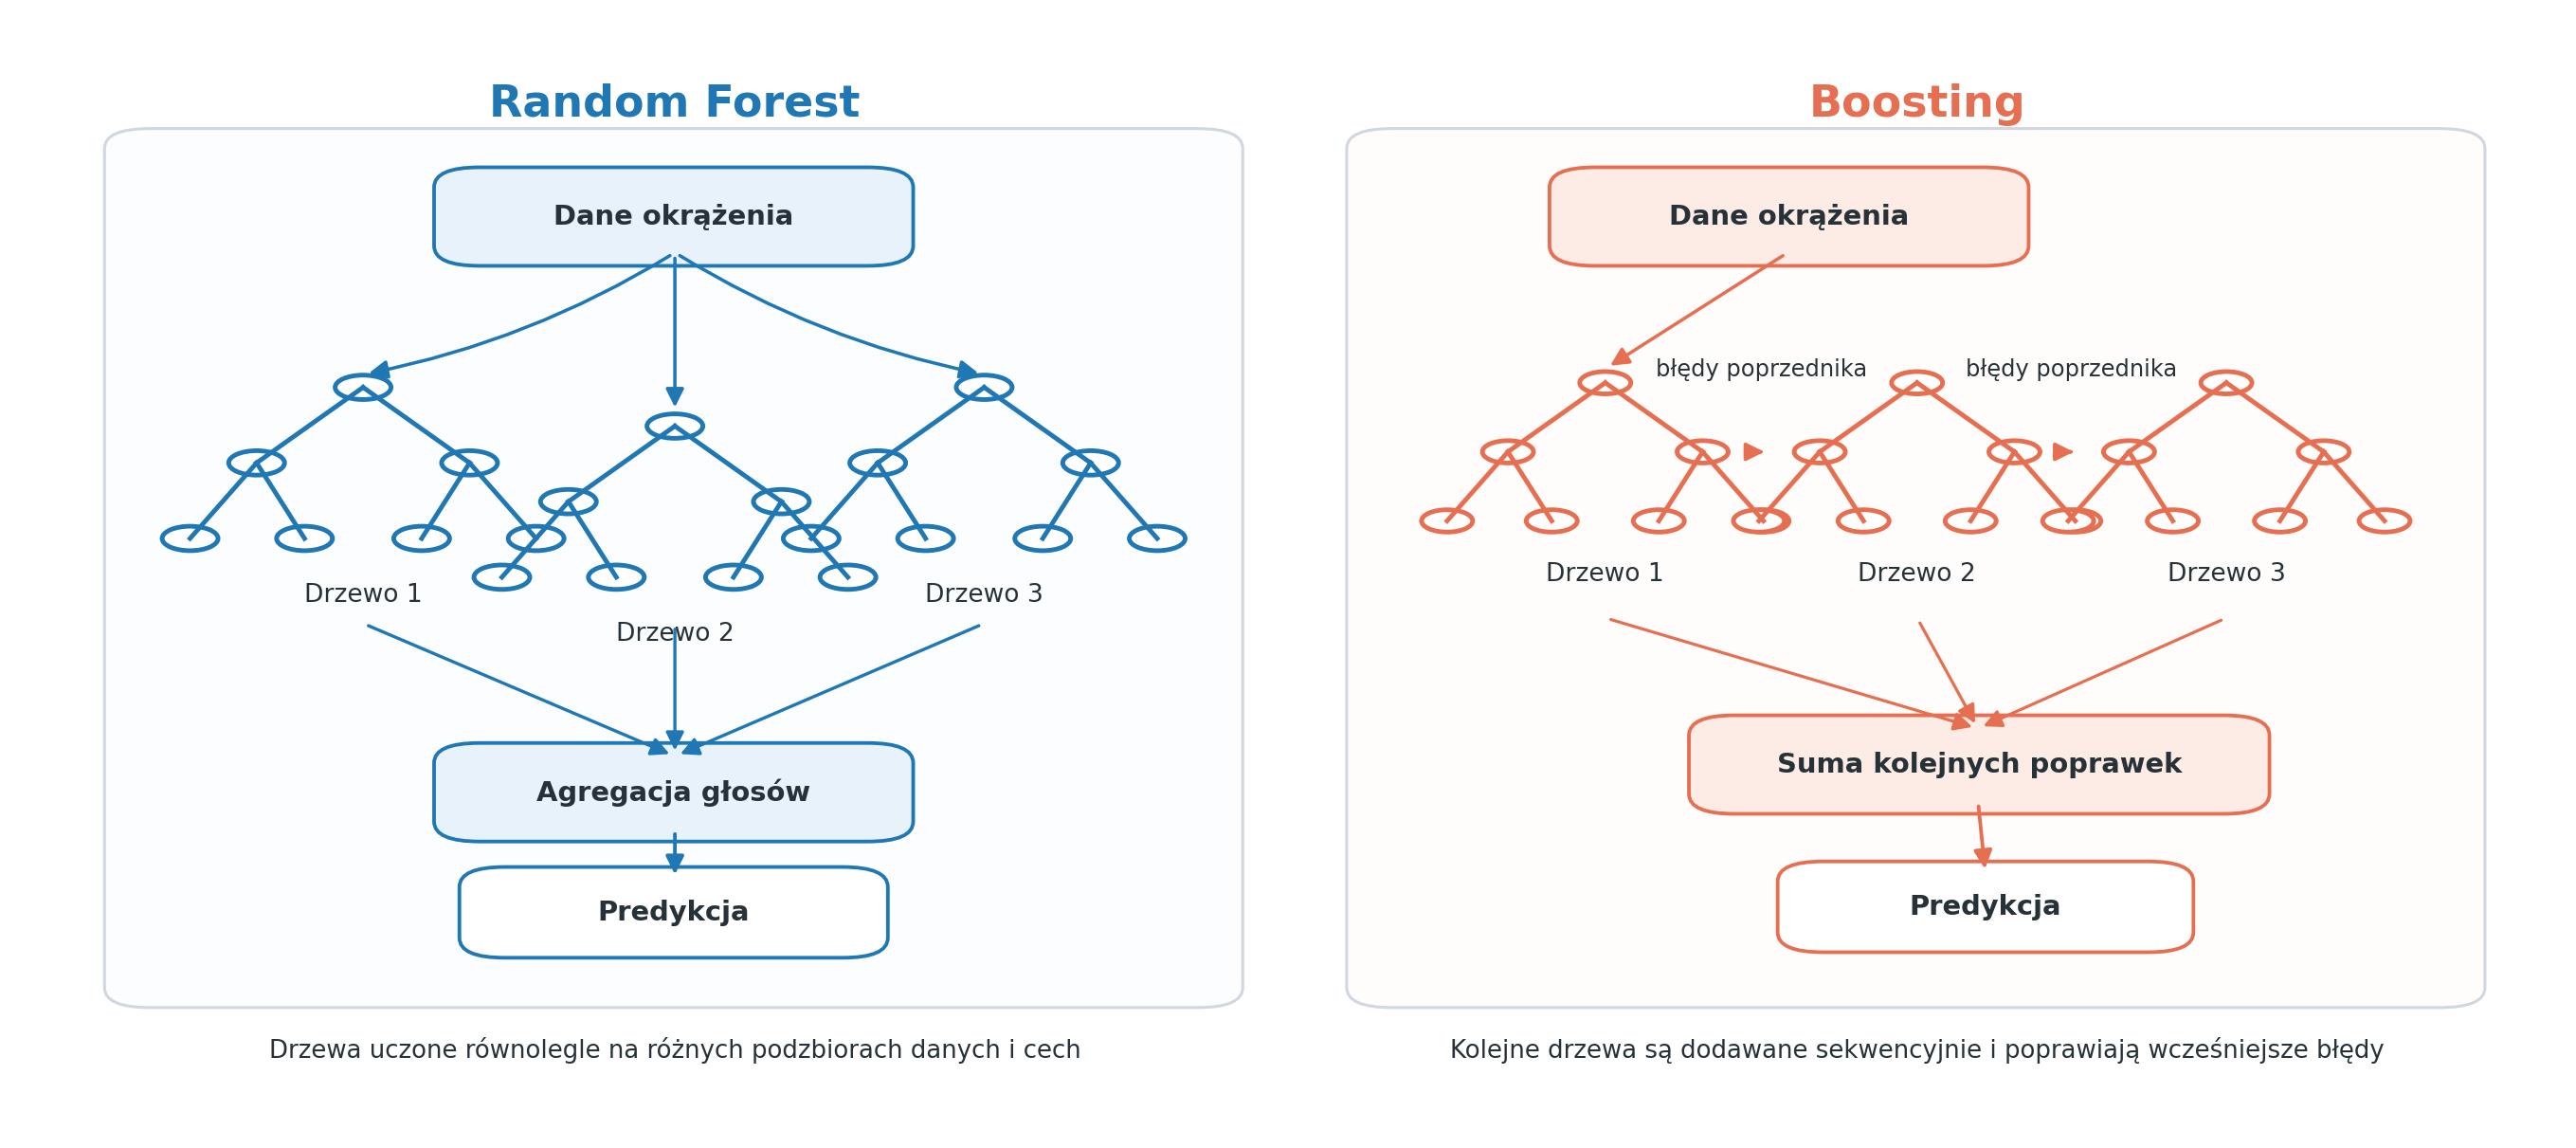
\includegraphics[width=0.98\textwidth,height=0.30\textheight,keepaspectratio=false]{33_theory_tree_boosting_concept.png}
\caption{Schematyczne porównanie idei Random Forest i modeli boostingowych.}
\label{fig:theory-tree-boosting}
\end{figure}
\FloatBarrier

\section{Modele sekwencyjne i CNN 1D}

Okrążenie Formuły 1 jest naturalnym szeregiem czasowym. Kolejne punkty telemetrii opisują, jak zmieniają się prędkość, gaz, hamowanie, obroty i bieg w trakcie przejazdu. Zamiast sprowadzać taki przebieg wyłącznie do kilku statystyk, można przekazać modelowi całą sekwencję sygnałów. Aby było to możliwe w sieci neuronowej, okrążenia o różnej liczbie próbek zostały przeskalowane do tej samej długości.

Sieć konwolucyjna 1D (\texttt{1D CNN}) przesuwa filtry po osi czasu i szuka lokalnych wzorców. W przypadku telemetrii takim wzorcem może być fragment hamowania, przejście z hamowania do gazu, stabilizacja prędkości albo seria zmian biegów. Klasyczne sieci konwolucyjne są znane głównie z analizy obrazów, a idea lokalnego filtra może być stosowana również do sygnałów jednowymiarowych \cite{lecun1998}.

\begin{figure}[H]
\centering
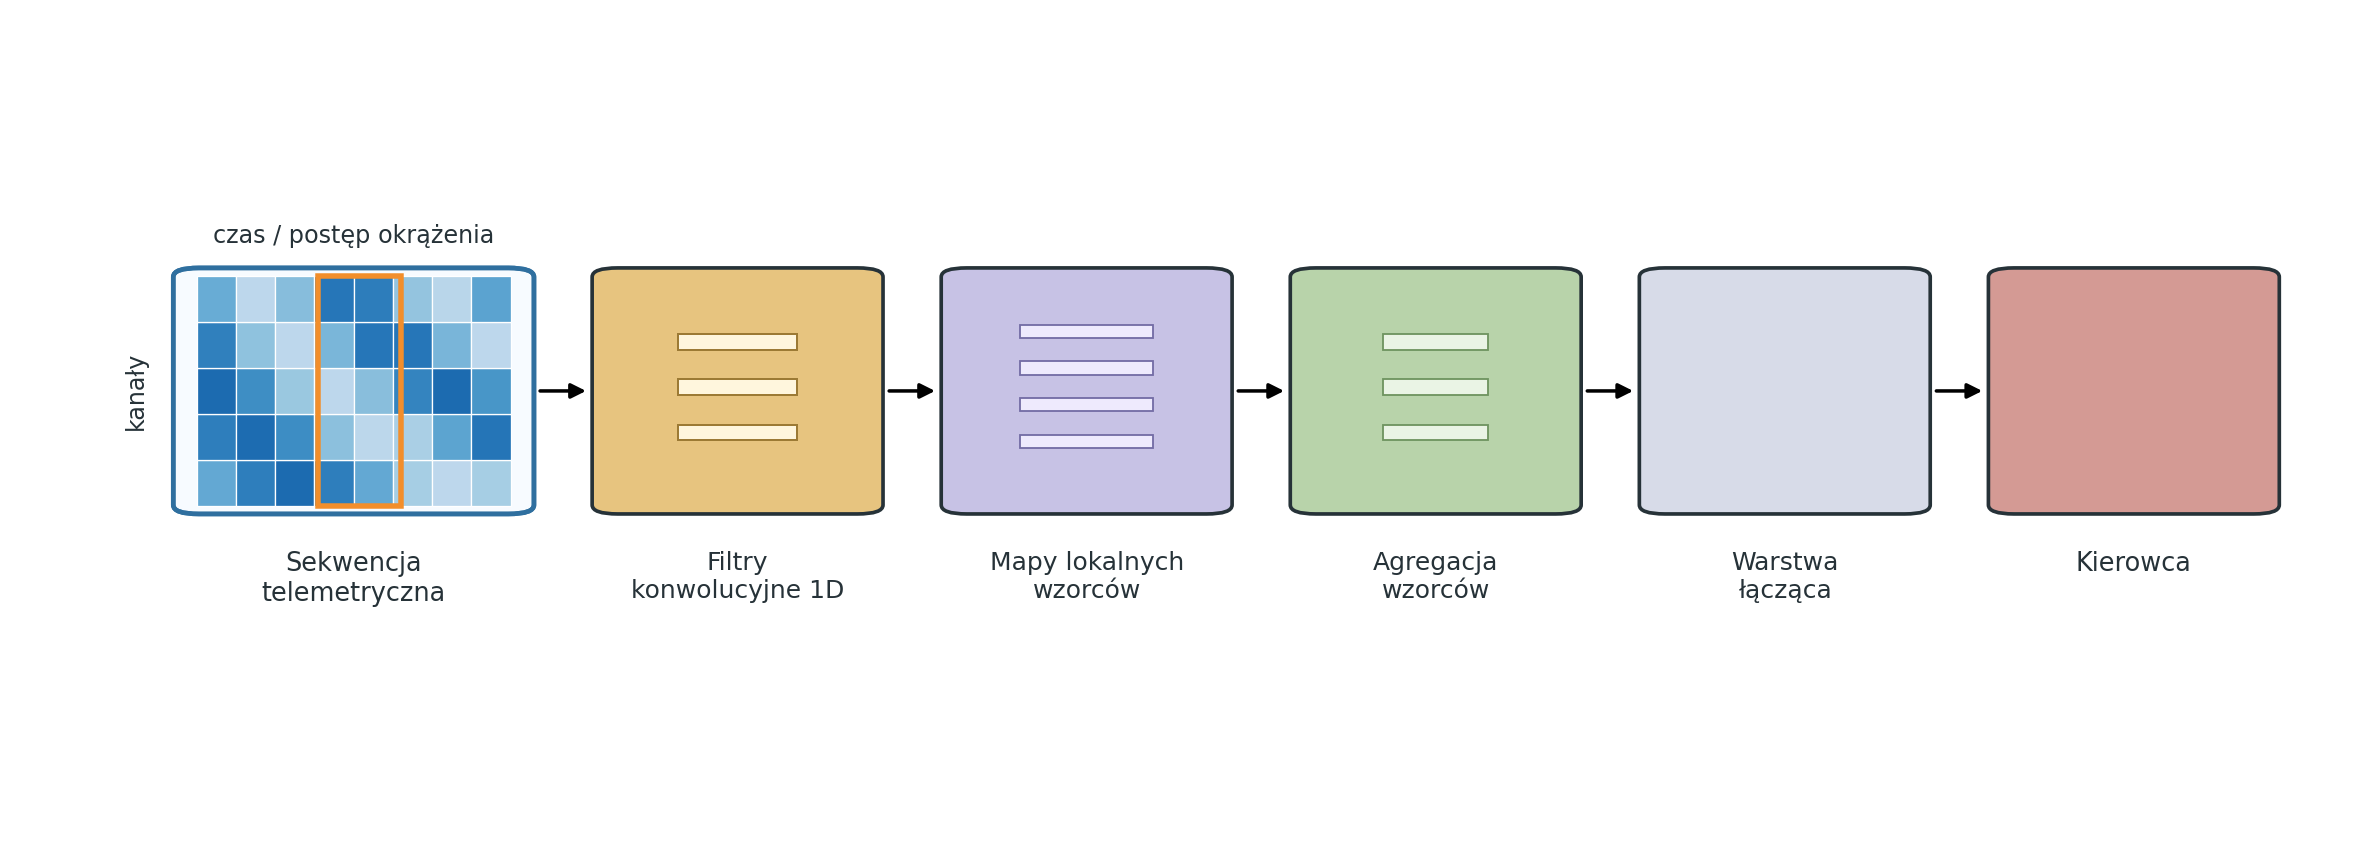
\includegraphics[width=\textwidth]{31_theory_1d_cnn_concept.png}
\caption{Schemat działania modelu CNN 1D dla sekwencji telemetrycznej.}
\label{fig:theory-cnn}
\end{figure}
\FloatBarrier

\texttt{CNN} dobrze pasuje do tego problemu, ponieważ styl jazdy może ujawniać się w krótkich fragmentach okrążenia. Model nie musi znać ręcznie opisanych zakrętów, aby wykrywać powtarzalne lokalne wzorce w przebiegu sygnałów.

\section{GRU, LSTM i model hybrydowy}

Modele rekurencyjne analizują sekwencję krok po kroku, przenosząc informację o wcześniejszych elementach sygnału. Klasyczne sieci rekurencyjne mają jednak problem z uczeniem długich zależności, dlatego opracowano architektury z bramkami, takie jak \texttt{LSTM} i \texttt{GRU}. \texttt{LSTM} wykorzystuje mechanizm komórki pamięci i bramek, aby łatwiej przechowywać informacje przez dłuższy czas \cite{hochreiter1997}. \texttt{GRU} jest uproszczoną architekturą bramkową również zaprojektowaną do pracy z sekwencjami \cite{cho2014}.

W analizowanym problemie sprawdzono \texttt{GRU} i \texttt{LSTM}, ponieważ okrążenie jest naturalnie uporządkowanym przebiegiem czasowym. Architektury rekurencyjne stanowią naturalny punkt porównania dla \texttt{CNN}. Mocniej akcentują zależności rozwijające się w czasie, podczas gdy konwolucje dobrze obrazują lokalne wzorce w krótszych fragmentach sekwencji.

Ostatnim wariantem był model hybrydowy. Łączy on reprezentację sekwencyjną z cechami tabularnymi, dzięki czemu wykorzystuje lokalne wzorce telemetrii oraz syntetyczne informacje o całym okrążeniu, np. średnią prędkość, udział pełnego gazu czy liczbę zmian biegów.

\section{Nowoczesne podejścia do klasyfikacji szeregów czasowych}

Klasyfikacja szeregów czasowych jest osobnym obszarem uczenia maszynowego, w którym porównuje się metody oparte na odległościach, kształtach fragmentów sygnału, cechach transformowanych oraz modelach głębokich \cite{bagnall2017_bakeoff,middlehurst2024_bakeoffredux}. W tym kontekście okrążenie Formuły 1 można traktować jako wielowymiarowy szereg czasowy, gdzie kanały telemetryczne opisują przebieg jazdy w kolejnych punktach okrążenia. Taka reprezentacja uwzględnia średnie i maksymalne wartości sygnałów, a także kolejność zdarzeń oraz lokalny kształt przebiegu.

Przeglądy głębokiego uczenia dla klasyfikacji szeregów czasowych pokazują, że silną rodziną modeli są architektury konwolucyjne, w tym warianty inspirowane sieciami typu Inception \cite{fawaz2019_tsc_review,inceptiontime2019}. Z takim kierunkiem dobrze korespondują wyniki uzyskane w części badawczej, gdzie najlepsze rezultaty osiągały modele \texttt{CNN} i hybrydowe. Naturalnym kierunkiem rozbudowy modeli sekwencyjnych są Temporal Convolutional Networks, które wykorzystują przyczynowe i rozszerzane konwolucje do modelowania dłuższych zależności sekwencyjnych \cite{bai2018_tcn}.

W nowszych pracach coraz częściej pojawiają się również transformery oraz uczenie reprezentacji szeregów czasowych. Modele takie jak Informer czy PatchTST pokazują, że mechanizmy uwagi i tokenizacja fragmentów szeregu mogą być stosowane do danych czasowych \cite{informer2021,patchtst2023}. Równolegle rozwijane są metody samonadzorowanego i kontrastywnego uczenia reprezentacji, między innymi TS2Vec oraz TS-TCC \cite{ts2vec2022,tstcc2021,ssl_timeseries_survey2023}. Podobnie jak wcześniej wspomniany Driver2vec, metody te prowadzą do tworzenia wektorowych reprezentacji zachowania w szerszym kontekście klasyfikacji i reprezentacji szeregów czasowych. Dla telemetrii wyścigowej takie podejścia są interesujące, ponieważ mogłyby tworzyć embeddingi stylu jazdy bez ręcznego definiowania wszystkich cech. Część eksperymentalna skupia się na bardziej kontrolowalnym porównaniu regresji logistycznej, \texttt{CNN}, \texttt{GRU}, \texttt{LSTM} i modelu hybrydowego, a nowsze architektury pozostają kierunkiem dalszych badań.

\section{Walidacja i metryki}

W klasyfikacji najprostszy podział na trening i test może prowadzić do zbyt optymistycznych wyników, szczególnie gdy próbki są naturalnie pogrupowane. Grupą przyjętą w walidacji była sesja. Okrążenia z jednej sesji mają ten sam tor, warunki i podobny kontekst, dlatego nie powinny trafiać jednocześnie do treningu i testu.

Główną metodą walidacji był \texttt{StratifiedGroupKFold}, czyli wariant walidacji krzyżowej łączący zachowanie podobnych proporcji klas w foldach z rozdzieleniem grup między trening i test \cite{sklearn_sgkf}.

\begin{figure}[H]
\centering
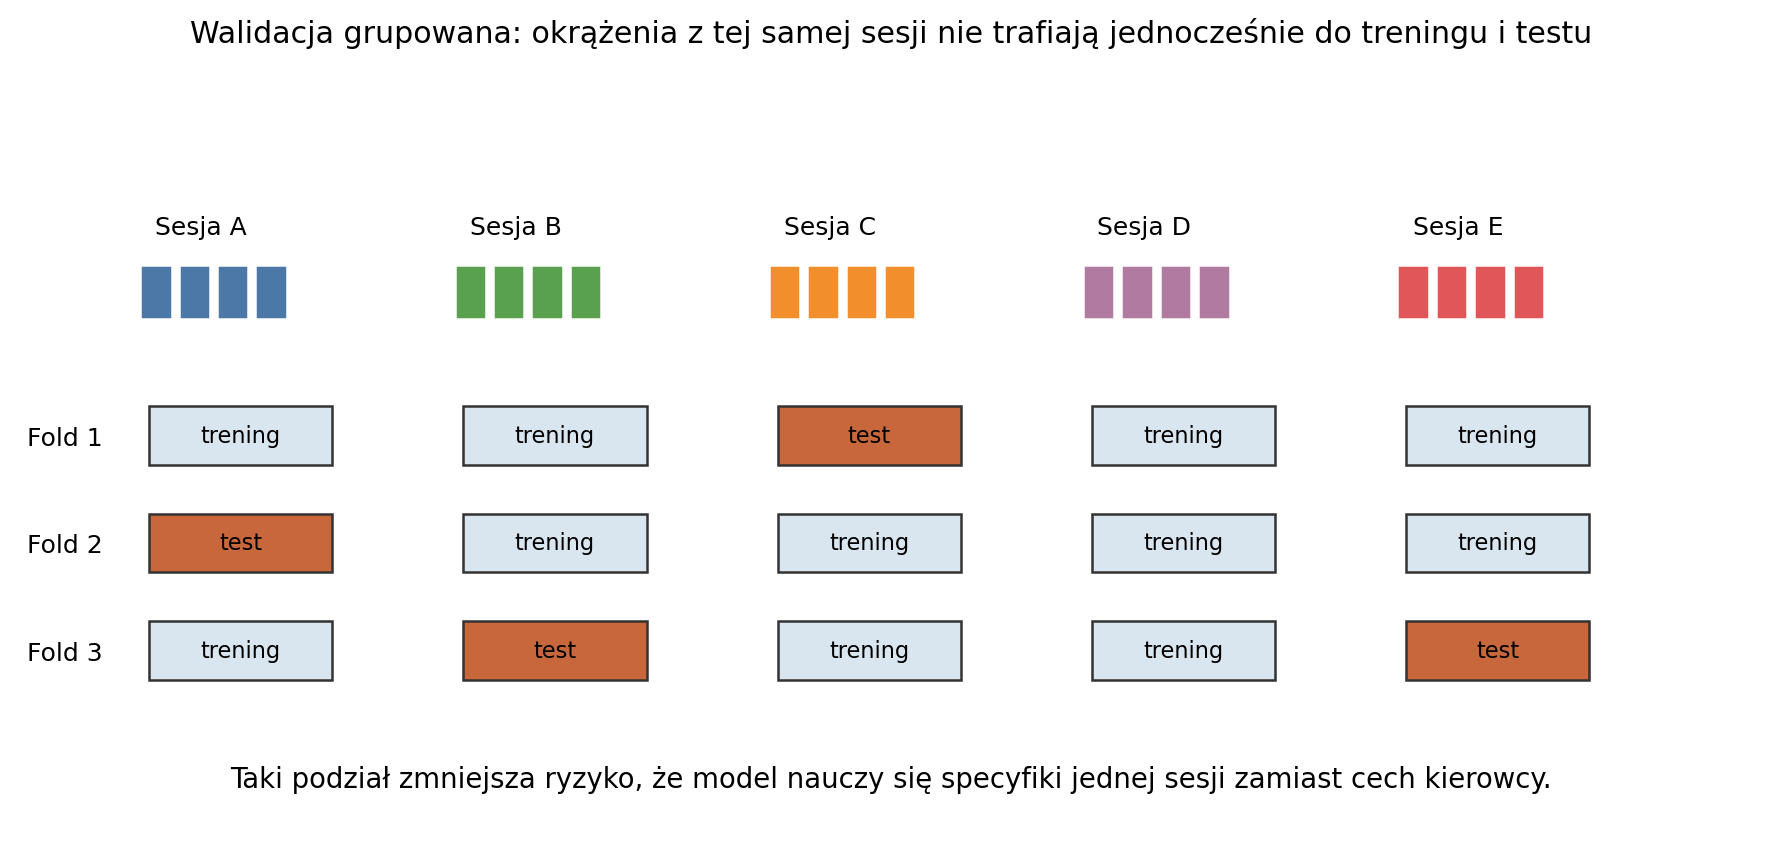
\includegraphics[width=0.90\textwidth]{32_theory_grouped_cv.png}
\caption{Schemat walidacji grupowanej po sesjach.}
\label{fig:theory-grouped-cv}
\end{figure}
\FloatBarrier

Do oceny modeli użyto kilku metryk. Accuracy oznacza udział poprawnych predykcji:

\[
Accuracy = \frac{\text{liczba poprawnych predykcji}}{\text{liczba wszystkich predykcji}}.
\]

Sama accuracy może jednak być myląca, jeżeli klasy są nierówno reprezentowane. Dlatego za główną metrykę przyjęto macro F1. Dla każdej klasy liczone są precision i recall, następnie F1:

\[
F1 = 2 \cdot \frac{precision \cdot recall}{precision + recall}.
\]

Macro F1 jest średnią wartości F1 po klasach. Metryka ta pozwala oceniać jakość modeli w problemach wieloklasowych bez nadmiernego faworyzowania najliczniejszych klas \cite{sokolova2009}. W analizie kierowców jest szczególnie użyteczna, ponieważ każda klasa ma podobne znaczenie w końcowym wyniku, niezależnie od liczby okrążeń danego kierowcy. Dodatkowo analizowano macierze pomyłek, pokazujące ogólny wynik oraz pary kierowców najczęściej mylone przez model.

\chapter{Dane i eksploracyjna analiza danych}

\section{Źródła danych}

Podstawowym źródłem danych była biblioteka \texttt{FastF1}. Jest to biblioteka Pythona przeznaczona do pobierania i analizy publicznie dostępnych danych Formuły 1. Jej najważniejszą zaletą w tym projekcie była możliwość połączenia kilku typów informacji w jednym procesie przetwarzania danych, obejmującym czasy okrążeń, sektory, informacje o oponach, wyniki sesji, dane pogodowe, telemetrię samochodu, dane pozycyjne oraz harmonogram wydarzeń. Biblioteka udostępnia między innymi dane okrążeń, telemetrię samochodu, pozycję, dane opon, pogodę, harmonogram sesji oraz wyniki \cite{fastf1_docs}.

Najczęściej wykorzystywanym obiektem była sesja, np. kwalifikacje albo wyścig dla konkretnego Grand Prix. Po załadowaniu sesji można uzyskać tabelę okrążeń, wyniki, dane pogodowe oraz przebiegi telemetryczne dla wybranych kierowców i okrążeń. Tabela okrążeń zawierała między innymi kierowcę, numer okrążenia, czas okrążenia, czasy sektorów, mieszankę opon, wiek opon, status toru oraz informację o poprawności okrążenia. Dane telemetryczne obejmowały sygnały takie jak \texttt{Speed}, \texttt{Throttle}, \texttt{Brake}, \texttt{RPM}, \texttt{nGear}, \texttt{DRS}, a dane pozycyjne pozwalały uzyskać współrzędne \texttt{X}, \texttt{Y}, \texttt{Z}.

Biblioteka była szczególnie wygodna w tym projekcie, ponieważ umożliwiała przejście od poziomu sesji do poziomu pojedynczego okrążenia. Proces rozpoczęto od audytu dostępności danych i filtrowania okrążeń według warunków oraz jakości. Telemetrię pobierano już dla wybranych próbek, co miało znaczenie praktyczne. Pobieranie pełnych przebiegów telemetrycznych dla wszystkich okrążeń jest dużo bardziej czasochłonne niż praca na tabelach okrążeń.

\texttt{FastF1} korzysta z danych pobieranych z zewnętrznych źródeł, dlatego istotne było użycie lokalnego cache. Pozostawienie cache włączonego przyspiesza ponowne uruchamianie skryptów i pomaga uniknąć przekraczania limitów serwerów API \cite{fastf1_docs}. Pierwsze pobranie sesji mogło trwać długo, natomiast kolejne uruchomienia korzystały już z danych zapisanych lokalnie. Przy pobieraniu wielu sezonów ograniczało to czas działania skryptów i liczbę ponownych zapytań do tych samych endpointów.

Zakres danych udostępnianych przez \texttt{FastF1} jest węższy niż zakres danych inżynierskich dostępnych zespołom Formuły 1. Ogranicza to możliwość pełnego wyjaśniania przyczyn obserwowanych różnic, choć nadal pozwala badać te elementy stylu jazdy, które są widoczne w publicznym przebiegu okrążenia.

Pomocniczo rozważano również źródła takie jak Jolpica oraz OpenF1. Jolpica jest istotna przede wszystkim jako źródło metadanych i następca Ergast API w ekosystemie \texttt{FastF1} \cite{fastf1_docs}. OpenF1 może być natomiast użyteczne jako dodatkowe źródło walidacji w przyszłości. W obecnym etapie głównym źródłem danych pozostało jednak \texttt{FastF1}, aby zachować spójność całego procesu pobierania, filtrowania i ekstrakcji telemetrii.

\section{Zakres danych}

W projekcie przygotowano trzy główne setupy eksperymentalne przedstawione w tabeli~\ref{tab:setups}. Każdy z nich pełni inną funkcję w analizie. Kwalifikacje 2023--2025 są najmniejszym i najczystszym punktem startowym. Kwalifikacje 2018--2025 sprawdzają, czy wniosek utrzymuje się w dłuższym horyzoncie czasowym. Czyste okrążenia wyścigowe 2025 zwiększają liczbę próbek, wprowadzając przy tym większą zmienność wynikającą z opon, paliwa, stintu i kontekstu wyścigowego.

\begin{table}[H]
\centering
\small
\begin{tabular}{l c l r}
\toprule
Setup & Zakres lat & Kierowcy & Liczba okrążeń \\
\midrule
Kwalifikacje, krótki horyzont & 2023--2025 & ALB, SAI, VER, OCO, LEC & 273 \\
Kwalifikacje, długi horyzont & 2018--2025 & SAI, VER, LEC, OCO, HAM & 698 \\
Wyścigi, czyste okrążenia & 2025 & SAI, VER, LEC, OCO, HAM & 4334 \\
\bottomrule
\end{tabular}
\caption{Główne setupy eksperymentalne.}
\label{tab:setups}
\end{table}

\begin{figure}[H]
\centering
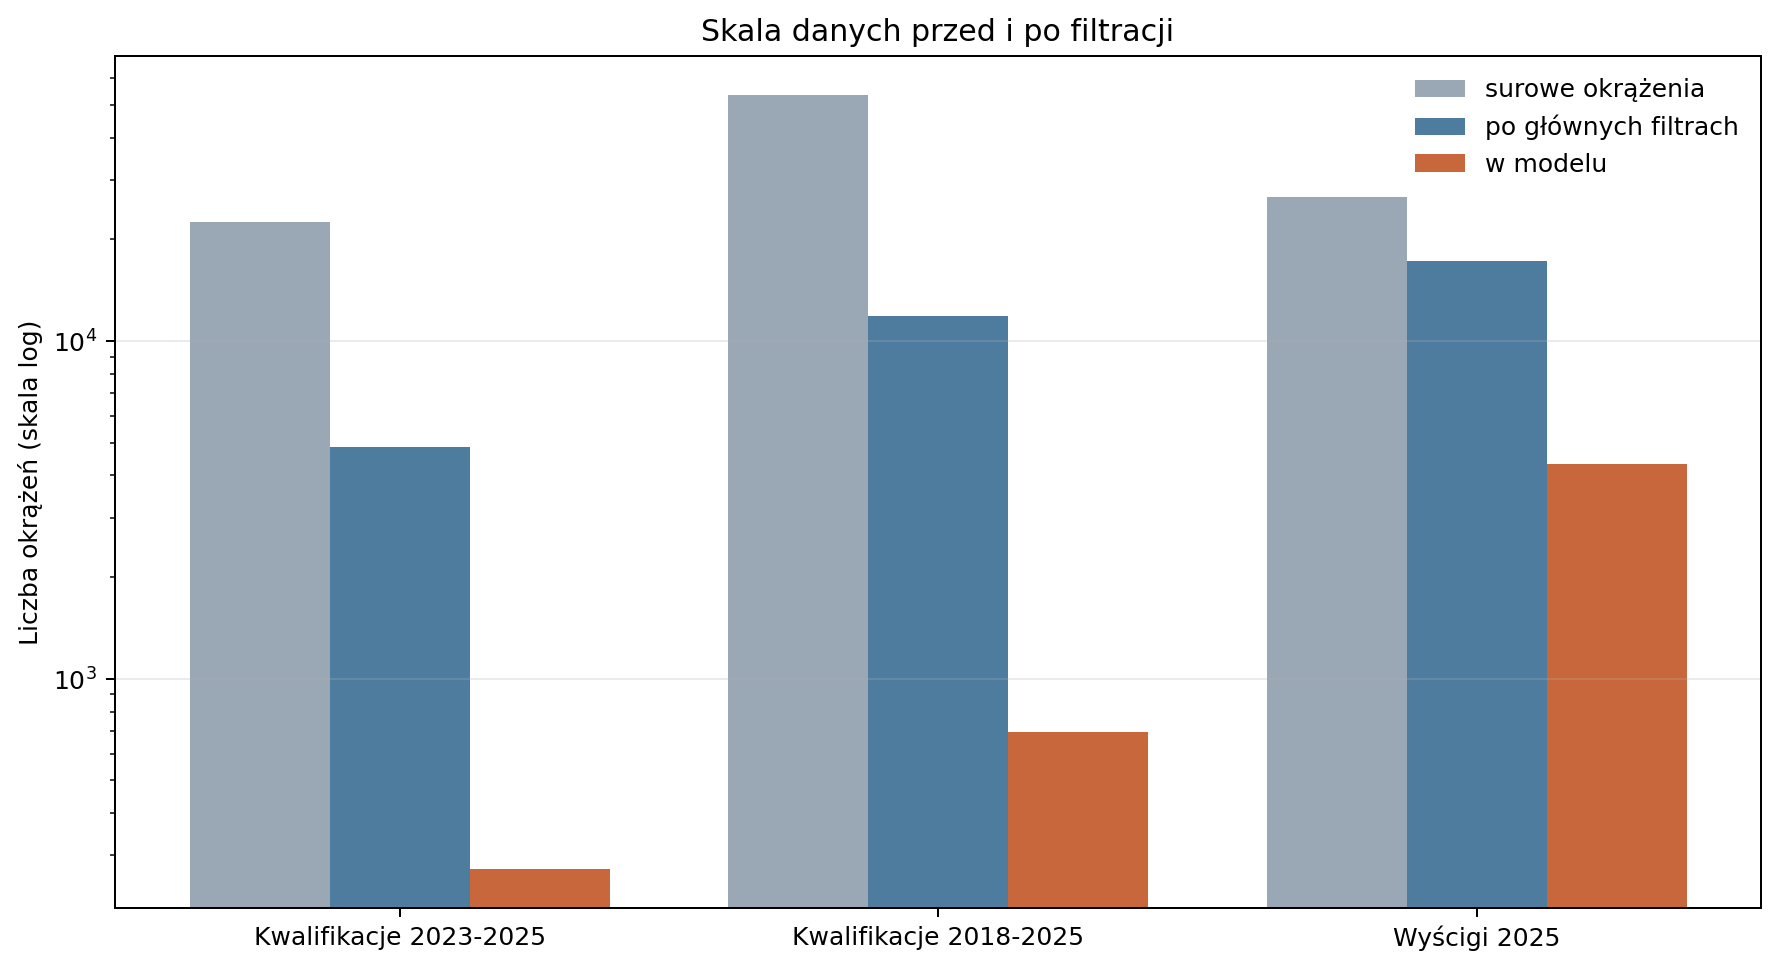
\includegraphics[width=0.95\textwidth]{24_eda_dataset_sizes.png}
\caption{Porównanie liczby okrążeń w danych surowych, po filtracji i w finalnych setupach modelowych.}
\label{fig:eda-dataset-sizes}
\end{figure}

\section{Redukcja danych}

Dane redukowano etapowo, aby uzyskać zbiór okrążeń możliwie reprezentatywnych dla analizy stylu jazdy. Filtry miały ograniczyć wpływ okrążeń nieporównywalnych, na przykład przejazdów bez poprawnego czasu, sesji mokrych, neutralizacji, zjazdów do alei serwisowej albo okrążeń odstających od normalnego tempa stintu.

W kwalifikacjach 2023--2025 punkt startowy obejmował 22465 okrążeń. Po usunięciu okrążeń bez czasu, ograniczeniu do suchych sesji, filtrze poprawności, zielonym statusie toru i wyborze personal best pozostało 4853 okrążeń w czystym zbiorze pośrednim. Finalny setup pięciu kierowców zawierał 273 okrążenia.

W kwalifikacjach 2018--2025 punkt startowy obejmował 53690 okrążeń. Po analogicznych filtrach pozostało 11848 okrążeń personal best, a finalny setup pięciu kierowców zawierał 698 okrążeń.

W wyścigach 2025 punkt startowy obejmował 26692 okrążenia. Po usunięciu okrążeń bez czasu, mokrych sesji, okrążeń niedokładnych, neutralizacji, pit-in/pit-out oraz okrążeń odstających od lokalnej mediany stintu pozostało 17265 czystych okrążeń wyścigowych. Finalny setup pięciu kierowców zawierał 4334 okrążenia.

\section{Filtrowanie danych}

Dane filtrowano etapowo. W kwalifikacjach brano pod uwagę okrążenia z poprawnym czasem, suche warunki, poprawność przejazdu, zielony status toru oraz wybór reprezentatywnego okrążenia kierowcy w sesji. Celem było pozostawienie przejazdów wykonanych w warunkach możliwie zbliżonych do normalnego szybkiego okrążenia. W wyścigach dodatkowo odrzucano okrążenia pit-in/pit-out i okrążenia odstające od lokalnej mediany stintu, aby ograniczyć wpływ zdarzeń strategicznych, błędów oraz nietypowego tempa.

\begin{figure}[H]
\centering
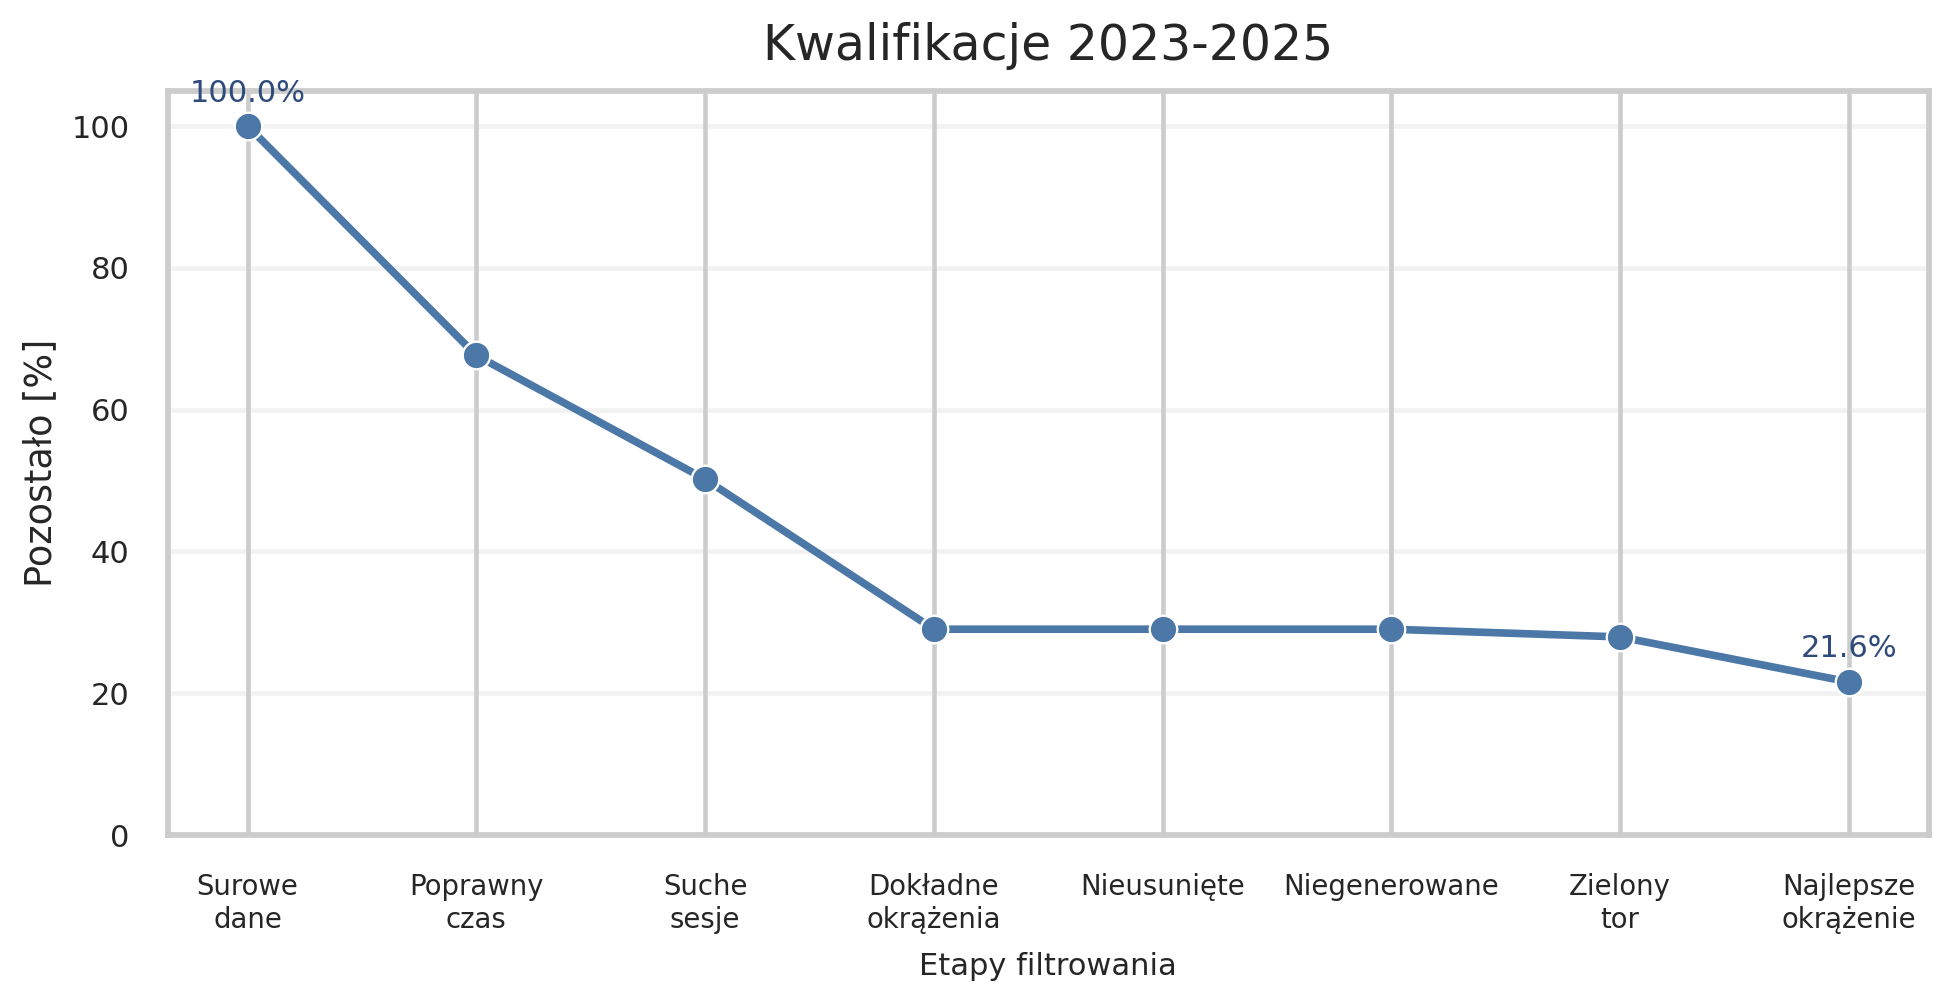
\includegraphics[width=0.92\textwidth]{01a_filter_funnel_qualifying_2023_2025.png}
\caption{Redukcja danych po kolejnych filtrach w setupie kwalifikacyjnym 2023--2025.}
\label{fig:filter-funnel-short-qualifying}
\end{figure}

\begin{figure}[H]
\centering
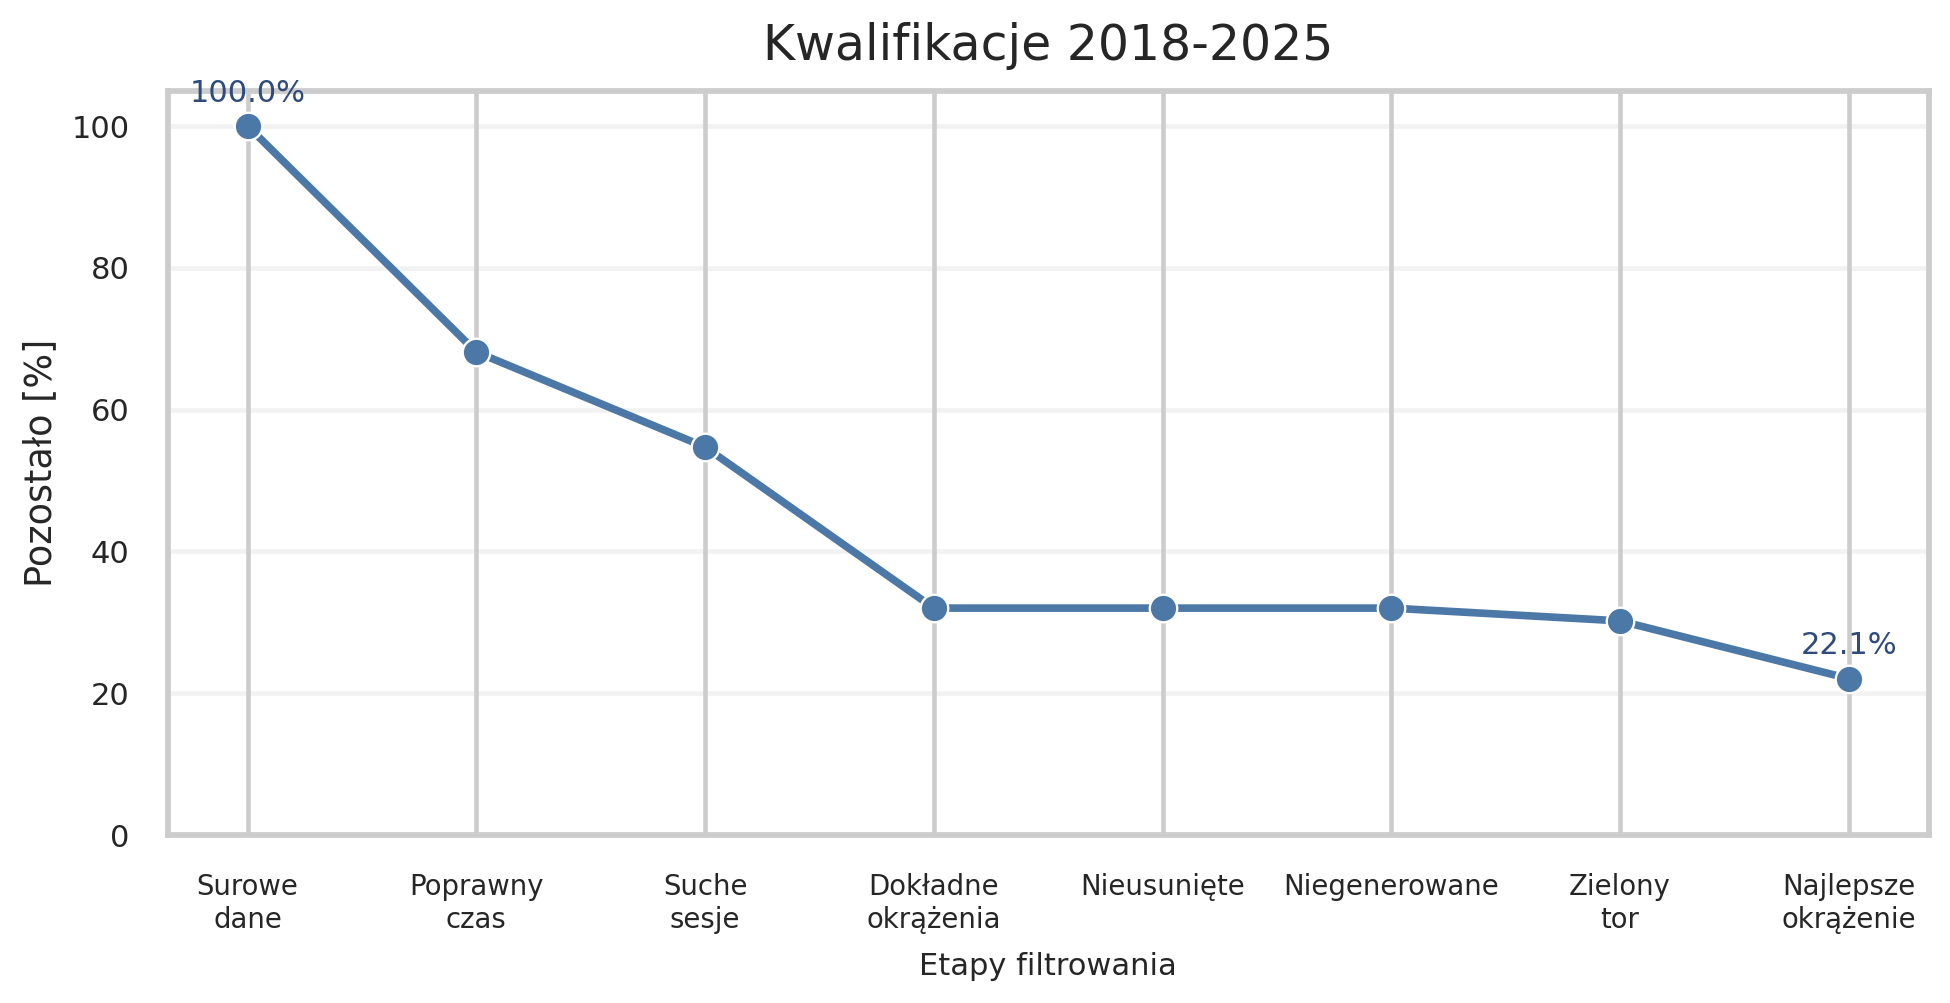
\includegraphics[width=0.92\textwidth]{01b_filter_funnel_qualifying_2018_2025.png}
\caption{Redukcja danych po kolejnych filtrach w setupie kwalifikacyjnym 2018--2025.}
\label{fig:filter-funnel-long-qualifying}
\end{figure}

\begin{figure}[H]
\centering
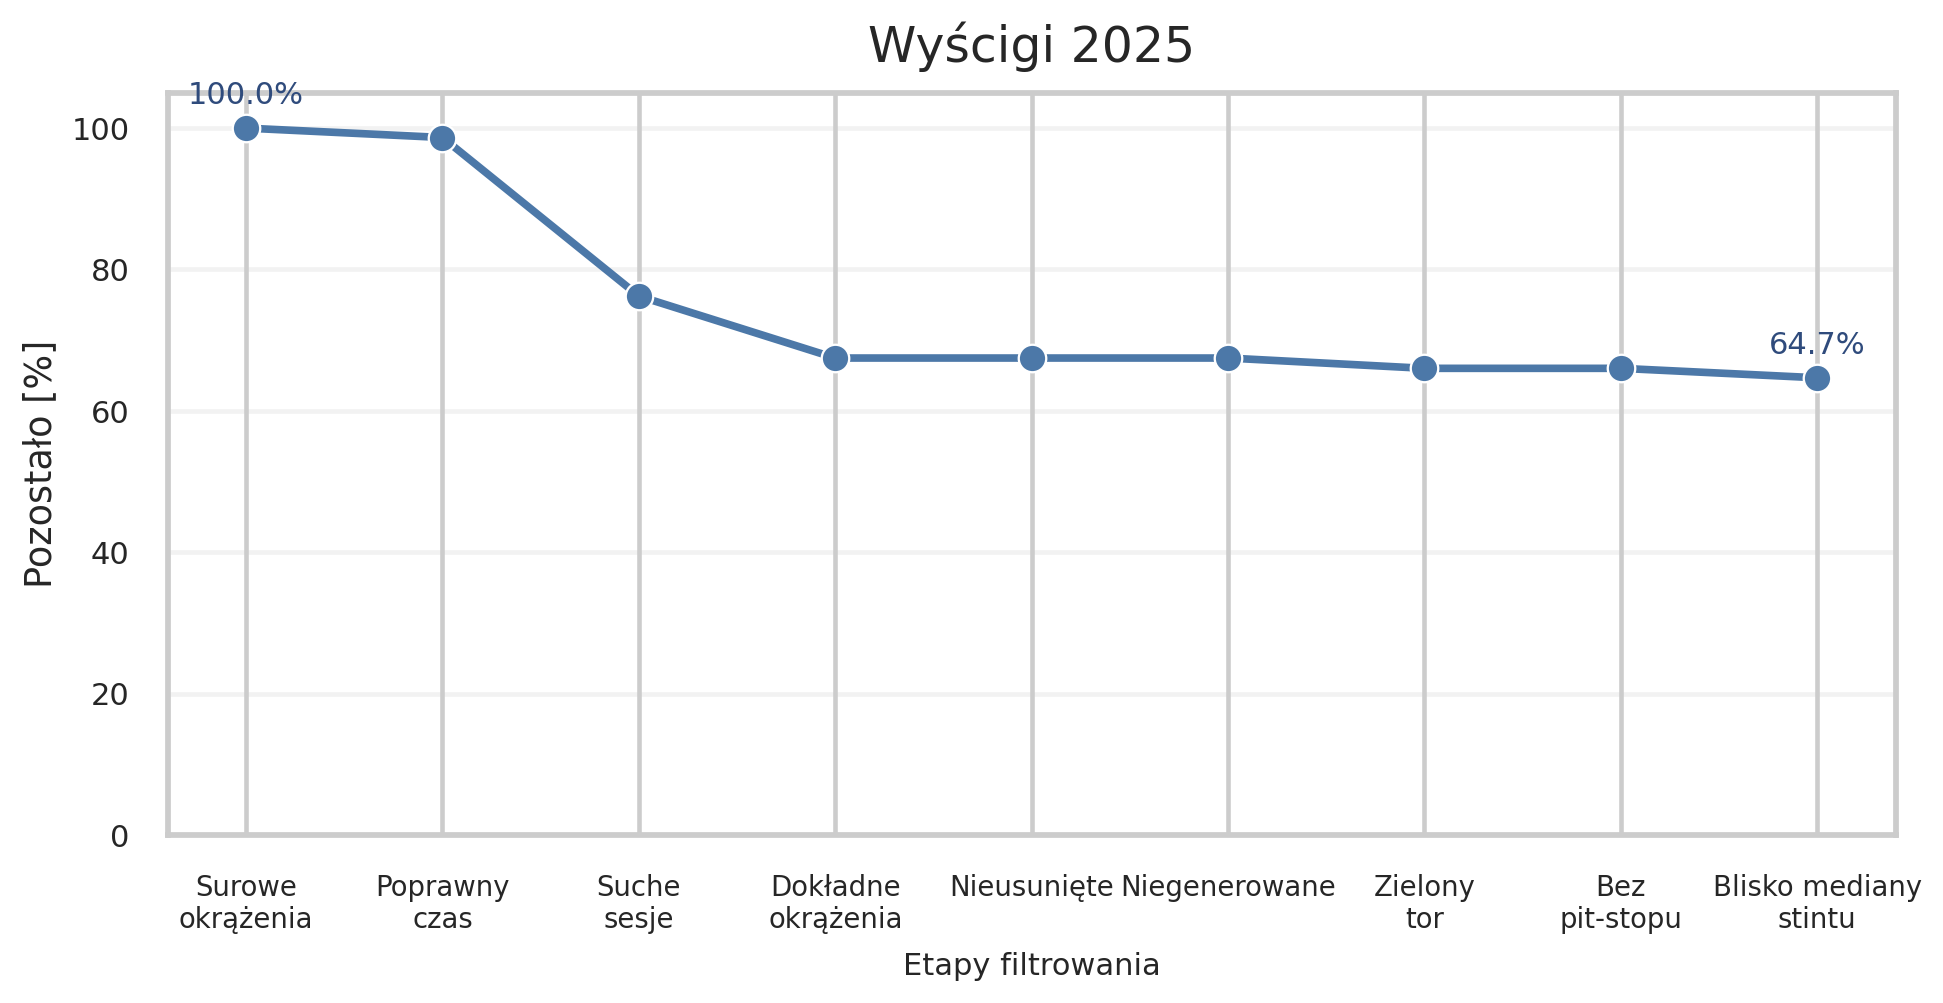
\includegraphics[width=0.92\textwidth]{01c_filter_funnel_race_2025.png}
\caption{Redukcja danych po kolejnych filtrach w setupie wyścigowym 2025.}
\label{fig:filter-funnel-race}
\end{figure}
\FloatBarrier

Największa redukcja w kwalifikacjach wynikała z odrzucenia okrążeń bez poprawnego czasu, ograniczenia danych do suchych sesji oraz wyboru najlepszych reprezentatywnych okrążeń kierowców. Końcowy zbiór kwalifikacyjny jest przez to niewielki i lepiej odpowiada założeniu analizy, czyli porównywaniu okrążeń wykonanych w podobnym trybie jazdy, bez nadmiernego powielania przejazdów z tej samej sesji.

W przypadku wyścigów redukcja wygląda inaczej. Po filtrach jakościowych nadal zostaje duża liczba okrążeń, ponieważ z jednej sesji wyścigowej można wykorzystać wiele czystych okrążeń tego samego kierowcy. Wynika to z innej definicji próbki. W kwalifikacjach wybierane jest głównie jedno reprezentatywne okrążenie, natomiast w wyścigu zachowywane są liczne okrążenia spełniające kryteria czystości.

\section{Wybór kierowców}

Wybór kierowców był istotnym elementem przygotowania eksperymentów. Zamiast analizować przypadkową grupę zawodników, zbudowano zbiór umożliwiający sensowne porównanie różnic stylu jazdy. Punktem startowym był szeroki zbiór kierowców dostępnych w danych, a finalne grupy wybierano na podstawie liczby okrążeń, jakości danych i możliwości stabilnej interpretacji wyników.

Pierwszym kryterium była liczba dostępnych okrążeń. Kierowcy z bardzo krótkim okresem startów, pojedynczymi zastępstwami lub małą liczbą czystych okrążeń wnosili zbyt mało materiału do stabilnego modelowania. W takim przypadku model mógłby uczyć się przypadkowych cech kilku sesji zamiast powtarzalnego profilu jazdy. Dlatego w pierwszych eksperymentach zastosowano próg minimalnej liczby okrążeń, a w późniejszych setupach wybierano kierowców z możliwie dobrym pokryciem sezonów i sesji.

Drugim kryterium była sensowność porównania stylu jazdy. W Formule 1 styl kierowcy tworzy kombinacja kilku zachowań, takich jak sposób wejścia w zakręt, preferencja balansu samochodu, praca gazu, moment rozpoczęcia hamowania, sposób redukcji biegów, utrzymywanie prędkości minimalnej oraz przyspieszanie na wyjściu z zakrętu. Analizy branżowe Formuły 1 \cite{formula1_racing_id, autosport_driving_style} często opisują styl jazdy właśnie przez preferencję nadsterowności lub podsterowności, różnice w kształcie linii przejazdu oraz odmienny sposób zarządzania fazą hamowania i przyspieszania.

Takie opisy potraktowano jako punkt wyjścia do sformułowania problemu badawczego. Jeżeli kierowcy faktycznie różnią się sposobem prowadzenia samochodu, część tych różnic powinna być widoczna w telemetrii. Finalny wybór kierowców opierał się więc na danych oraz jakości późniejszej interpretacji. Eksperyment miał pokazać, czy model potrafi odnaleźć powtarzalne wzorce i czy te wzorce da się później zinterpretować w kategoriach jazdy kierowcy.

Analizę wykonywano także dla większej liczby zawodników, lecz nie w każdym przypadku wyniki były równie czytelne. Część kierowców miała mniej wyraźny profil w publicznej telemetrii, część była silniej przykryta charakterystyką samochodu, a część miała po prostu zbyt mało danych. Dlatego bardziej wartościowe było pokazanie przypadków, w których klasyfikację da się stabilnie omówić, niż utrzymywanie wszystkich kierowców kosztem bardzo nierównych klas i słabszej interpretacji.

W krótkim setupie kwalifikacyjnym finalni kierowcy mieli po 54--55 okrążeń, więc klasy były praktycznie zbalansowane. W kwalifikacjach 2018--2025 wybrana piątka miała od 121 do 145 okrążeń. Ocon miał najmniej danych w tej grupie, jednak jego liczebność nadal pozwalała na modelowanie. W setupie wyścigowym liczba próbek była dużo większa i mieściła się w zakresie 799--911 okrążeń na kierowcę.

Zawężenie listy kierowców potraktowano jako etap projektowania eksperymentu. Najpierw sprawdzono, czy w danych istnieje informacja pozwalająca rozpoznać kierowcę, a następnie skupiono się na grupach, w których tę informację można sensownie interpretować. Część badawcza przechodzi dzięki temu od pytania „czy model rozpoznaje kierowcę?” do ważniejszego pytania „jakie cechy telemetrii pozwalają go rozpoznać?”.

\section{Typy zmiennych i braki danych}

W danych występują identyfikatory okrążeń, kolumny kontekstowe, zmienne kategoryczne oraz numeryczne cechy modelowe. Większość cech wykorzystywanych przez modele ma charakter numeryczny, ponieważ powstaje przez agregację sygnałów telemetrycznych. Do wejścia modeli trafiały wyłącznie informacje opisujące przebieg okrążenia i wybrany kontekst eksperymentu. Identyfikatory takie jak \texttt{lap\_key}, etykieta \texttt{Driver} oraz kolumny jednoznacznie wskazujące konkretną próbkę zostały pominięte, ponieważ prowadziłyby do przecieku informacji albo sztucznego ułatwienia zadania.

Zmienne kategoryczne były traktowane ostrożnie. Część z nich, np. nazwa kierowcy, pełniła rolę etykiety modelu. Inne, takie jak \texttt{Team} lub kontekst sesji, mogły wprowadzać informację o samochodzie zamiast o samym kierowcy, dlatego były używane tylko w wybranych eksperymentach kontrolnych. Jeżeli zmienne kategoryczne były używane w modelach tabularnych, wymagały kodowania, natomiast w głównych wariantach interpretacyjnych nacisk położono na cechy numeryczne pochodzące z telemetrii.

Braki danych w numerycznych cechach modelowych były bardzo małe. W krótkim setupie kwalifikacyjnym pojedyncze braki dotyczyły głównie informacji o oponach, np. \texttt{TyreLife}. Zasadnicze sygnały telemetryczne i cechy zagregowane były kompletne. W długim setupie kwalifikacyjnym i w setupie wyścigowym najważniejsze cechy modelowe nie miały braków, więc nie stosowano złożonej strategii imputacji.

\section{Reprezentacja okrążenia}

Każde okrążenie opisano dwiema reprezentacjami:

\begin{itemize}
    \item jako wektor ręcznie zdefiniowanych cech, np. średnia prędkość, udział pełnego gazu, liczba aktywacji hamulca, liczba zmian biegów;
    \item jako sekwencja telemetryczna z sygnałami \texttt{Speed}, \texttt{Throttle}, \texttt{Brake}, \texttt{RPM}, \texttt{nGear}.
\end{itemize}

\begin{figure}[H]
\centering
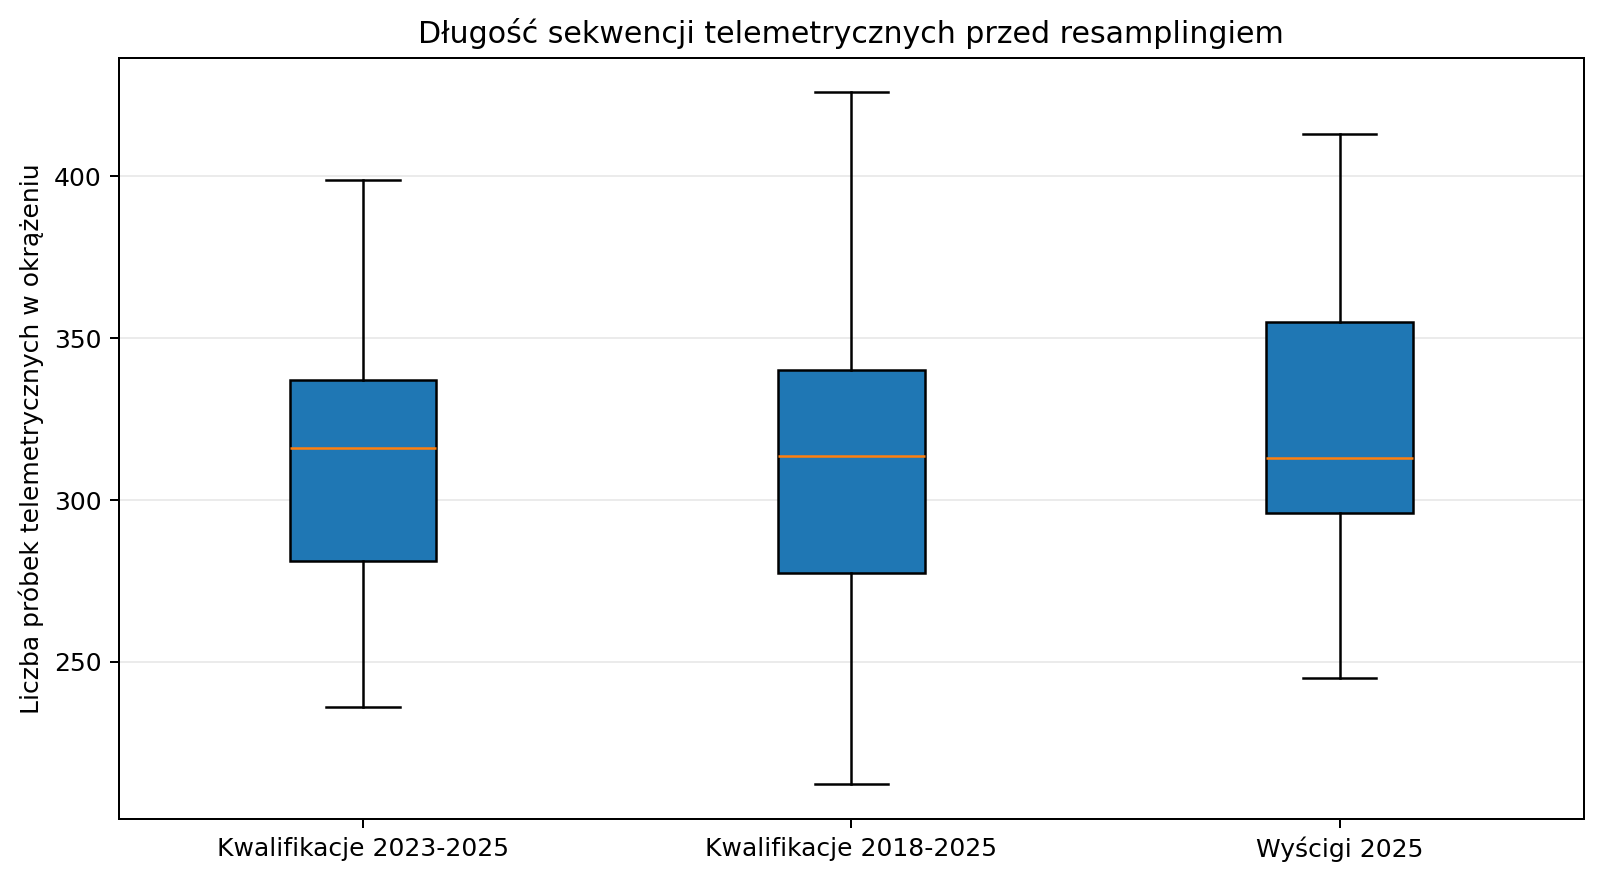
\includegraphics[width=0.90\textwidth]{27_eda_sequence_lengths.png}
\caption{Długość sekwencji telemetrycznych przed resamplingiem.}
\label{fig:eda-sequence-lengths}
\end{figure}

Sekwencje telemetryczne miały zmienną długość, dlatego przed treningiem modeli sekwencyjnych były resamplowane do stałej liczby próbek. Zmienność długości wynika z czasu okrążenia i sposobu próbkowania danych. Rozkład długości nie wskazywał jednak na problem uniemożliwiający uczenie modeli sekwencyjnych.

\section{Korelacje cech}

Przed modelowaniem warto sprawdzić, czy wybrane cechy opisują niezależne informacje, czy raczej różne ujęcia tego samego zjawiska. W danych telemetrycznych silna korelacja części cech jest oczekiwana, ponieważ prędkość, biegi, obroty silnika i praca przepustnicy są ze sobą fizycznie powiązane.

\begin{figure}[H]
\centering
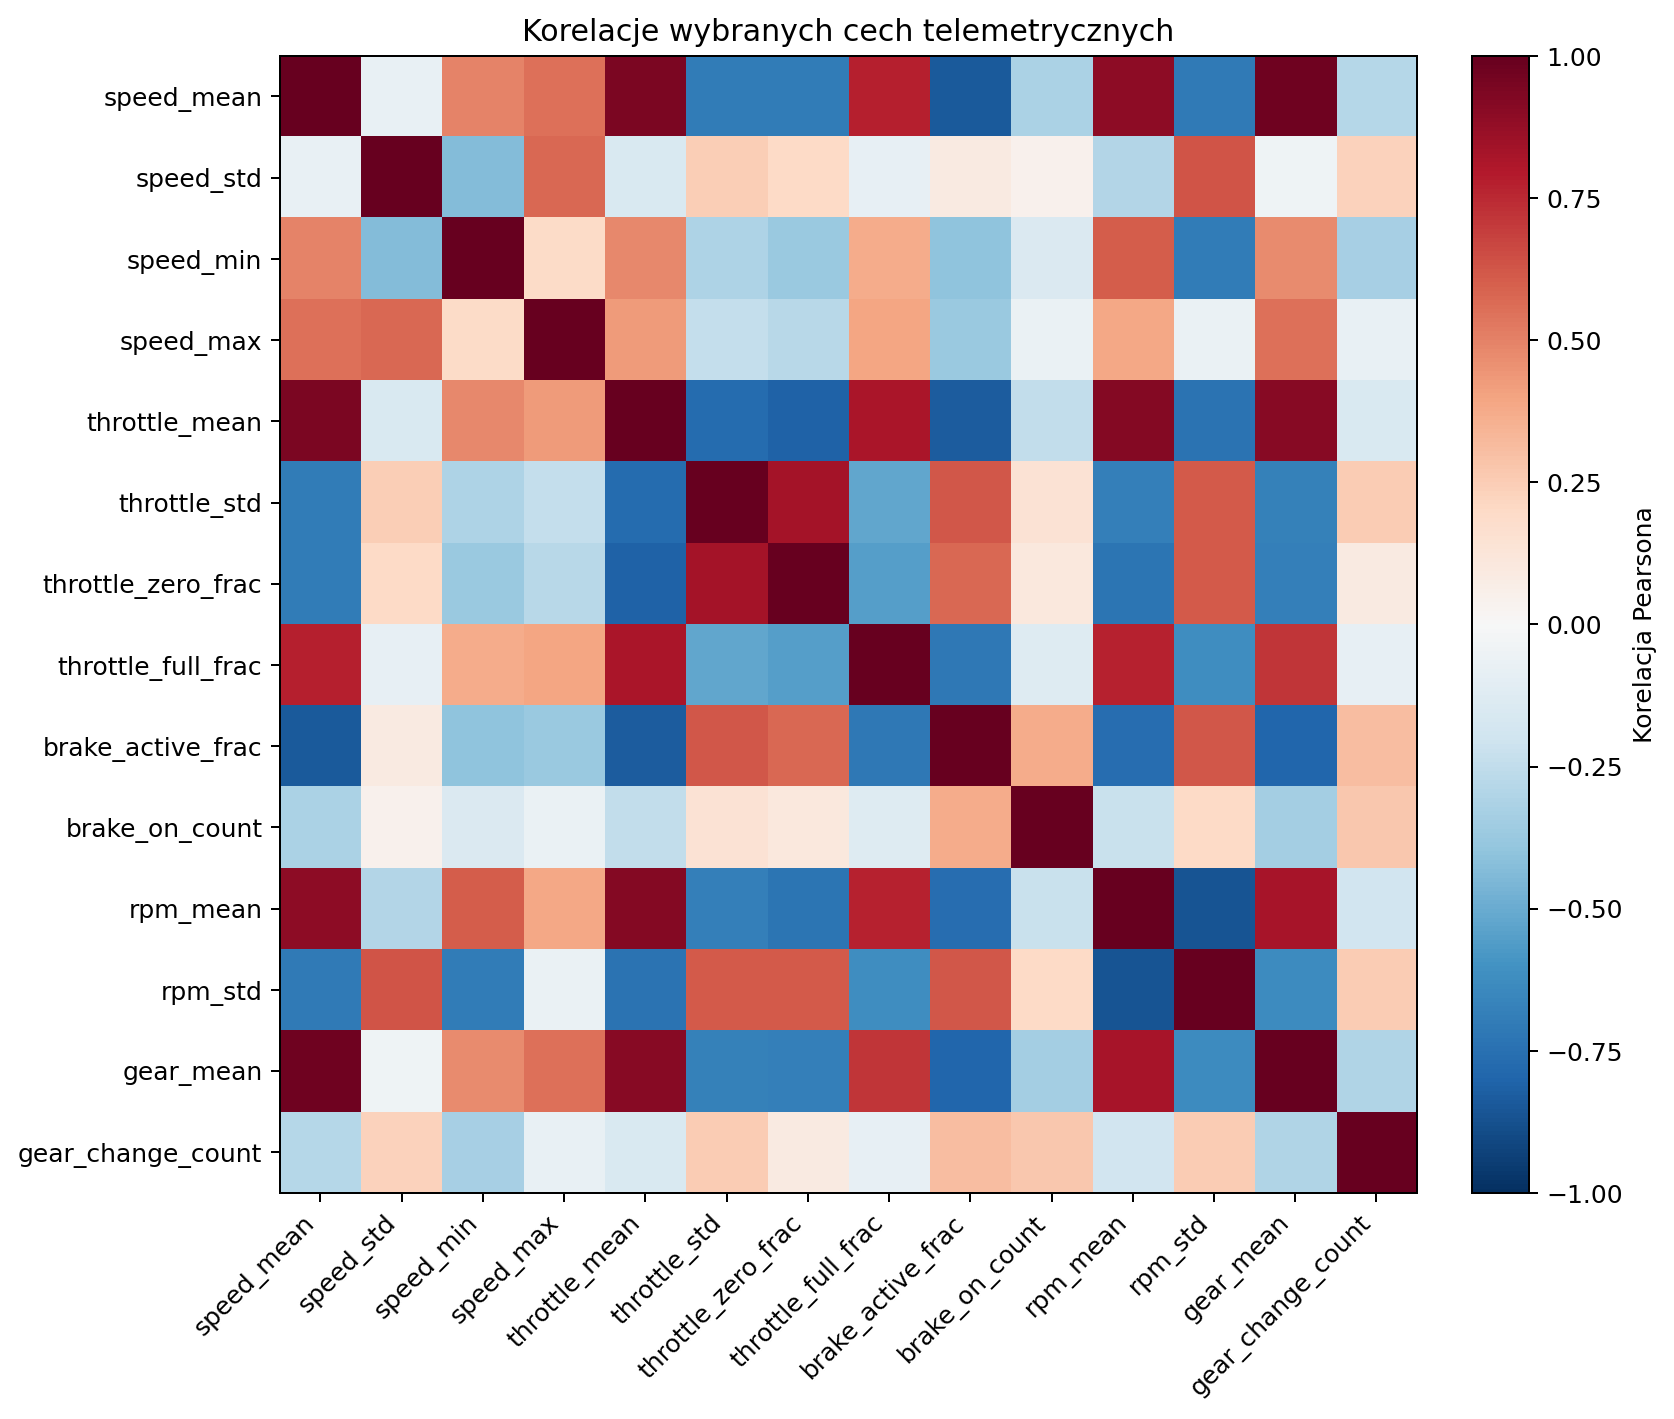
\includegraphics[width=0.90\textwidth]{29_eda_feature_correlation_heatmap.png}
\caption{Korelacje wybranych cech telemetrycznych.}
\label{fig:eda-correlation}
\end{figure}

Na macierzy korelacji widać między innymi powiązania między statystykami prędkości, takimi jak średnia prędkość, kwantyle prędkości i zakres prędkości. Taka zależność jest oczekiwana, ponieważ wszystkie te cechy opisują ogólny profil tempa okrążenia oraz charakter toru. Podobnie korelują ze sobą cechy przepustnicy. Udział pełnego gazu, udział jazdy bez gazu i zmienność sygnału gazu opisują różne strony tego samego zachowania kierowcy.

Widać również związek między cechami obrotów silnika i biegów, ponieważ przełożenie, prędkość i zakres obrotów są mechanicznie powiązane. Z tego powodu interpretacja modelu powinna obejmować całe rodziny cech, takie jak prędkość, gaz, hamowanie, biegi, obroty oraz dynamika sygnałów, zamiast pojedynczej zmiennej analizowanej w izolacji.

\section{Wnioski z eksploracji danych dla modelowania}

Eksploracyjna analiza danych pomogła opisać zbiory oraz podjąć decyzje projektowe. Trzy setupy mają różny charakter i wymagają osobnej interpretacji. Krótkie kwalifikacje 2023--2025 są najbardziej kontrolowane, ponieważ obejmują najnowsze sezony i bardzo czyste okrążenia. Kwalifikacje 2018--2025 są trudniejsze, bo obejmują więcej sezonów, zmian regulaminowych i zmian samochodów. Setup wyścigowy 2025 jest największy, a jednocześnie zawiera bardziej zróżnicowany kontekst związany ze stintem, degradacją opon i przebiegiem wyścigu.

Różnica między setupami wpływa na interpretację wyników. Wynik ograniczony do krótkich kwalifikacji mógłby sugerować zależność od bardzo specyficznych warunków. Skuteczność utrzymująca się również w długim horyzoncie i w czystych okrążeniach wyścigowych wzmacnia argument o obecności mierzalnych wzorców kierowcy. Dlatego wyniki są prezentowane jako porównanie trzech wariantów tego samego problemu, zamiast jednego zbiorczego eksperymentu.

Analiza braków danych pokazała, że zasadnicze sygnały telemetryczne są wystarczająco kompletne do modelowania. Prosta imputacja była wystarczająca i pozwalała uniknąć dodatkowych założeń wprowadzanych przez bardziej rozbudowane metody uzupełniania braków. Zmienna długość sekwencji mieściła się w stabilnym zakresie, a przed modelami sekwencyjnymi zastosowano resampling do wspólnej długości.

Macierz korelacji pokazała natomiast, że część cech opisuje podobne zjawiska fizyczne. W danych telemetrycznych jest to spodziewane i wpływa na interpretację modeli. Dlatego w dalszej analizie większe znaczenie ma interpretowanie grup cech, na przykład tych związanych z prędkością, gazem, hamowaniem, biegami i obrotami, niż pojedynczej zmiennej oderwanej od pozostałych. Ten wniosek jest później szczególnie istotny przy omawianiu najważniejszych cech regresji logistycznej.

EDA uzasadniła też potrzebę analizy biasu zespołowego. Część cech telemetrycznych może wynikać ze stylu kierowcy, charakterystyki samochodu, zespołu, toru i sezonu. Sama wysoka skuteczność rozpoznawania kierowcy nie wystarczała do interpretacji wyników. Dlatego sprawdzono, czy podobne dane pozwalają rozpoznawać zespół oraz czy model nadal rozróżnia kierowców w sytuacjach, w których jeżdżą oni tym samym samochodem.

\section{Ograniczenia danych}

Najważniejsze ograniczenia danych:

\begin{itemize}
    \item publiczna telemetria nie zawiera pełnego kąta skrętu kierownicy;
    \item kanał \texttt{Brake} jest w praktyce sygnałem binarnym;
    \item dane pozycyjne i dane samochodu wymagają dokładniejszego wyrównania czasowego przed analizą zakręt po zakręcie;
    \item styl kierowcy jest częściowo spleciony z charakterystyką samochodu i zespołu.
\end{itemize}

Te ograniczenia wpływają na zakres wniosków. Wyniki pozwalają mówić o rozpoznawaniu kierowcy i o cechach telemetrycznych związanych z tym rozpoznawaniem, z zachowaniem ostrożności przy pełnym opisie techniki jazdy. Szczególnie uważnie trzeba interpretować cechy zależne od samochodu, takie jak prędkości, biegi czy obroty silnika. Dlatego dalsze rozdziały obejmują klasyfikację kierowcy, analizę wpływu zespołu oraz testy porównujące kierowców w obrębie tego samego samochodu.

\chapter{Metodyka eksperymentów}

\section{Proces, modele, walidacja i metryki}

Metodyka pracy została podzielona na kilka etapów odpowiadających kolejnym decyzjom badawczym. Obejmowała przygotowanie danych, wybór reprezentacji okrążenia, porównanie modeli i interpretację wyników. Najpierw zbudowano zbiory okrążeń spełniających przyjęte kryteria jakości, następnie przygotowano dwie reprezentacje danych, a na końcu porównano modele klasyfikacyjne w trzech setupach eksperymentalnych.

Pełny proces obejmował:

\begin{enumerate}
    \item audyt dostępności sesji i danych;
    \item filtrowanie okrążeń;
    \item wybór reprezentatywnych okrążeń;
    \item ekstrakcję telemetrii;
    \item budowę cech tabularnych;
    \item resampling sekwencji;
    \item trenowanie i walidację modeli;
    \item interpretację wyników i analizę wpływu zespołu.
\end{enumerate}

Pierwsza grupa eksperymentów korzystała z ręcznie zdefiniowanych cech opisujących całe okrążenie, takich jak średnia prędkość, udział pełnego gazu, liczba aktywacji hamulca czy liczba zmian biegów. Na tej reprezentacji porównano regresję logistyczną, Random Forest oraz modele boostingowe. Regresja logistyczna została potraktowana jako główny model interpretowalny, ponieważ pozwala analizować współczynniki cech i wskazywać, które elementy telemetrii najbardziej wpływają na decyzję modelu. Modele drzewiaste i boostingowe pełniły rolę punktu porównawczego dla danych tabularnych.

Druga grupa eksperymentów analizowała całe przebiegi telemetryczne jako szeregi czasowe. Taka reprezentacja pozwala zachować kolejność zdarzeń w trakcie przejazdu oraz lokalne wzorce, które mogą zanikać po agregacji do pojedynczych statystyk. W tej części porównano architektury \texttt{1D CNN}, \texttt{GRU}, \texttt{LSTM} oraz model hybrydowy \texttt{CNN + cechy tabularne}.

Główną metodą walidacji był \texttt{StratifiedGroupKFold}, gdzie grupą była sesja. Taki podział ogranicza przeciek informacji pomiędzy zbiorem treningowym i testowym, ponieważ wszystkie okrążenia z tej samej sesji pozostają po jednej stronie podziału. Najważniejszą metryką była wartość macro F1, ponieważ klasy mogą mieć różną liczebność, a każdy kierowca powinien mieć podobny wpływ na wynik końcowy. Dodatkowo raportowano accuracy, balanced accuracy, macierze pomyłek oraz różnice między wynikiem treningowym i testowym.

\section{Protokół walidacji i preprocessingu}

W każdym głównym eksperymencie zastosowano pięciofoldową walidację krzyżową. W takim schemacie każda próbka trafia do części testowej dokładnie raz, a raportowany wynik powstaje z predykcji out-of-fold albo ze średniej wyników na foldach testowych. Podział odpowiada w przybliżeniu proporcji 80/20 między treningiem i testem w każdym foldzie. Dokładne proporcje zależą jednak od liczby okrążeń przypadających na sesje, ponieważ walidacja była grupowana.

Grupą w walidacji była sesja, identyfikowana przez \texttt{session\_key}, a w starszych eksportach przez parę sezon--runda. Oznacza to, że wszystkie okrążenia z jednej sesji trafiały albo do treningu, albo do testu. Ma to duże znaczenie, ponieważ okrążenia z tej samej sesji dzielą tor, warunki pogodowe, kontekst weekendu oraz charakterystykę samochodu w danym wydarzeniu. Bez grupowania model mógłby uzyskać zawyżony wynik, ucząc się specyfiki sesji zamiast wzorców kierowcy.

\begin{table}[H]
\centering
\small
\begin{tabular}{lccccc}
\toprule
Setup & Liczba foldów & Liczba sesji & Średni trening & Walidacja wewn. & Średni test \\
\midrule
Kwalifikacje 2023--2025 & 5 & 55 & 218.4 & 45.0 & 54.6 \\
Kwalifikacje 2018--2025 & 5 & 146 & 558.4 & 112.0 & 139.6 \\
Wyścigi 2025 & 5 & 18 & 3467.2 & 663.4 & 866.8 \\
\bottomrule
\end{tabular}
\caption{Liczba foldów, liczba sesji oraz średnie rozmiary części treningowej, walidacyjnej i testowej w schemacie walidacji. Kolumna walidacji wewnętrznej dotyczy modeli sekwencyjnych i hybrydowych.}
\label{tab:outer-fold-sizes}
\end{table}

Liczba okrążeń nie jest tożsama z liczbą niezależnych obserwacji. Ponieważ walidacja jest grupowana po sesjach, a okrążenia z jednej sesji są silnie skorelowane, efektywna liczba niezależnych jednostek jest bliższa liczbie sesji niż liczbie okrążeń. Dotyczy to zwłaszcza setupu wyścigowego, w którym 4334 okrążenia pochodzą z 18 sesji. Duża liczba próbek zwiększa ilość danych treningowych, ale nie usuwa całkowicie zależności wewnątrz pojedynczego weekendu wyścigowego.

Preprocessing modeli tabularnych był wykonywany wewnątrz obiektu \texttt{Pipeline} biblioteki \texttt{scikit-learn}. Dla cech numerycznych stosowano imputację medianą oraz standaryzację \texttt{StandardScaler}; dla cech kategorycznych, jeżeli dana konfiguracja je zawierała, stosowano imputację najczęstszą wartością oraz kodowanie \texttt{OneHotEncoder}. Parametry imputacji, skalowania i kodowania były dopasowywane wyłącznie na części treningowej danego folda, a następnie używane do transformacji części testowej. Dzięki temu test fold nie wpływał na preprocessing.

W modelach sekwencyjnych każdy outer fold miał dodatkowy wewnętrzny podział walidacyjny. Najpierw wydzielano zewnętrzny fold testowy, niewykorzystywany podczas treningu. Następnie w obrębie części treningowej wybierano wewnętrzny fold walidacyjny służący do \emph{early stoppingu}. Standaryzację sekwencji oraz cech tabularnych w modelu hybrydowym wyznaczano na części treningowej bez danych walidacyjnych i testowych, a następnie stosowano do walidacji oraz testu. Dzięki temu zewnętrzny fold testowy pozostawał odseparowany od decyzji podejmowanych podczas treningu.

Dobór hiperparametrów rozdzielono od oceny końcowej. W osobnej fazie eksploracyjnej porównano rodziny modeli oraz konfiguracje cech, a następnie wybrane konfiguracje zamrożono. Tak ustalone konfiguracje oceniano w pięciofoldowej walidacji krzyżowej grupowanej po sesjach, bez zagnieżdżonego przeszukiwania hiperparametrów wewnątrz poszczególnych foldów. Oznacza to, że raportowane wyniki odpowiadają stałym konfiguracjom, a nie pipeline'owi strojonemu osobno dla każdego podziału. Parametry preprocessingu dopasowywano wyłącznie na części treningowej danego folda, a moment zatrzymania treningu modeli sekwencyjnych wynikał z wewnętrznego zbioru walidacyjnego. Konsekwencją takiego protokołu jest to, że wybór architektur i cech był poinformowany całością danych w fazie eksploracyjnej, co może prowadzić do umiarkowanie optymistycznego oszacowania wyników; pełne, zagnieżdżone strojenie hiperparametrów (nested cross-validation) pozostaje kierunkiem dalszej pracy.

\section{Parametry modeli tabularnych}

Modele tabularne trenowano w tych samych zewnętrznych foldach co modele sekwencyjne. W finalnych eksperymentach identyfikacji kierowcy głównym modelem była regresja logistyczna z regularyzacją L1. Modele drzewiaste i boostingowe pełniły funkcję punktu porównawczego oraz kontroli, czy bardziej elastyczne klasyfikatory tabularne nie dają lepszego wyniku.

\begin{table}[H]
\centering
\footnotesize
\setlength{\tabcolsep}{5pt}
\renewcommand{\arraystretch}{1.2}
\begin{tabularx}{\textwidth}{%
  >{\raggedright\arraybackslash}p{3.5cm}%
  >{\raggedright\arraybackslash}p{2.5cm}%
  >{\raggedright\arraybackslash}p{2.6cm}%
  >{\raggedright\arraybackslash}X}
\toprule
Model & Regularyzacja / struktura & Iteracje lub drzewa & Pozostałe parametry \\
\midrule
Regresja logistyczna, krótki setup & L1, \(C=2.0\) & maks. 7000 iteracji & solver \texttt{saga} \\
Regresja logistyczna, długi setup i wyścigi & L1, \(C=2.0\) & maks. 5000 iteracji & solver \texttt{saga} \\
Random Forest & brak limitu głębokości & 400 drzew & \texttt{min\_samples\_leaf=1} \\
Hist\-Gradient\-Boosting & głębokość maks. 6 & 300 iteracji & \texttt{learning\_rate=0.05} \\
XGBoost & głębokość maks. 6 & 300 drzew & \texttt{learning\_rate=0.05},\newline \texttt{subsample=0.9},\newline \texttt{colsample\_bytree=0.9} \\
\bottomrule
\end{tabularx}
\caption{Najważniejsze parametry modeli tabularnych użytych w głównych porównaniach.}
\label{tab:tabular-model-params}
\end{table}

\section{Specyfikacja modeli sekwencyjnych}

Wejściem modeli sekwencyjnych była sekwencja o długości 300 punktów. Każdy punkt zawierał pięć kanałów: \texttt{Speed}, \texttt{Throttle}, \texttt{Brake}, \texttt{RPM} oraz \texttt{nGear}. Zmienną długość oryginalnych okrążeń wyrównano przez liniowy resampling do wspólnej długości. Tabela~\ref{tab:sequence-architecture-spec} przedstawia architektury wykorzystane w eksperymentach.

\begin{table}[H]
\centering
\footnotesize
\setlength{\tabcolsep}{5pt}
\renewcommand{\arraystretch}{1.25}
\begin{tabularx}{\textwidth}{%
  >{\raggedright\arraybackslash}p{1.9cm}%
  >{\raggedright\arraybackslash}X%
  >{\raggedright\arraybackslash}p{3.7cm}%
  >{\raggedright\arraybackslash}p{2.7cm}}
\toprule
Model & Główna część modelu & Agregacja / połączenie & Klasyfikator \\
\midrule
\texttt{CNN} & cztery warstwy \texttt{Conv1D}: 32 filtry z \(k=7\), następnie 64 filtry z \(k=5\) & \texttt{MaxPool(2)}, \texttt{GlobalAveragePooling}, dropout 0.2--0.3 & \texttt{Dense(64)} i warstwa \texttt{softmax} \\
\texttt{CNN + tabular} & gałąź sekwencyjna \texttt{CNN}; gałąź tabularna \texttt{Dense(32)} & połączenie przez \texttt{Concatenate}, dropout 0.2--0.3 & \texttt{Dense(64)} i warstwa \texttt{softmax} \\
\texttt{GRU} & dwie warstwy \texttt{GRU}: 64 i 32 jednostki & dropout 0.2--0.3 & \texttt{Dense(64)} i warstwa \texttt{softmax} \\
\texttt{LSTM} & dwie warstwy \texttt{LSTM}: 64 i 32 jednostki & dropout 0.2--0.3 & \texttt{Dense(64)} i warstwa \texttt{softmax} \\
\bottomrule
\end{tabularx}
\caption{Specyfikacja architektur sekwencyjnych i hybrydowych.}
\label{tab:sequence-architecture-spec}
\end{table}

Funkcją straty była \texttt{sparse\_categorical\_crossentropy}, ponieważ zadanie ma charakter wieloklasowy, a etykiety kierowców były kodowane jako numery klas. Jako optymalizator wybrano \texttt{Adam} z learning rate równym 0.001, czyli stabilny punkt startowy dla sieci tego typu. W długim setupie kwalifikacyjnym i w setupie wyścigowym użyto batch size równego 32. W pierwotnym eksperymencie krótkohoryzontowym batch size wynosił 16, ponieważ ten etap był wykonany wcześniej jako osobny notebook eksploracyjny. W każdym przypadku stosowano early stopping na podstawie \texttt{val\_loss} z przywróceniem najlepszych wag. Nie stosowano harmonogramu zmiany kroku uczenia (\emph{learning rate scheduler}); jedynym mechanizmem regulującym długość treningu był early stopping. Wagi inicjalizowano domyślnymi metodami biblioteki \texttt{Keras}. Pełna specyfikacja architektur znajduje się w tabeli~\ref{tab:sequence-architecture-spec}, a parametry treningu w tabeli~\ref{tab:sequence-training-params}.

\begin{table}[H]
\centering
\small
\begin{tabular}{lccc}
\toprule
Setup & Maks. liczba epok & Patience & Batch size \\
\midrule
Kwalifikacje 2023--2025 & 150 & 20 & 16 \\
Kwalifikacje 2018--2025 & 80 & 10 & 32 \\
Wyścigi 2025 & 60 & 8 & 32 \\
\bottomrule
\end{tabular}
\caption{Parametry treningu modeli sekwencyjnych i hybrydowych.}
\label{tab:sequence-training-params}
\end{table}

\section{Raportowanie niepewności wyników}

Wyniki modeli raportowano jako macro F1 out-of-fold oraz jako średnią i odchylenie standardowe wyników na foldach testowych. Dodatkowo dla głównych porównań przygotowano bootstrapowy 95\% przedział ufności średniej wartości macro F1 po foldach oraz porównania parowane między modelami w obrębie tych samych foldów. Ze względu na pięć foldów testy parowane pełnią funkcję pomocniczej informacji o stabilności różnicy. Wnioski oparto przede wszystkim na połączeniu wartości średniej, rozrzutu między foldami, macierzy pomyłek oraz zgodności wyników między trzema setupami.

Dla zapewnienia powtarzalności cały proces, od filtrowania okrążeń przez ekstrakcję telemetrii po trening i walidację, wykonano w jednym, opisanym powyżej potoku przetwarzania. Dane pobierano biblioteką FastF1 w wersji 3.8.1, modele tabularne budowano w oparciu o potoki \texttt{scikit-learn}, a modele sekwencyjne trenowano w bibliotece \texttt{Keras}. Podział na foldy wynikał jednoznacznie z grupowania po sesjach, a parametry preprocessingu dopasowywano wyłącznie na części treningowej każdego folda, dzięki czemu schemat walidacji jest deterministyczny i odtwarzalny na tych samych danych.

\chapter{Badanie 1: Identyfikacja kierowcy na podstawie telemetrii}

Pierwsze badanie dotyczyło rozpoznawania kierowcy na podstawie danych telemetrycznych. Porównano modele oparte na ręcznie zdefiniowanych cechach z modelami sekwencyjnymi i hybrydowymi.

\section{Punkt odniesienia: regresja logistyczna}

Pierwszym właściwym modelem była regresja logistyczna trenowana na ręcznie zdefiniowanych cechach. Ten model pełnił rolę punktu odniesienia, ponieważ jest prostszy do interpretacji niż sieci neuronowe i pozwala analizować współczynniki przypisane poszczególnym cechom.

Na początku sprawdzono szerszy zbiór 14 kierowców, a następnie przeprowadzono wybór bardziej rozróżnialnej piątki kierowców. W krótkim setupie kwalifikacyjnym pozwoliło to przejść od szerokiego baseline'u do finalnego modelu dla kierowców \texttt{ALB}, \texttt{SAI}, \texttt{VER}, \texttt{OCO} i \texttt{LEC}. W tym wariancie regresja logistyczna osiągnęła 0.8617 macro F1 w predykcjach out-of-fold, a średni wynik na foldach testowych wyniósł \(0.8608 \pm 0.0193\).

\begin{figure}[H]
\centering
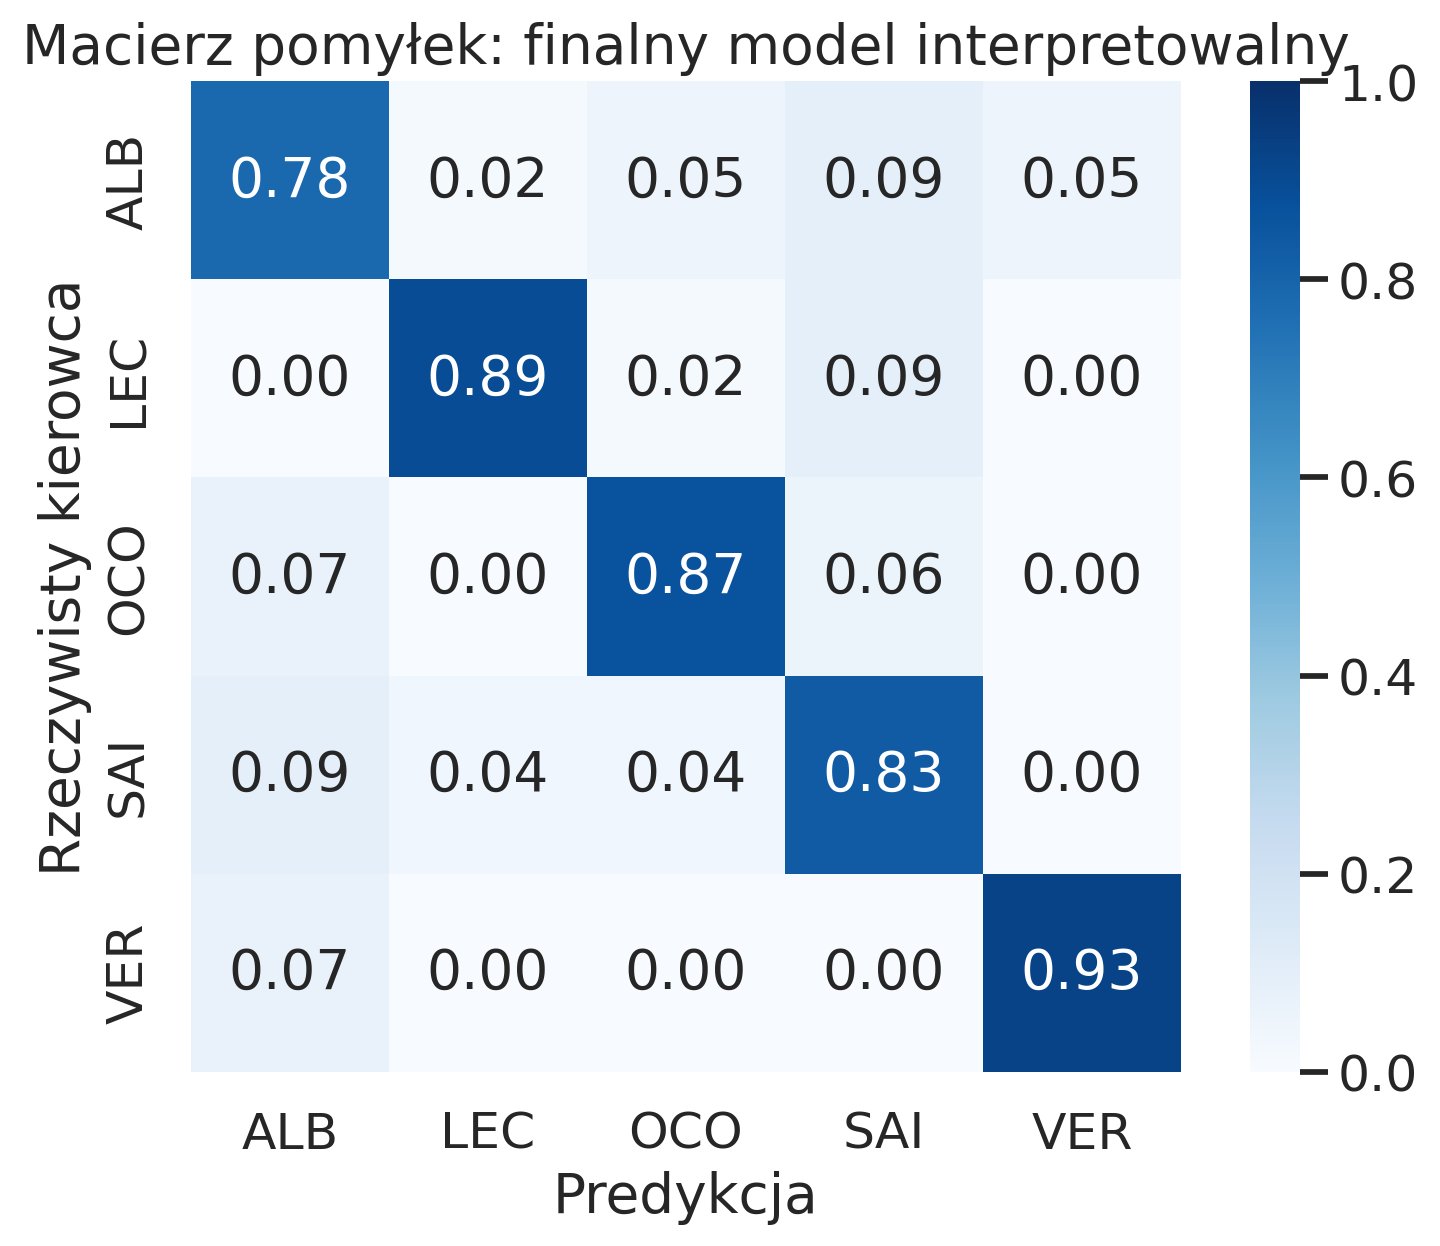
\includegraphics[width=0.52\textwidth]{05_final_model_confusion_matrix.png}
\caption{Macierz pomyłek finalnego modelu regresji logistycznej w krótkim setupie kwalifikacyjnym.}
\label{fig:final-confusion}
\end{figure}

Ten wynik jest zgodny z ogólnym kierunkiem badań nad identyfikacją kierowcy z danych pojazdu, w których zakłada się, że indywidualne zachowania kierowcy są widoczne w sygnałach takich jak prędkość, hamowanie czy przyspieszanie \cite{hallac2016,wang2017}. W danych Formuły 1 problem jest trudniejszy, ponieważ kierowcy jeżdżą dużo bardziej podobnie pod względem celu i wszyscy starają się uzyskać możliwie najlepszy czas. Stabilny wynik w takim środowisku sugeruje, że nawet na bardzo wysokim poziomie sportowym pozostaje mierzalna indywidualna różnica w przebiegu okrążenia.

Istotnym elementem tej części było sprawdzenie wpływu prostego tempa okrążenia. W kolejnych wariantach usuwano bezpośrednie cechy czasowe, takie jak \texttt{LapTimeSeconds} oraz czasy sektorów. W setupie wyścigowym najlepszy wariant regresji logistycznej bez cech czasowych i bez części kontekstu wyścigowego uzyskał 0.8177 macro F1, czyli wynik praktycznie taki sam jak warianty zawierające więcej informacji kontekstowej. Taki rezultat sugeruje, że model korzystał także z cech opisujących sposób przejazdu, wykraczających poza samą informację o tempie okrążenia.

Regresja logistyczna okazała się najstabilniejszym modelem tabularnym. W długim setupie kwalifikacyjnym oraz w setupie wyścigowym modele drzewiaste i boostingowe osiągały często wynik treningowy bliski 1.0 macro F1, przy wyraźnie niższym wyniku testowym. Taki train-test gap wskazuje na przeuczenie i uzasadnia pozostawienie regresji logistycznej jako głównego modelu tabularnego. Interpretacja wyników opierała się przede wszystkim na zachowaniu modelu na foldach testowych.

\section{Model sekwencyjny CNN}

Drugim krokiem było przejście od cech zagregowanych do pełnej sekwencji telemetrycznej. W tym podejściu okrążenie było reprezentowane jako przebieg sygnałów \texttt{Speed}, \texttt{Throttle}, \texttt{Brake}, \texttt{RPM} i \texttt{nGear}. Sekwencje były resamplowane do stałej długości, aby mogły być wejściem sieci neuronowej.

Model \texttt{1D CNN} okazał się bardzo mocnym wariantem. W krótkim setupie kwalifikacyjnym poprawił wynik względem regresji logistycznej z 0.8617 do 0.8952 macro F1 w predykcjach out-of-fold, przy średniej foldowej \(0.8941 \pm 0.0479\). W długim setupie kwalifikacyjnym 2018--2025 był najlepszym modelem spośród porównanych architektur sekwencyjnych i osiągnął 0.9012 macro F1, przy średniej foldowej \(0.9011 \pm 0.0264\).

\begin{figure}[H]
\centering
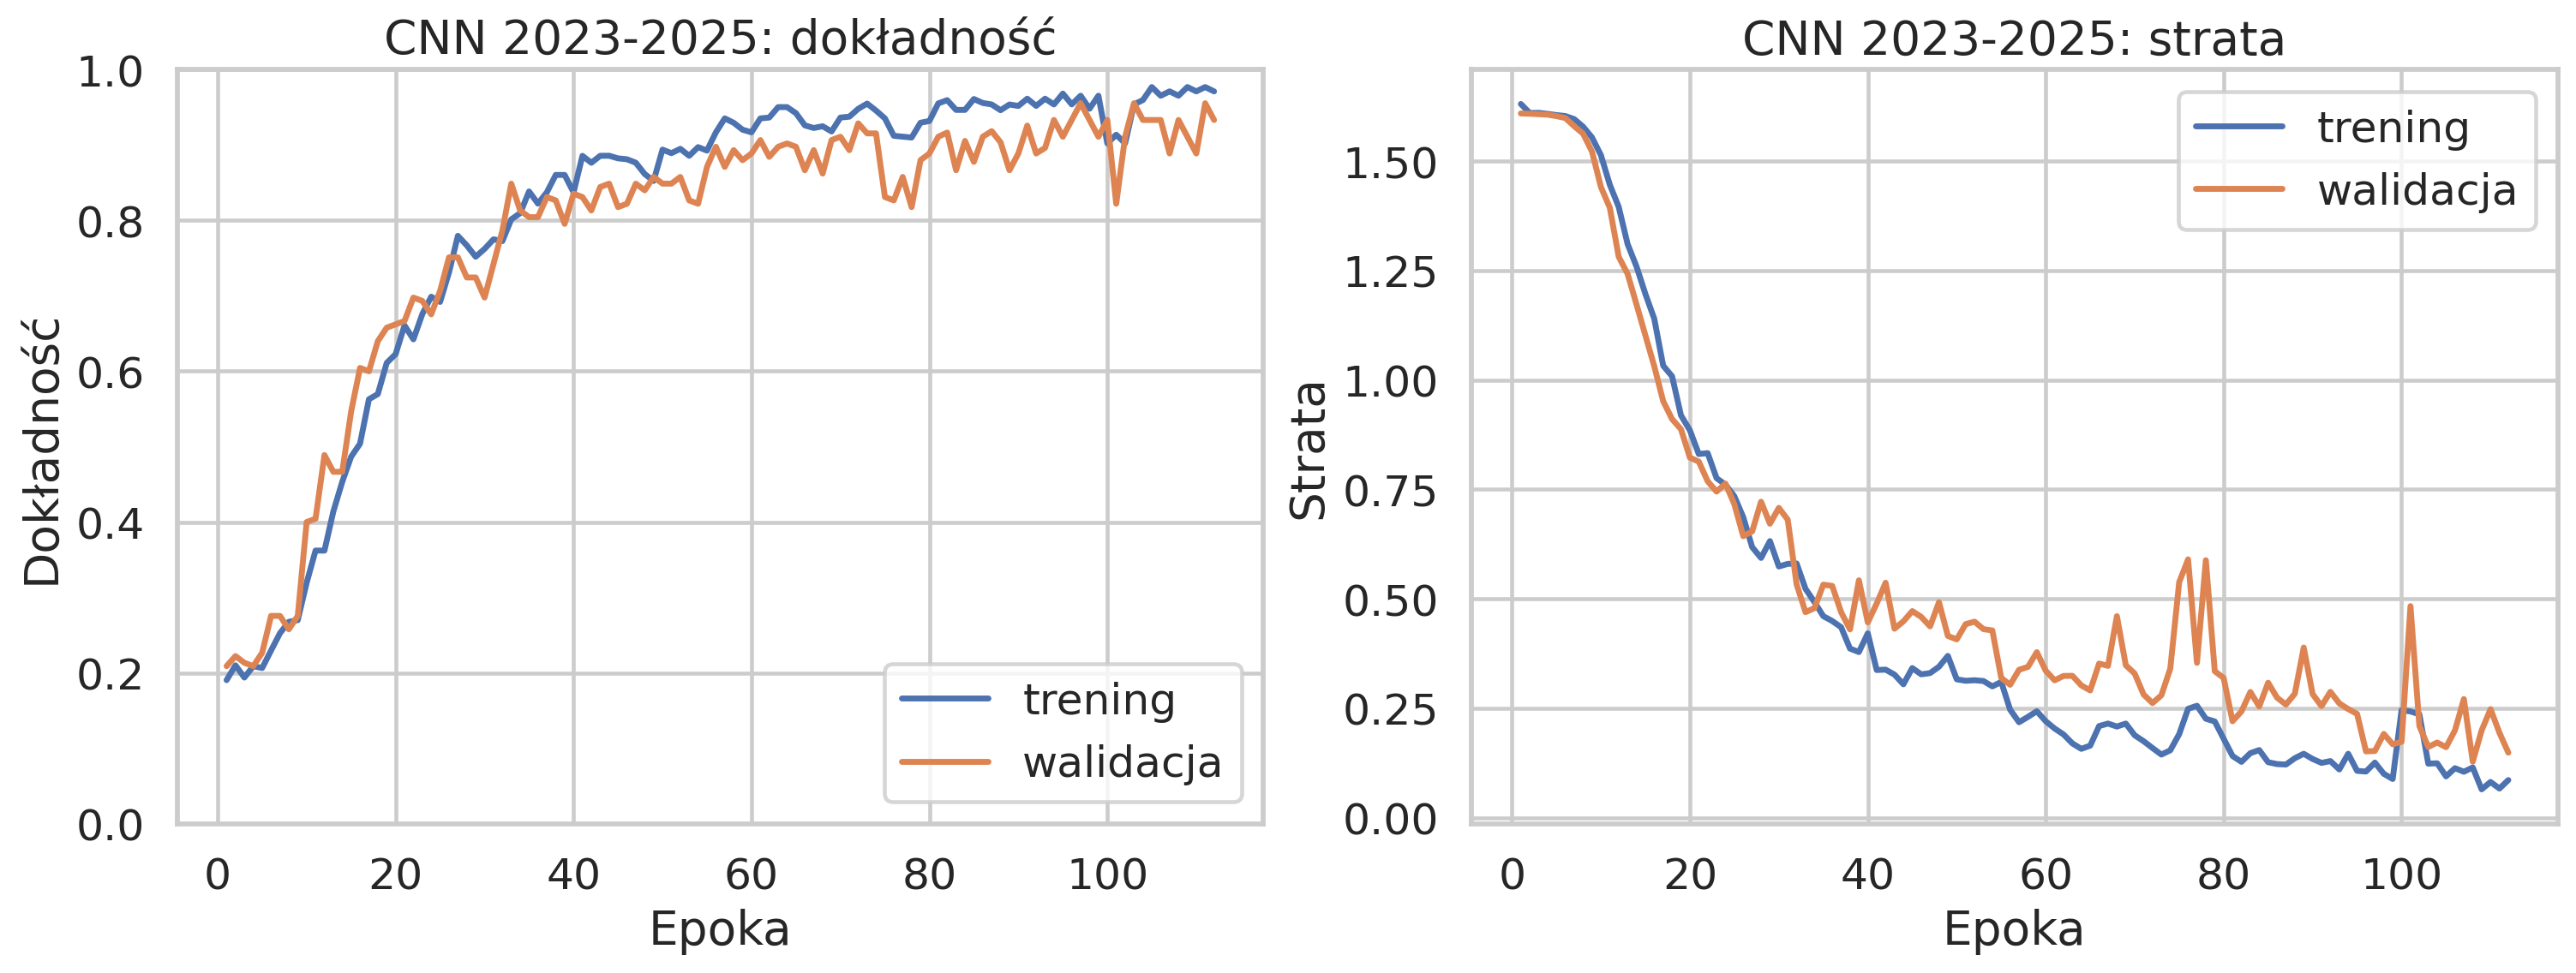
\includegraphics[width=0.90\textwidth]{03_cnn_training_curve_short_horizon.png}
\caption{Przykładowa krzywa uczenia modelu CNN w krótkim setupie kwalifikacyjnym.}
\label{fig:cnn-training-short}
\end{figure}

Lepszy wynik \texttt{CNN} jest spójny z podejściem, w którym zachowanie kierowcy traktuje się jako problem klasyfikacji szeregów czasowych \cite{hallac2016}. W takim ujęciu liczy się średnia wartość cechy oraz kształt fragmentu sygnału. W przypadku Formuły 1 może to oznaczać sekwencję obejmującą odjęcie gazu, hamowanie, redukcje biegów, minimalną prędkość i powrót na gaz. Model konwolucyjny może wychwycić takie lokalne wzorce bez konieczności ręcznego opisywania każdego zakrętu.

\section{Model hybrydowy CNN + cechy tabularne}

Następnie sprawdzono model hybrydowy, który łączył reprezentację sekwencyjną z ręcznie zdefiniowanymi cechami tabularnymi. Przyjęto założenie, że \texttt{CNN} może wychwycić lokalne wzorce przebiegu telemetrii, a cechy tabularne uzupełniają je o syntetyczne informacje o całym okrążeniu.

Ten wariant był najlepszy w krótkim setupie kwalifikacyjnym oraz w setupie wyścigowym. W kwalifikacjach 2023--2025 uzyskał 0.9147 macro F1, przy średniej foldowej \(0.9147 \pm 0.0512\). W czystych okrążeniach wyścigowych 2025 uzyskał 0.8564 macro F1, przy średniej foldowej \(0.8626 \pm 0.1175\). Wyższe odchylenie standardowe w setupie wyścigowym wskazuje, że wynik jest bardziej zależny od tego, które sesje trafiły do folda testowego.

\begin{figure}[H]
\centering
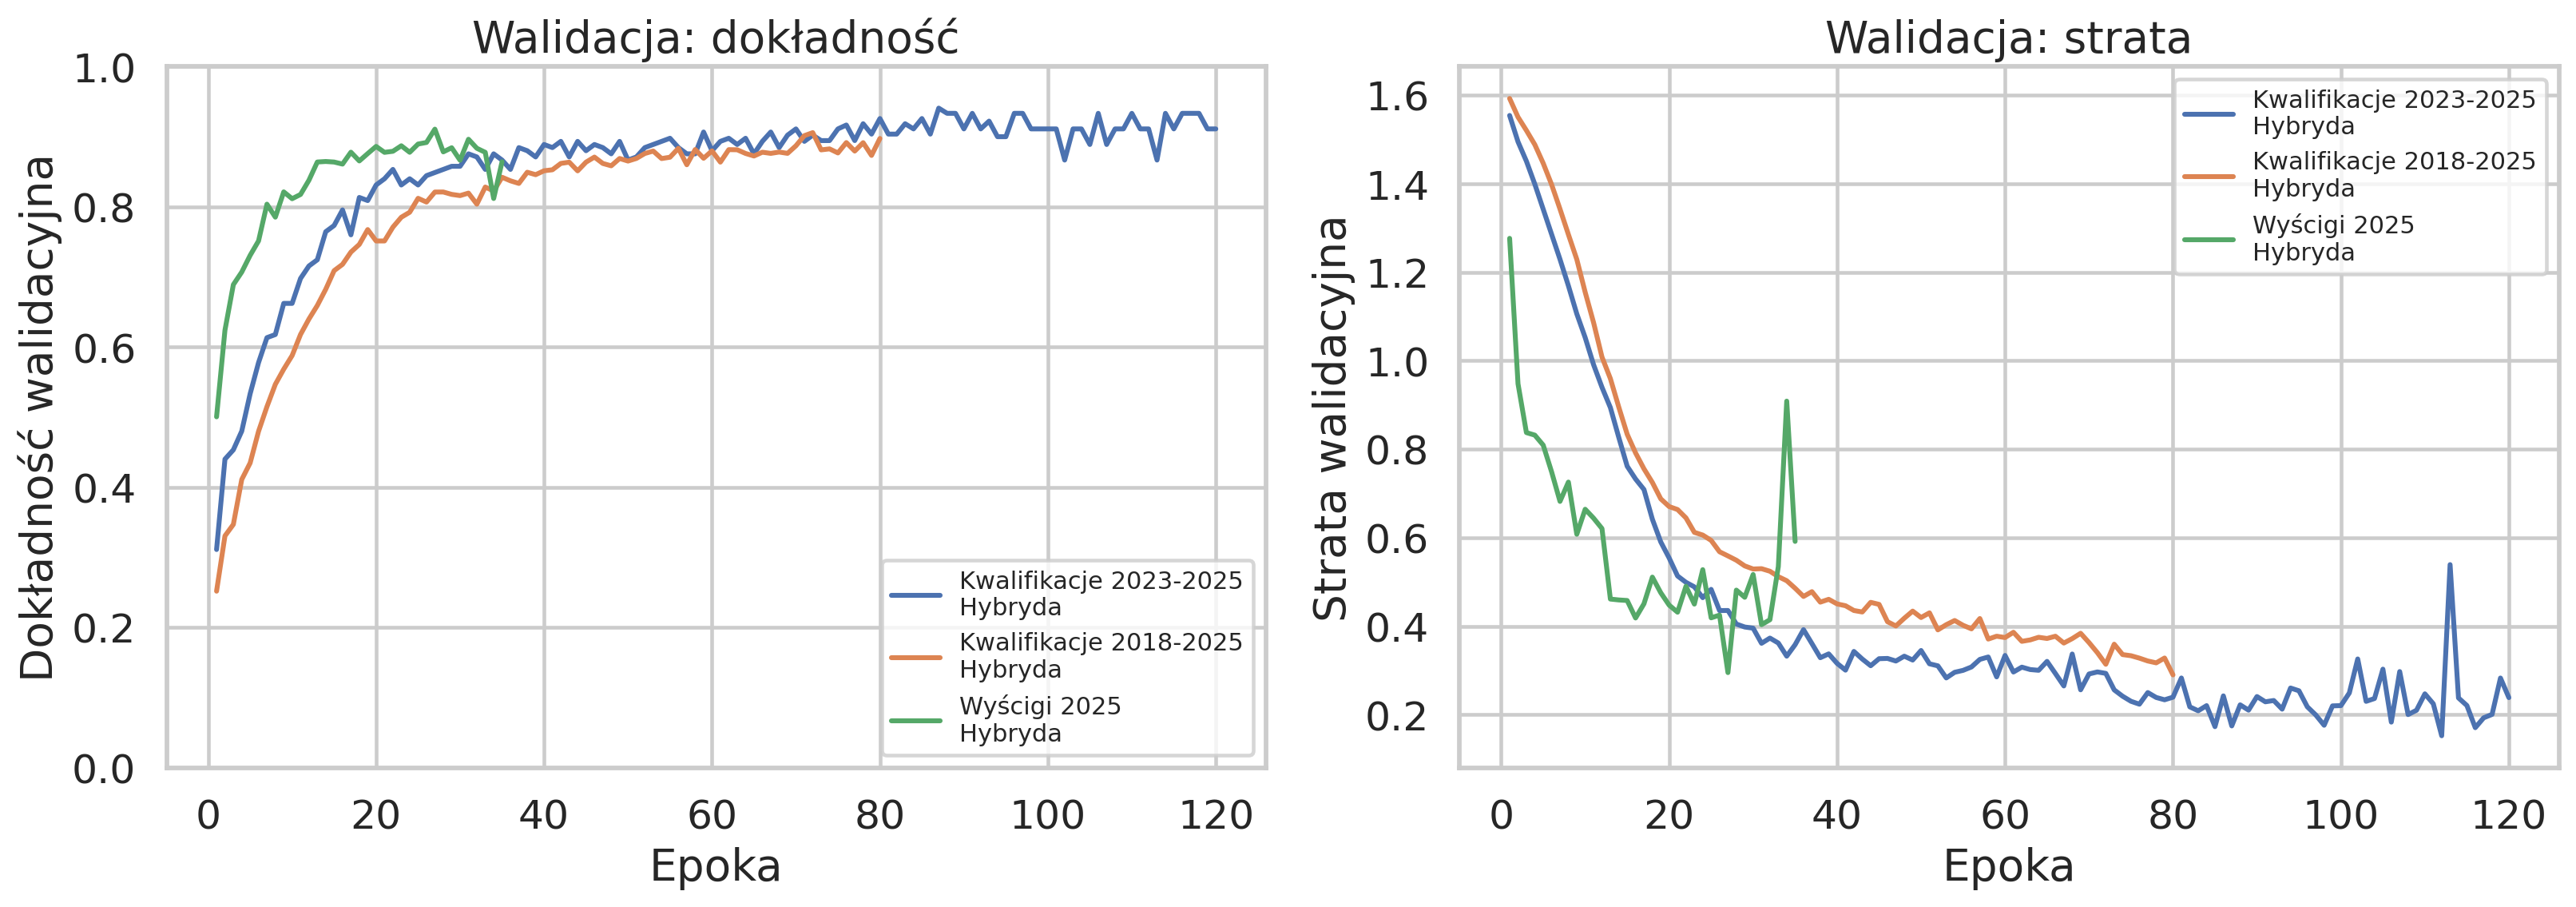
\includegraphics[width=0.95\textwidth]{10_training_curves_multisetup_hybrid.png}
\caption{Krzywe uczenia modelu hybrydowego w trzech setupach.}
\label{fig:training-curves}
\end{figure}

Na wykresie widać, że liczba faktycznie wykonanych epok różni się między setupami. Wynika to z użycia \emph{early stoppingu}. Modele miały ustalony maksymalny limit epok, a trening kończył się wcześniej, gdy wynik walidacyjny przestawał się poprawiać. Taka procedura ogranicza przeuczenie i pozwala porównywać modele według tej samej zasady zatrzymania, tego samego typu walidacji oraz wyniku na foldach testowych. Krótszy trening hybrydy w setupie wyścigowym oznacza, że model szybciej doszedł do najlepszego punktu walidacyjnego.

\begin{figure}[H]
\centering
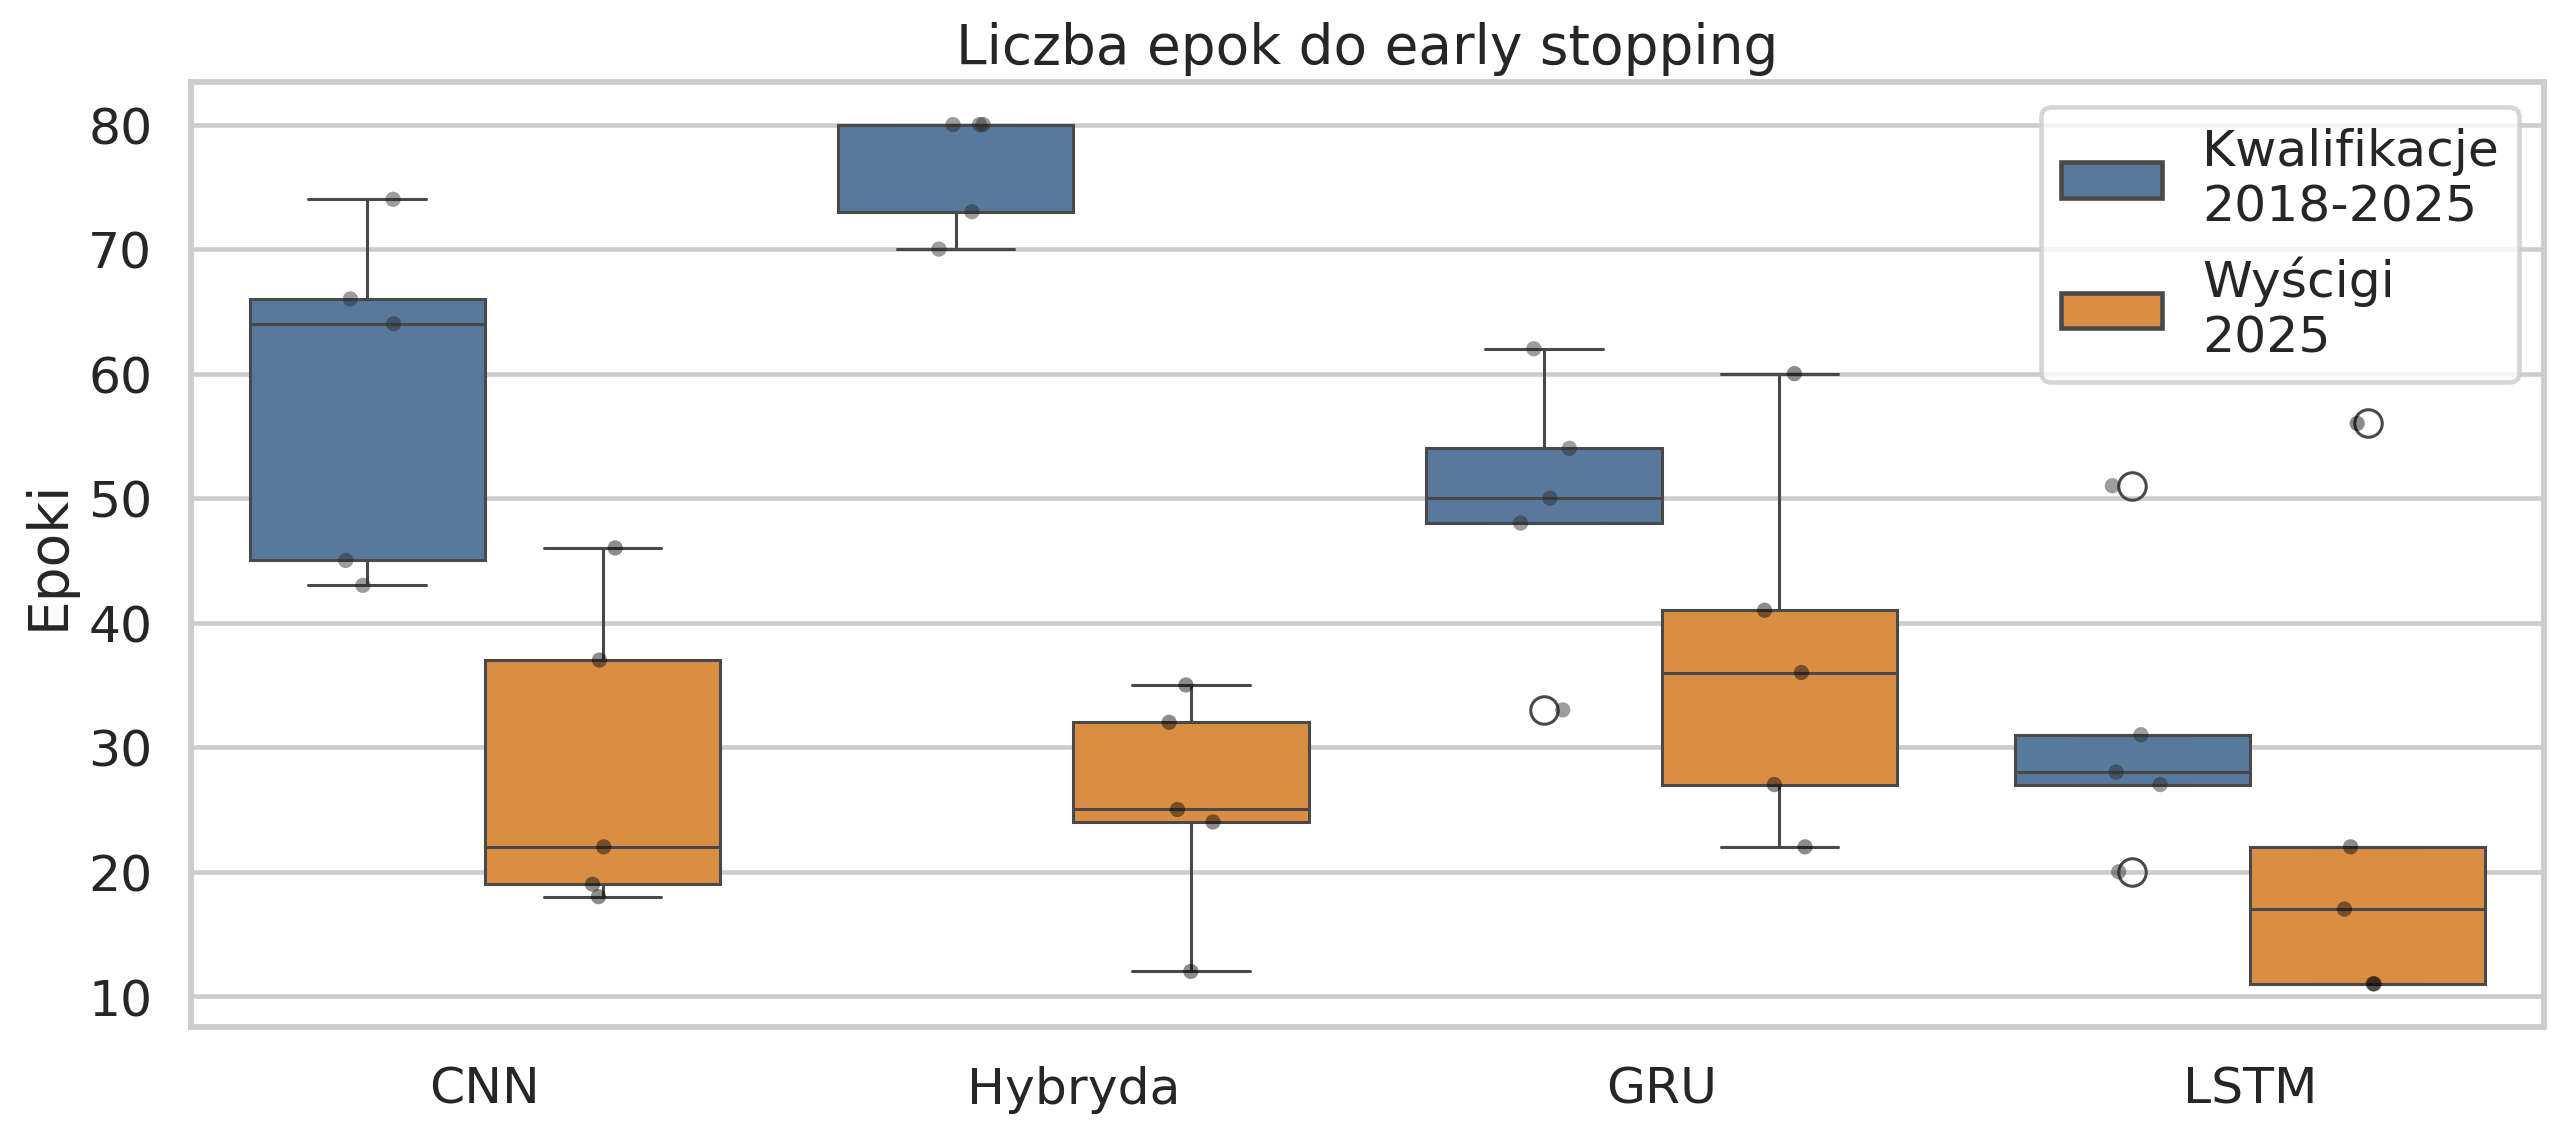
\includegraphics[width=0.85\textwidth]{04_epochs_to_early_stopping.png}
\caption{Liczba epok wykonanych przed zatrzymaniem treningu w modelach sekwencyjnych.}
\label{fig:epochs-early-stopping}
\end{figure}
\FloatBarrier

\section{GRU i LSTM}

Dla porównania sprawdzono również architektury rekurencyjne \texttt{GRU} i \texttt{LSTM}. Ich wyniki były wyraźnie słabsze od \texttt{CNN} i hybrydy. W krótkim setupie kwalifikacyjnym \texttt{GRU} uzyskał 0.4595 macro F1, a \texttt{LSTM} 0.3365 w predykcjach out-of-fold. W długim setupie kwalifikacyjnym oraz w setupie wyścigowym ich wyniki poprawiały się tylko częściowo i nie zmieniły ogólnego rankingu architektur.

Wyniki \texttt{GRU} i \texttt{LSTM} były bliskie poziomowi losowemu (dla pięciu zbalansowanych klas losowe macro F1 wynosi ok. 0.2). W połączeniu z faktem, że w krótkim i długim setupie kwalifikacyjnym modele rekurencyjne wypadały słabo mimo zwiększenia liczby danych, wskazuje to raczej na trudność optymalizacji tych architektur w przyjętej konfiguracji (sekwencja długości 300, niewielka próbka, ten sam optymalizator i kryterium zatrzymania co dla \texttt{CNN}, bez strojenia dedykowanego modelom rekurencyjnym) niż na ich zasadniczą nieprzydatność do problemu. Z tego powodu wniosek ograniczono do stwierdzenia, że w tej konkretnej reprezentacji i konfiguracji treningu architektury konwolucyjne okazały się skuteczniejsze i stabilniejsze od rekurencyjnych. Pełniejsze porównanie wymagałoby między innymi skrócenia sekwencji, zastosowania wariantów dwukierunkowych, przycinania gradientu oraz osobnego doboru kroku uczenia i kryterium early stopping dla \texttt{GRU} i \texttt{LSTM}.

\section{Zestawienie końcowe modeli}

Tabela~\ref{tab:model-results} przedstawia najważniejsze wyniki dla trzech setupów. W każdej komórce podano najpierw wynik macro F1 out-of-fold, a w drugiej linii średnią i odchylenie standardowe macro F1 na foldach testowych. Szczegółową niepewność wyników najlepszych modeli podano osobno w tabeli~\ref{tab:best-model-uncertainty}.

\begin{table}[H]
\centering
\scriptsize
\begin{tabularx}{\textwidth}{p{2.8cm}*{5}{>{\centering\arraybackslash}X}}
\toprule
Setup & Reg. log. & CNN & Hybryda & GRU & LSTM \\
\midrule
Kwalifikacje 2023--2025 &
\(\substack{0.8617\\0.8608\pm0.0193}\) &
\(\substack{0.8952\\0.8941\pm0.0479}\) &
\(\substack{\mathbf{0.9147}\\0.9147\pm0.0512}\) &
\(\substack{0.4595\\0.4445\pm0.0615}\) &
\(\substack{0.3365\\0.3170\pm0.1104}\) \\
Kwalifikacje 2018--2025 &
\(\substack{0.8267\\0.8262\pm0.0317}\) &
\(\substack{\mathbf{0.9012}\\0.9011\pm0.0264}\) &
\(\substack{0.8887\\0.8877\pm0.0345}\) &
\(\substack{0.2880\\0.2763\pm0.0129}\) &
\(\substack{0.2998\\0.2803\pm0.0516}\) \\
Wyścigi 2025 &
\(\substack{0.8177\\0.8243\pm0.0917}\) &
\(\substack{0.8466\\0.8589\pm0.0646}\) &
\(\substack{\mathbf{0.8564}\\0.8626\pm0.1175}\) &
\(\substack{0.5639\\0.5522\pm0.1584}\) &
\(\substack{0.3216\\0.2975\pm0.0731}\) \\
\bottomrule
\end{tabularx}
\caption{Macro F1 dla głównych rodzin modeli. W każdej komórce: wynik out-of-fold oraz średnia \(\pm\) odchylenie standardowe po foldach testowych.}
\label{tab:model-results}
\end{table}

Tabela~\ref{tab:model-results} pozwala porównać ranking rodzin modeli oraz podstawową zmienność wyników między foldami. Bootstrapowe przedziały ufności dla najlepszych modeli zebrano w tabeli~\ref{tab:best-model-uncertainty}, a porównania parowane w tabeli~\ref{tab:paired-model-comparisons}. Należy też zaznaczyć, że zestaw kierowców nie jest identyczny we wszystkich setupach (w krótkich kwalifikacjach występuje ALB, a w pozostałych setupach HAM), dlatego porównania między setupami dotyczą raczej trendu i rankingu architektur niż bezwzględnych wartości macro F1.

Najlepsze modele z każdego setupu zestawiono dodatkowo z bootstrapowym przedziałem ufności wyznaczonym na wynikach foldów testowych. Przy pięciu foldach taki przedział stanowi przybliżenie niepewności eksperymentu i pokazuje, jak stabilny był wynik końcowy w poszczególnych setupach.

\begin{table}[H]
\centering
\small
\begin{tabular}{lccc}
\toprule
Setup & Najlepszy model & OOF macro F1 & Fold mean $\pm$ std; 95\% CI \\
\midrule
Kwalifikacje 2023--2025 & Hybryda & 0.9147 & 0.9147 $\pm$ 0.0512; [0.8720, 0.9524] \\
Kwalifikacje 2018--2025 & CNN & 0.9012 & 0.9011 $\pm$ 0.0264; [0.8815, 0.9207] \\
Wyścigi 2025 & Hybryda & 0.8564 & 0.8626 $\pm$ 0.1175; [0.7570, 0.9357] \\
\bottomrule
\end{tabular}
\caption{Niepewność wyników dla najlepszych modeli w trzech setupach.}
\label{tab:best-model-uncertainty}
\end{table}

\begin{figure}[H]
\centering
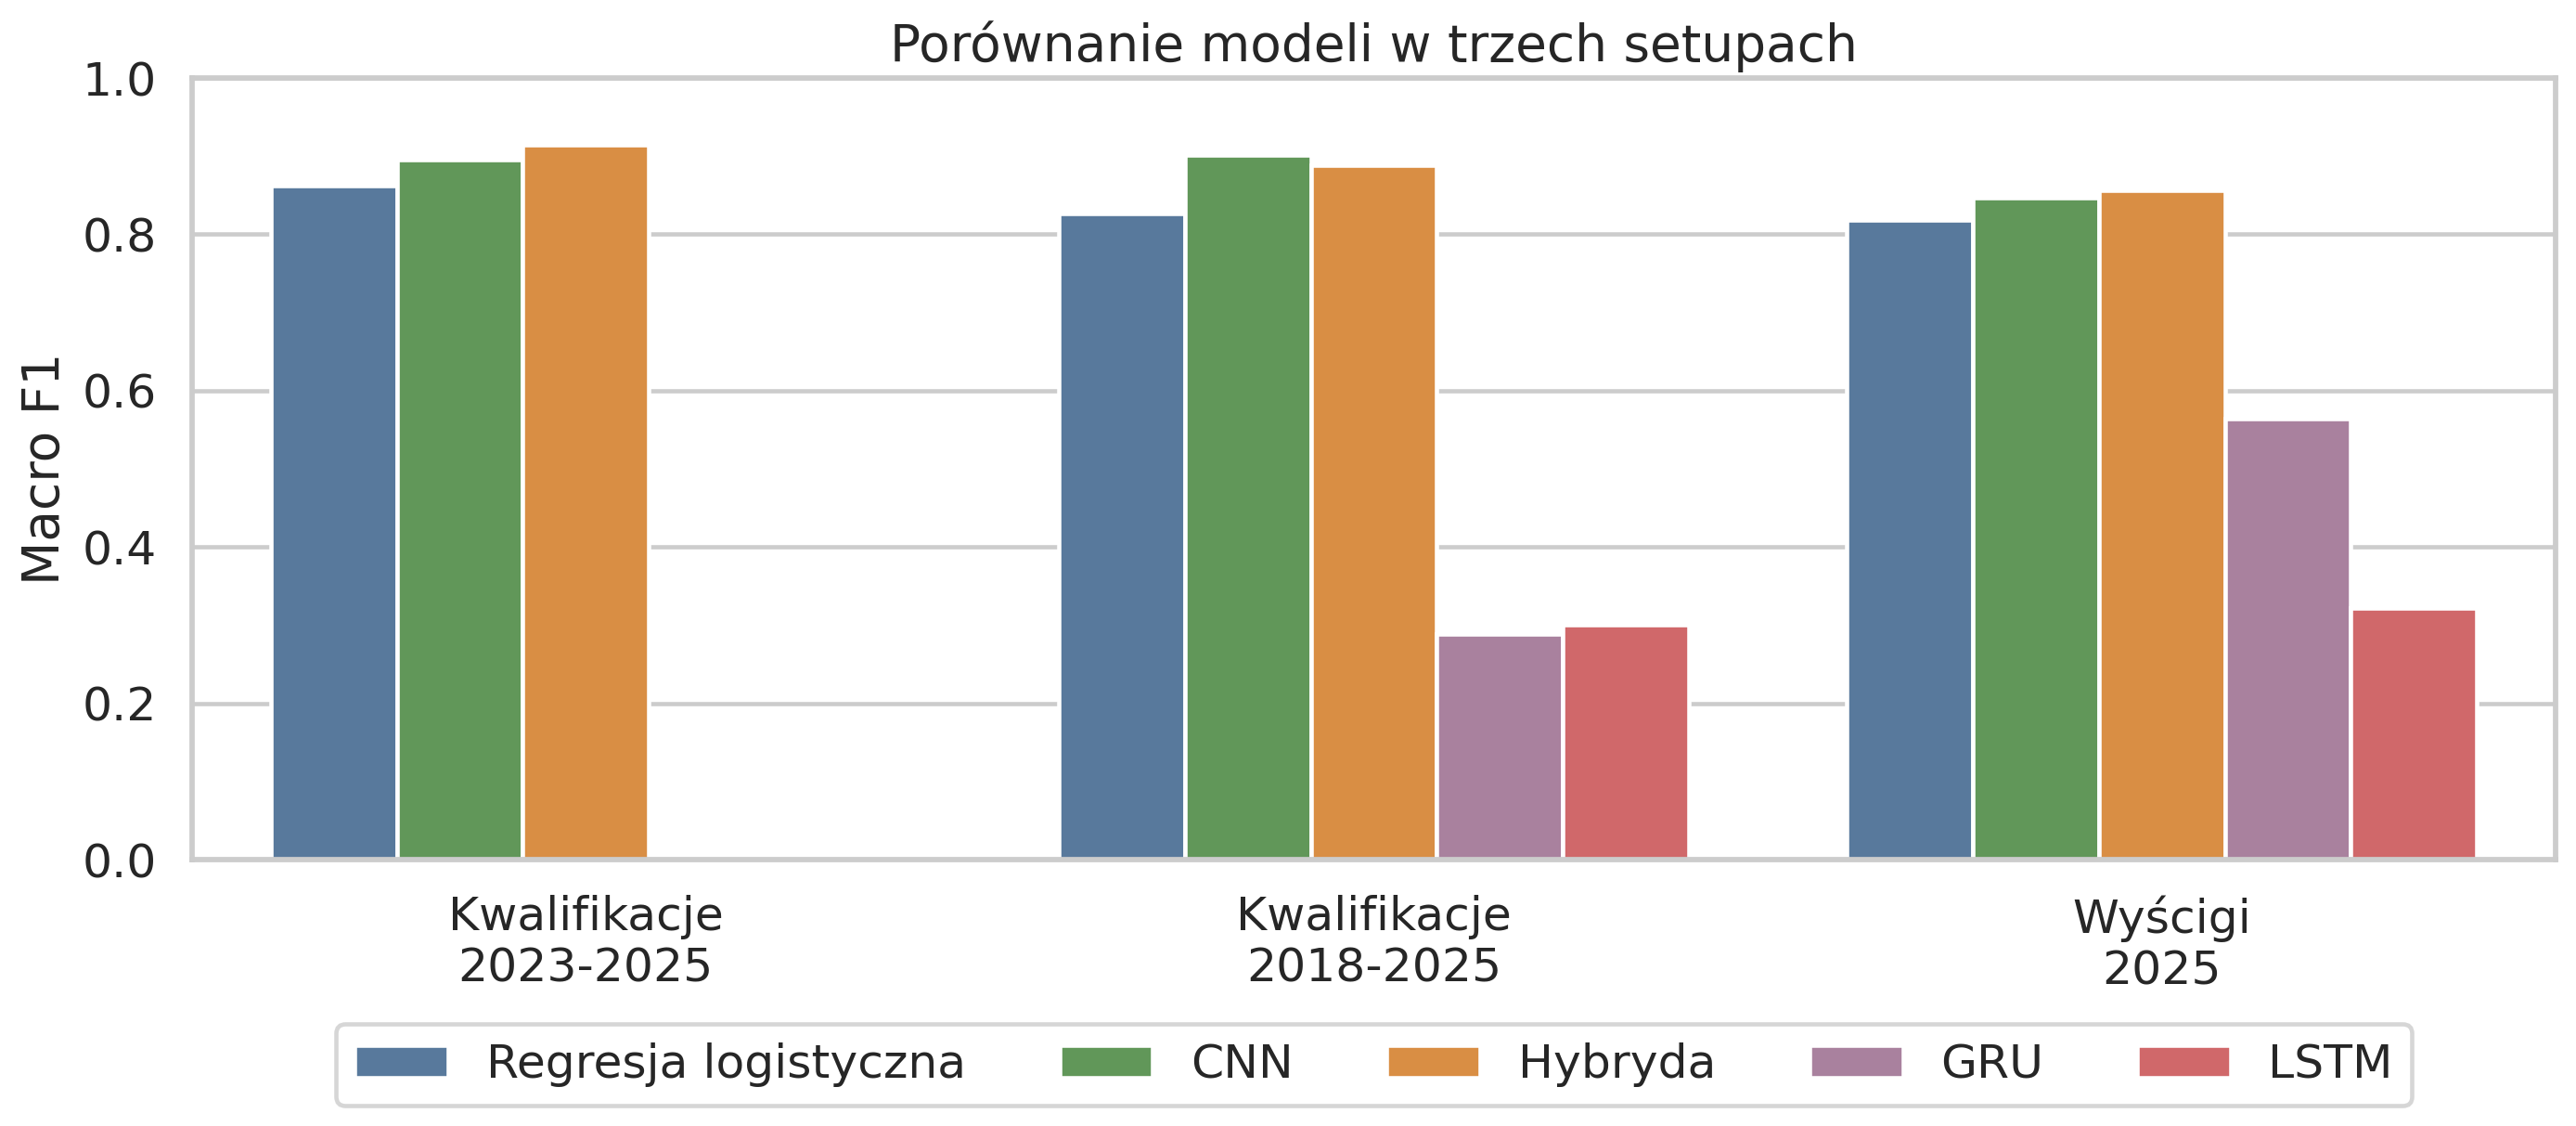
\includegraphics[width=0.95\textwidth]{02_model_progression.png}
\caption{Porównanie wyników modeli w trzech setupach.}
\label{fig:model-progression}
\end{figure}

Identyfikacja kierowcy na podstawie telemetrii okazała się możliwa we wszystkich trzech setupach. Najwyższe wyniki osiągały modele sekwencyjne i hybrydowe, co sugeruje, że pełny przebieg okrążenia zawiera dodatkową informację względem samych cech zagregowanych. Dla pięciu zbalansowanych klas losowy poziom macro F1 wynosi około 0.2, więc wszystkie modele tabularne, konwolucyjne i hybrydowe działały znacznie powyżej przypadku losowego; istotne różnice pojawiały się dopiero między rodzinami modeli, a nie względem poziomu odniesienia.

Wynik ten można zestawić z projektem WithSeismic, w którym opisano identyfikację kierowców F1 na podstawie dużej liczby fragmentów zakrętów \cite{withseismic2026}. Uzyskany tam wynik był istotnie lepszy od losowego i niższy niż w prezentowanej analizie. Eksperymenty różnią się źródłem danych, definicją próbki i podziałem problemu, ponieważ WithSeismic analizuje fragmenty zakrętów, a tutaj klasyfikowane są pełne okrążenia w wybranych setupach. Oba podejścia prowadzą jednak do podobnego wniosku, że telemetria zawiera mierzalny ślad kierowcy, a jakość wyniku zależy od definicji próbki, liczby klas i sposobu walidacji.

\begin{figure}[H]
\centering
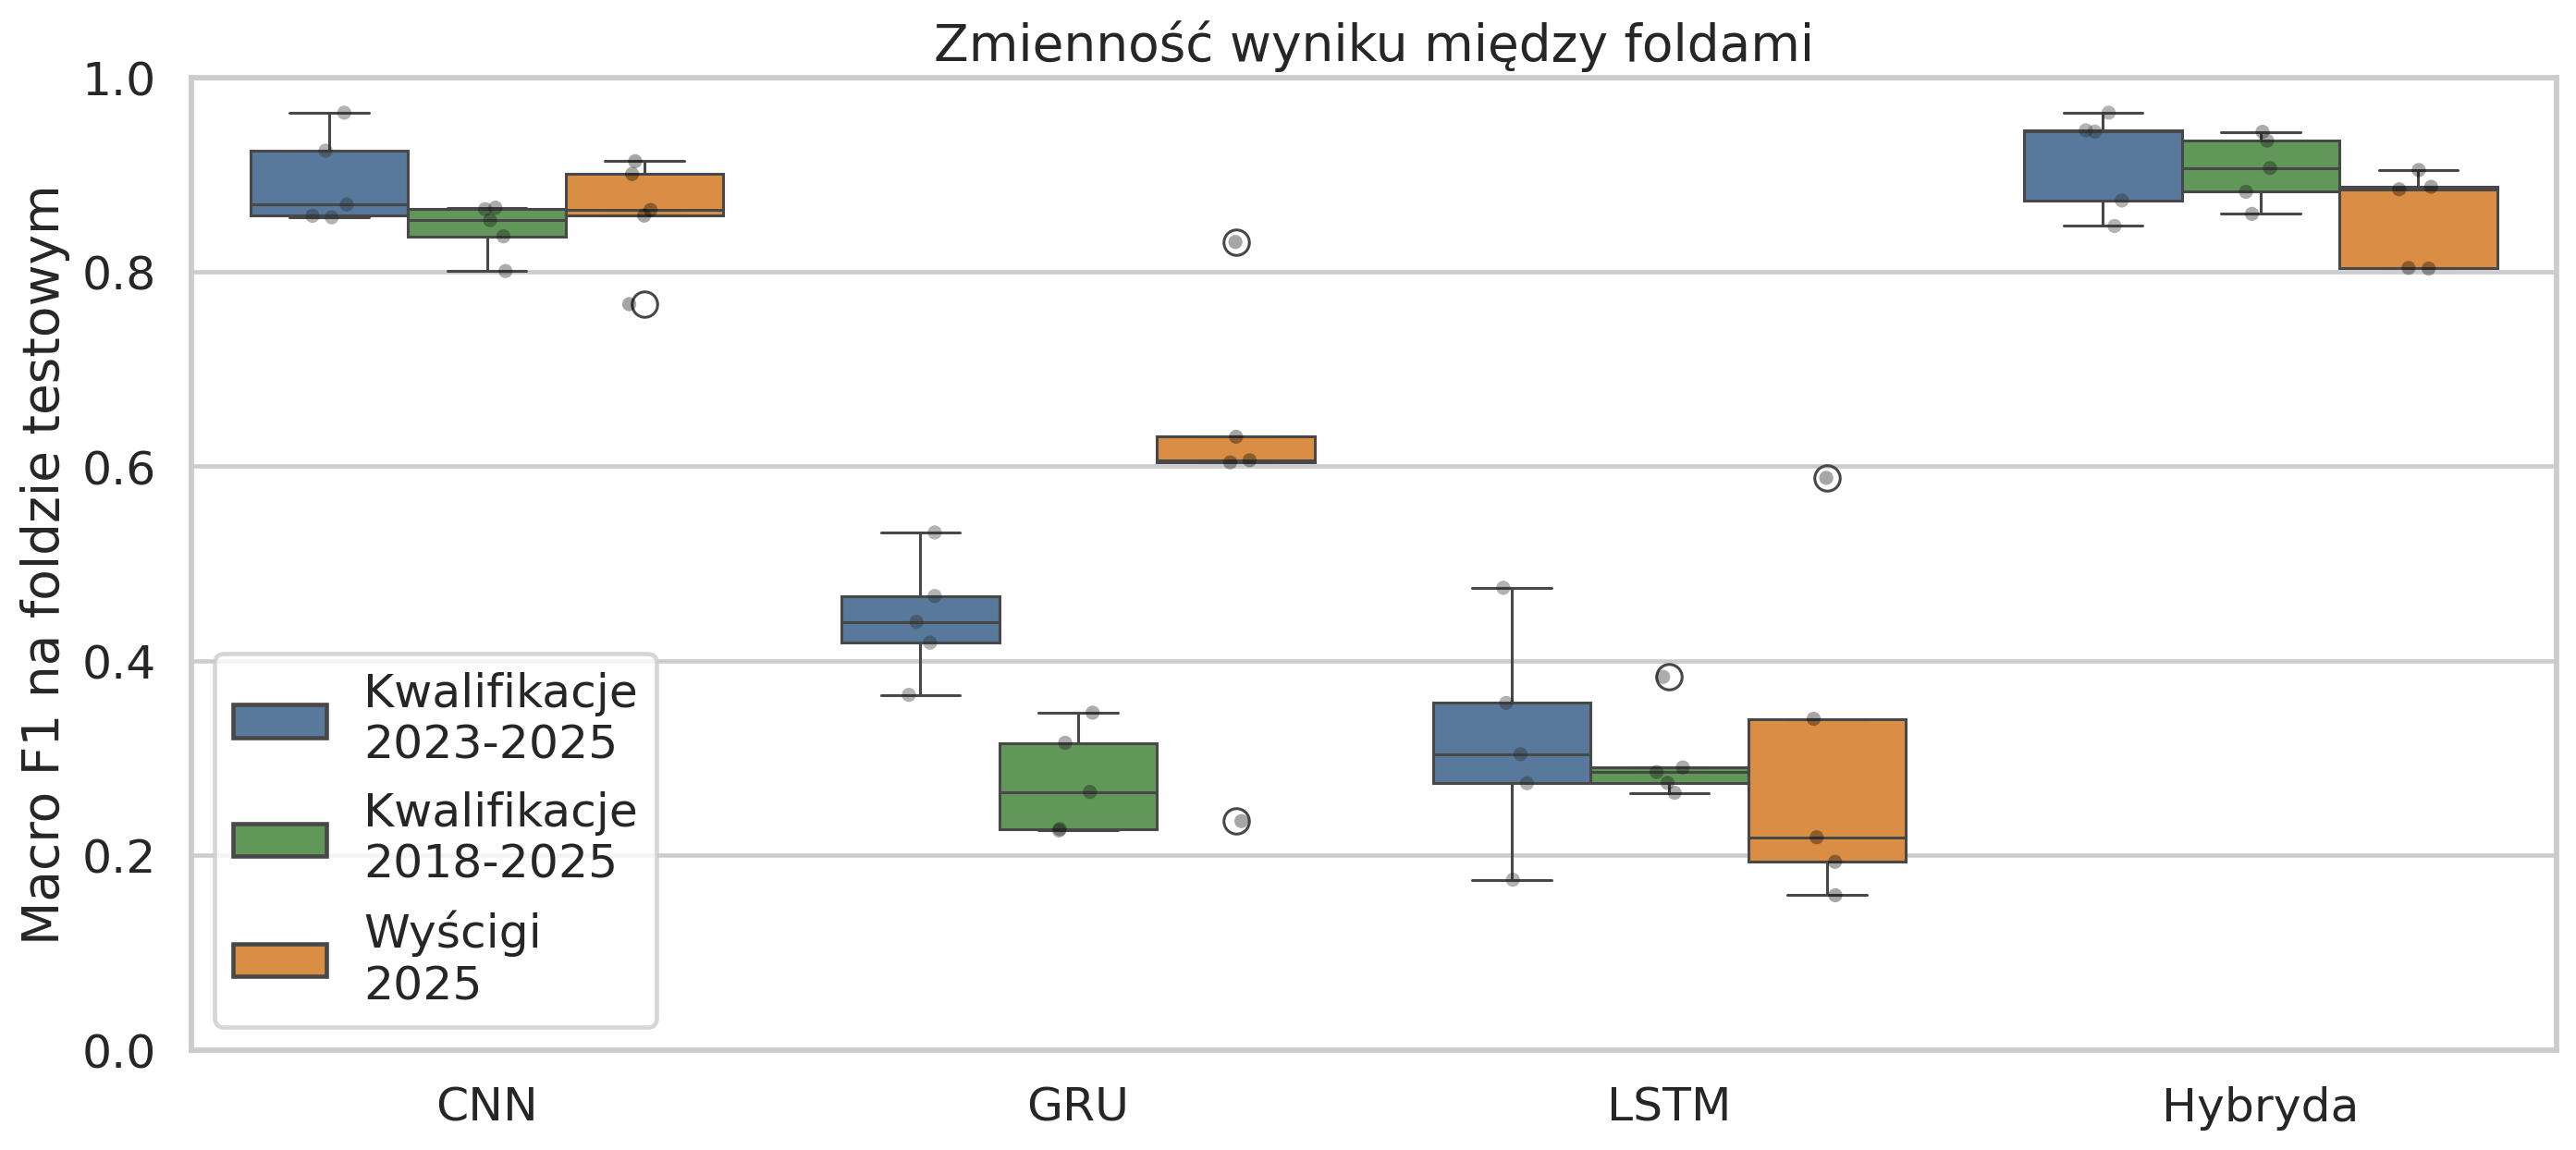
\includegraphics[width=0.95\textwidth]{11_sequence_fold_variability.png}
\caption{Zmienność wyniku między foldami walidacji.}
\label{fig:fold-variability}
\end{figure}

Wyniki między foldami pokazują, że jakość modelu zależy od konkretnego podziału sesji, ale ogólny ranking architektur pozostaje spójny. Najlepiej wypadają modele \texttt{CNN} i hybrydowe, natomiast \texttt{GRU} i \texttt{LSTM} są słabsze. Porównania parowane po foldach wzmacniają ten obraz, ale nie powinny być interpretowane zbyt kategorycznie ze względu na małą liczbę foldów.

\begin{table}[H]
\centering
\small
\begin{tabular}{lccc}
\toprule
Setup & Porównanie & Średnia różnica & Foldy dodatnie \\
\midrule
Kwalifikacje 2023--2025 & Hybryda -- regresja logistyczna & 0.0539 $\pm$ 0.0618 & 3/5 \\
Kwalifikacje 2018--2025 & CNN -- regresja logistyczna & 0.0749 $\pm$ 0.0413 & 5/5 \\
Wyścigi 2025 & Hybryda -- regresja logistyczna & 0.0382 $\pm$ 0.0902 & 3/5 \\
\bottomrule
\end{tabular}
\caption{Parowane porównania najlepszych modeli sekwencyjnych lub hybrydowych względem regresji logistycznej.}
\label{tab:paired-model-comparisons}
\end{table}

Najbardziej jednoznaczna przewaga pojawiła się w długim setupie kwalifikacyjnym, gdzie \texttt{CNN} był lepszy od regresji logistycznej we wszystkich pięciu foldach. W krótkim setupie i w setupie wyścigowym przewaga modeli sekwencyjnych była mniej stabilna fold po foldzie, mimo lepszych wyników średnich i out-of-fold. Wyniki te wspierają wybór \texttt{CNN} i hybrydy jako najmocniejszych architektur, a jednocześnie pokazują znaczenie raportowania niepewności różnic między modelami.

\section{Macierze pomyłek}

Macierze pomyłek najlepszych modeli pokazano na rysunku~\ref{fig:sequence-confusion}.

\begin{figure}[H]
\centering
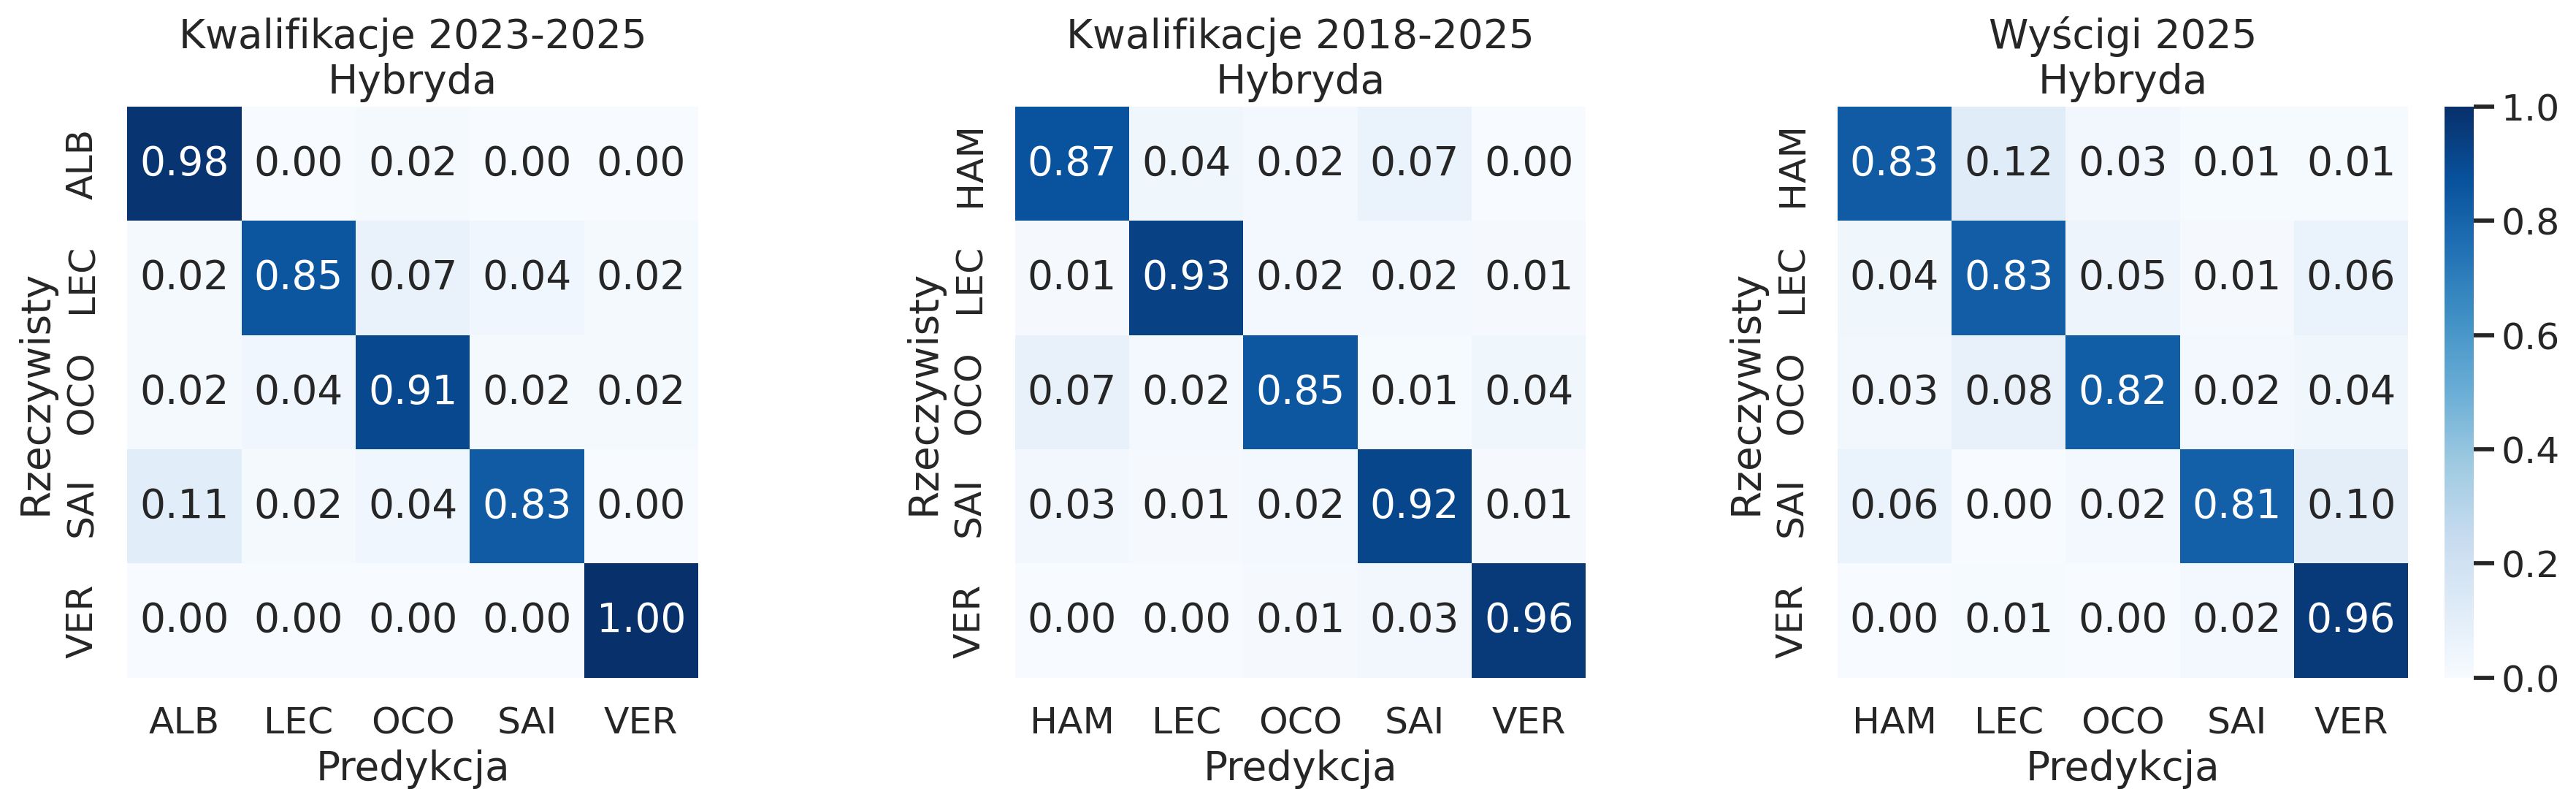
\includegraphics[width=0.95\textwidth]{12_best_sequence_confusion_matrices.png}
\caption{Macierze pomyłek najlepszych modeli sekwencyjnych i hybrydowych.}
\label{fig:sequence-confusion}
\end{figure}
\FloatBarrier

Macierze pomyłek pozwalają sprawdzić, którzy kierowcy są rozpoznawani najlepiej, a które pary są mylone; wysoki wynik globalny nie wystarcza, aby ocenić, czy model rozpoznaje każdego kierowcę z osobna. W krótkim setupie kwalifikacyjnym najpewniej rozpoznawany był Verstappen, a najwięcej pomyłek dotyczyło pary Albon--Sainz. W setupie wyścigowym 2025 najsilniejsza pomyłka pojawiała się natomiast między Hamiltonem a Leclerkiem, czyli kierowcami tego samego zespołu (Ferrari). Jest to spójne z wnioskami z Badania~2: gdy dwóch kierowców dzieli ten sam samochód, ich profile telemetryczne są do siebie bliższe, a zadanie klasyfikacji staje się trudniejsze. Pomyłki nie rozkładają się więc losowo, lecz koncentrują w obrębie podobnego sprzętu i zbliżonych warunków.

\section{Interpretacja cech}

Najważniejsze cechy modelu pokazano na rysunku~\ref{fig:feature-importance}.

\begin{figure}[H]
\centering
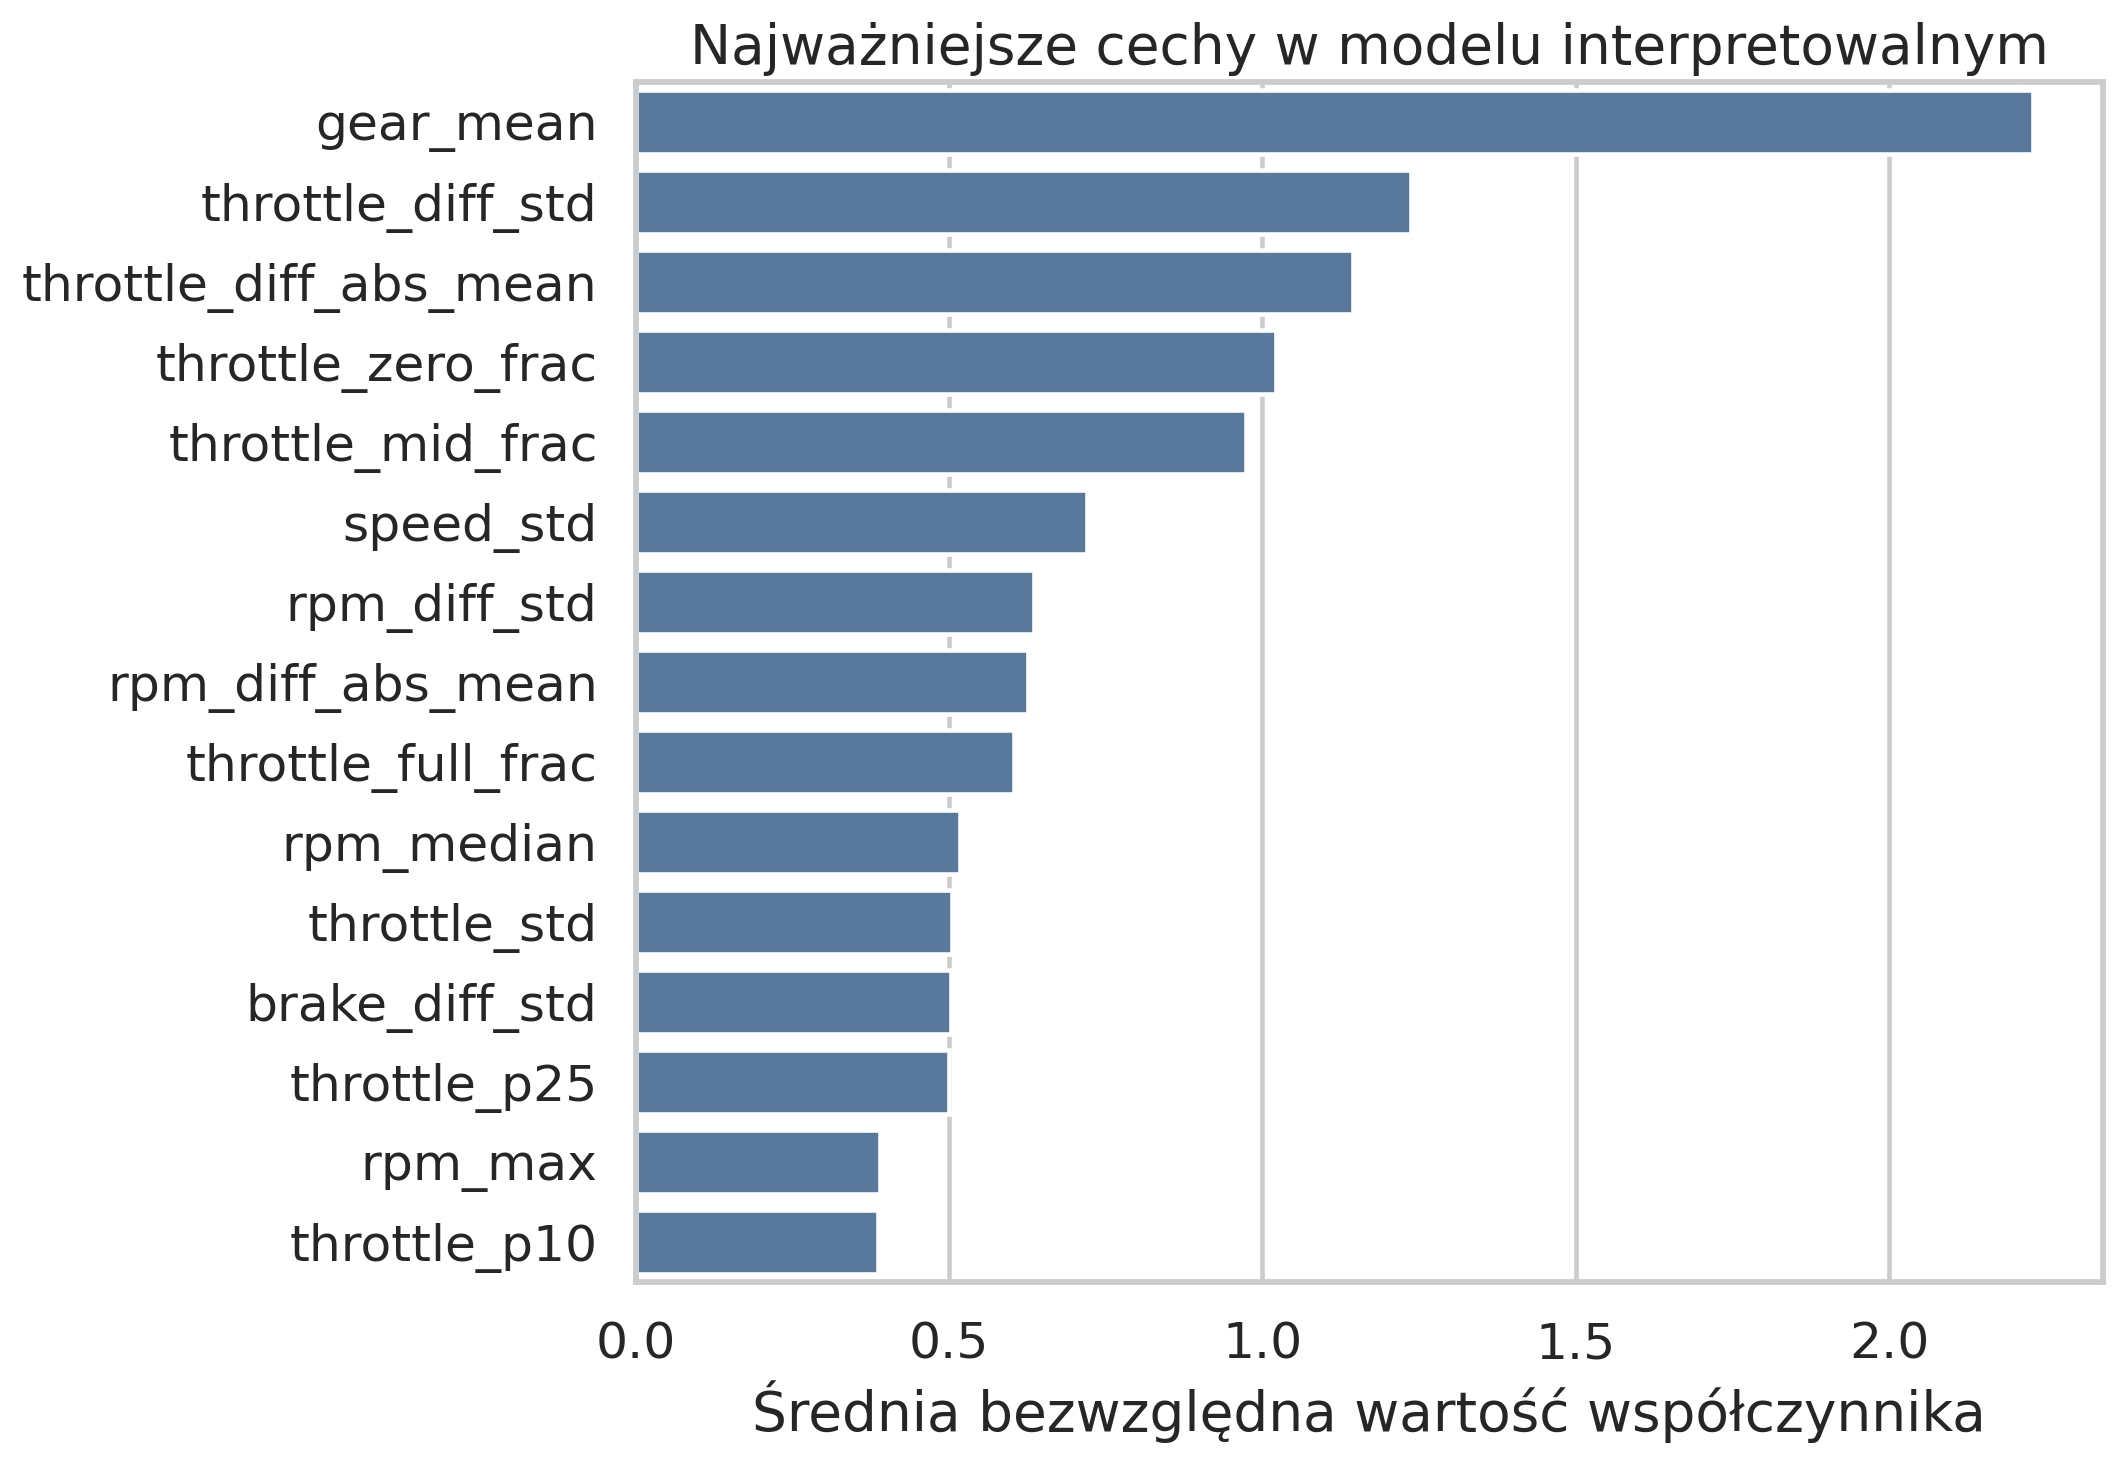
\includegraphics[width=0.85\textwidth]{06_driver_feature_importance.png}
\caption{Najważniejsze cechy w modelu interpretowalnym.}
\label{fig:feature-importance}
\end{figure}

Najważniejsze cechy modelu interpretowalnego dotyczą przede wszystkim operowania gazem, biegami, obrotami silnika, hamowaniem oraz dynamiką sygnałów. Wskazuje to na wykorzystanie informacji szerszej niż samo tempo okrążenia.

Interpretację współczynników regresji logistycznej uzupełniono analizą permutation importance. W tej procedurze wartości wybranej cechy albo całej rodziny cech są losowo permutowane w części testowej, a następnie mierzy się spadek jakości modelu. Wyraźny spadek wyniku po permutacji oznacza, że dana informacja była istotna dla klasyfikatora. Takie podejście sprawdza bezpośredni wpływ cechy na wynik predykcji i uzupełnia interpretację samych wag modelu.

\begin{table}[H]
\centering
\small
\begin{tabular}{lccccc}
\toprule
Setup & Gaz & Biegi & Obroty & Hamowanie & Prędkość \\
\midrule
Kwalifikacje 2023--2025 & 0.5455 & 0.2365 & 0.2240 & 0.2046 & 0.1043 \\
Kwalifikacje 2018--2025 & 0.4331 & 0.3447 & 0.3617 & 0.1875 & 0.3457 \\
Wyścigi 2025 & 0.4435 & 0.2916 & 0.2052 & 0.1854 & 0.2652 \\
\bottomrule
\end{tabular}
\caption{Spadek macro F1 po permutacji rodzin cech w modelu regresji logistycznej.}
\label{tab:permutation-family-importance}
\end{table}

Tabela~\ref{tab:permutation-family-importance} pokazuje, że największe znaczenie miały rodziny cech związane z przepustnicą, biegami, obrotami silnika i prędkością. Hamowanie również wnosiło informację, choć słabszą niż gaz i profil pracy układu napędowego. Jest to spójne z przeglądami rozpoznawania stylu jazdy, w których zachowanie kierowcy opisuje się między innymi przez przyspieszanie, hamowanie, prędkość i dynamikę manewrów \cite{driving_style_review}.

Wśród pojedynczych cech bardzo wysoko pojawiała się \texttt{gear\_mean}, czyli średni bieg używany w okrążeniu. W praktyce jest to skrót informacji o całym profilu przejazdu, obejmującym prędkości w zakrętach, momenty redukcji, długość faz przyspieszania, charakterystykę toru i sposób pracy samochodu. Taka cecha może pomagać w rozpoznawaniu kierowcy, a zarazem przenosić wpływ toru, sezonu i zespołu. Z tego powodu kolejne badanie poświęcono kontroli biasu zespołowego oraz dodatkowym testom kontekstowym.

W tej pracy warstwę interpretowalności oparto świadomie na współczynnikach regresji logistycznej oraz permutation importance liczonej dla rodzin cech, co jest spójne z wyborem regresji logistycznej jako głównego, interpretowalnego modelu tabularnego. Permutation importance ma jednak ograniczenia: przy silnie skorelowanych cechach spadek wyniku po permutacji może rozkładać się między kilka podobnych zmiennych, a sama metoda nie pokazuje kierunku zależności. Wyniki z tabeli wskazują więc rodziny sygnałów użytecznych dla modelu, lecz interpretacja przyczynowa wymagałaby dodatkowych analiz. Metody SHAP, partial dependence oraz lokalne wyjaśnienia pojedynczych okrążeń pozostawiono jako rozszerzenie ze względu na zakres pracy oraz wspomniane skorelowanie cech telemetrycznych, które utrudnia jednoznaczne przypisanie wkładu pojedynczej zmiennej.

\chapter{Badanie 2: Bias zespołowy i wpływ samochodu}

\section{Motywacja}

Wynik klasyfikacji kierowcy może być zawyżony, jeżeli model uczy się stylu kierowcy razem z charakterystyką samochodu lub zespołu. Dlatego w drugim badaniu sprawdzono, czy z tych samych danych można przewidywać zespół oraz czy predykcja zespołu pomaga w predykcji kierowcy.

\section{Predykcja kierowcy a predykcja zespołu}

Porównanie wyników predykcji kierowcy i zespołu przedstawiono na rysunku~\ref{fig:driver-vs-team}.

\begin{figure}[H]
\centering
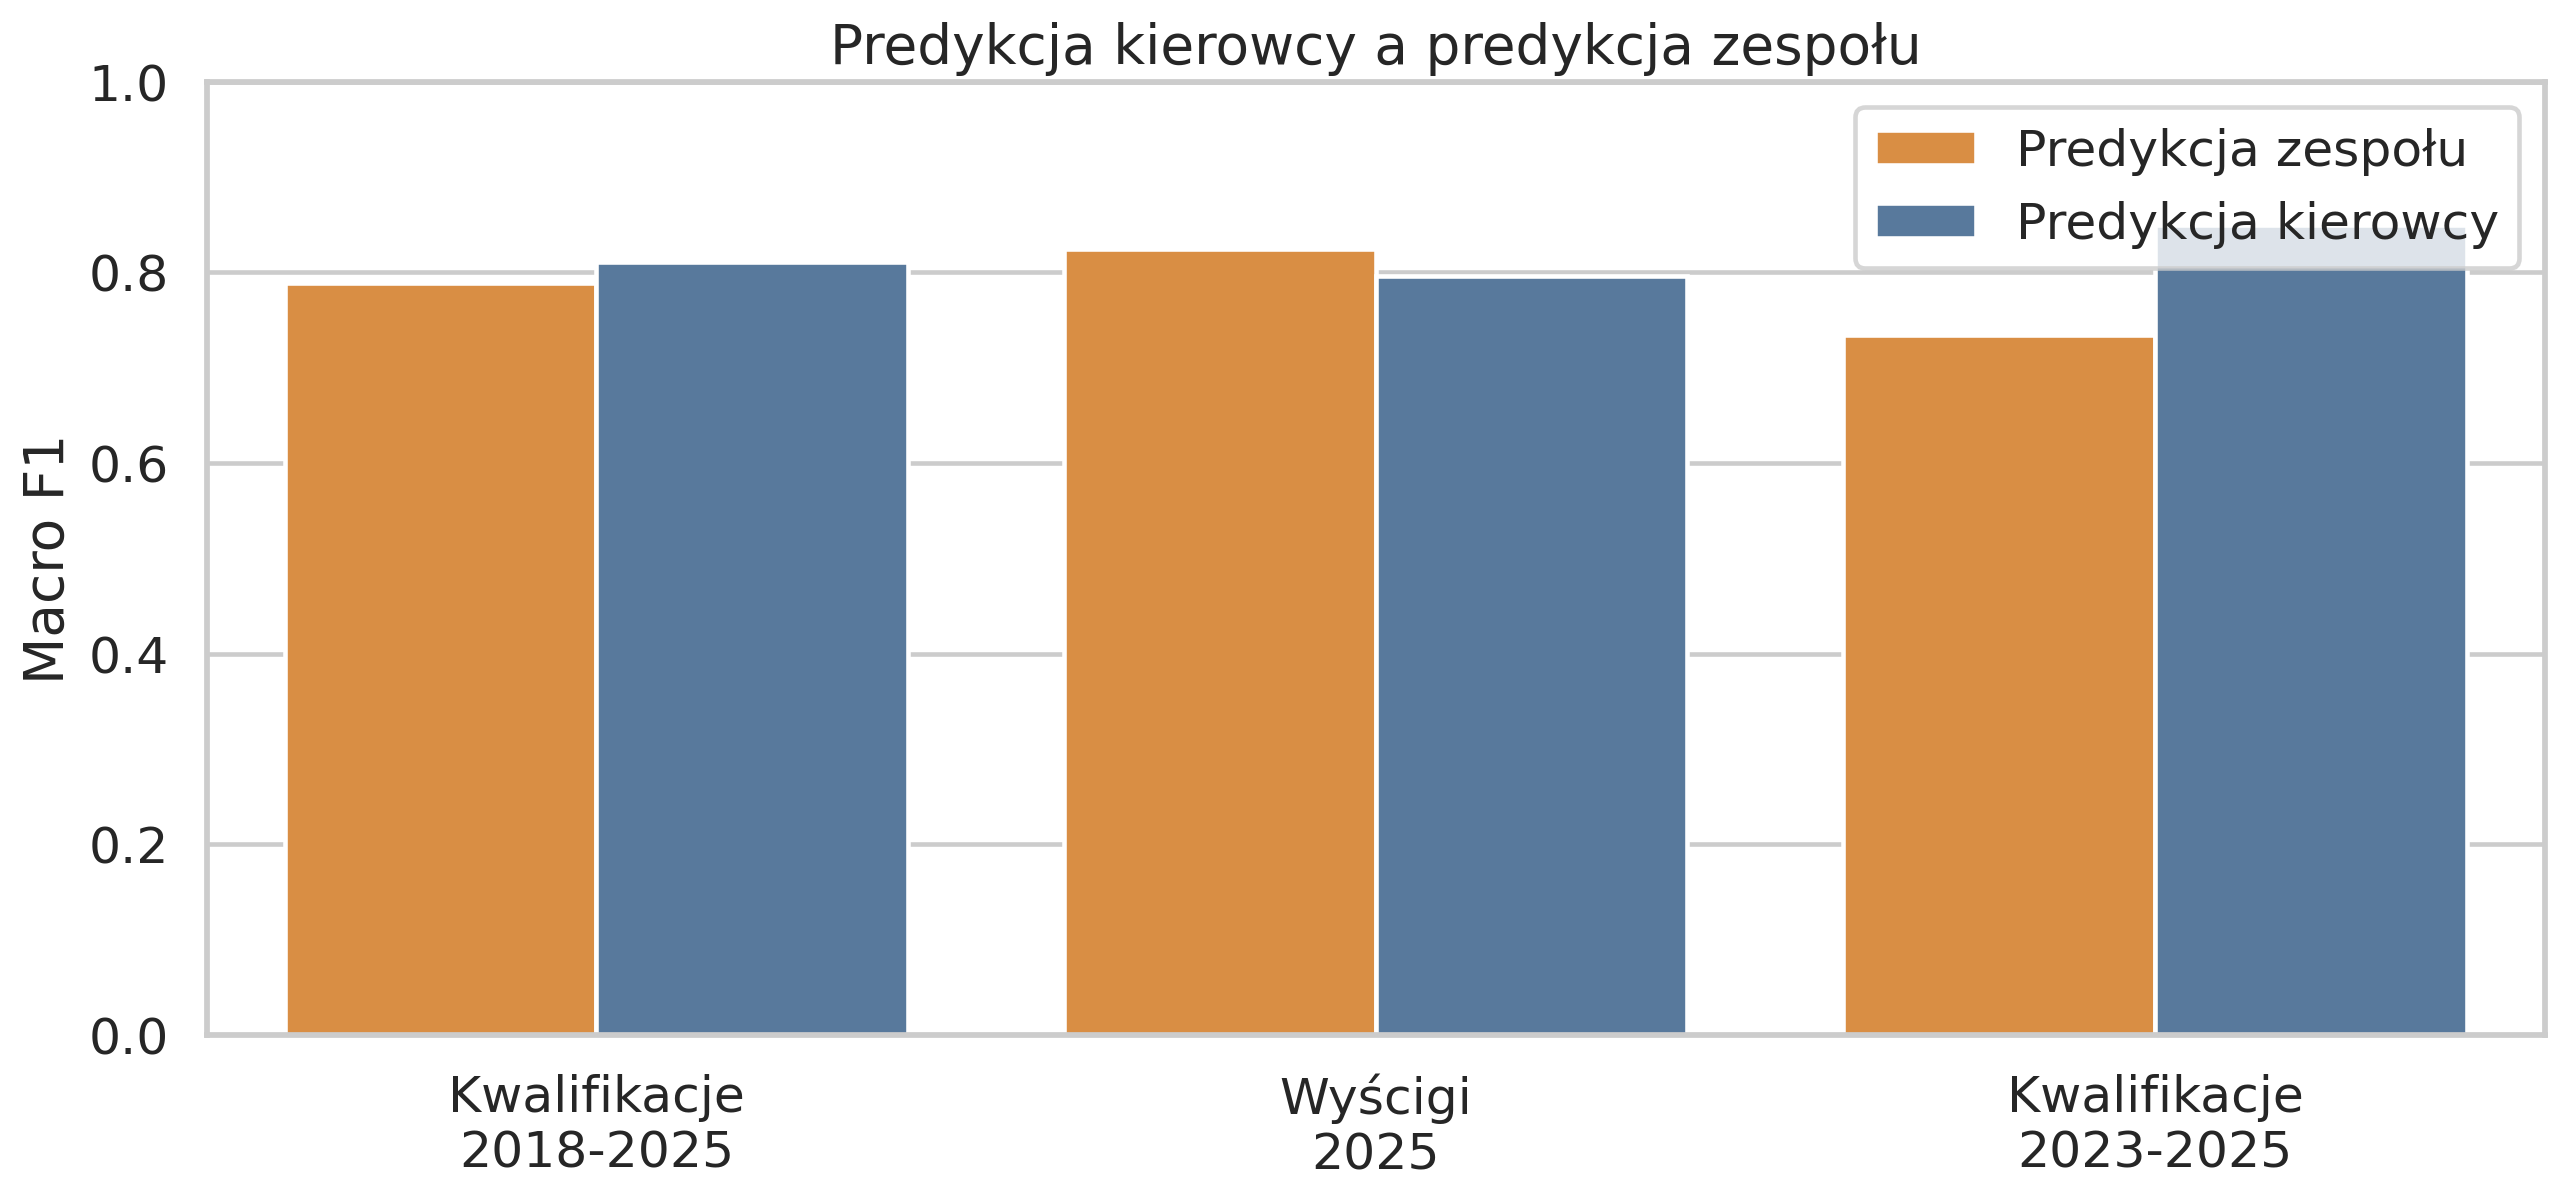
\includegraphics[width=0.90\textwidth]{07_driver_vs_team_prediction.png}
\caption{Porównanie predykcji kierowcy i predykcji zespołu.}
\label{fig:driver-vs-team}
\end{figure}

Zespół również ma wyraźny podpis telemetryczny. Oznacza to obecność realnego biasu zespołowego, którego nie można ignorować przy interpretacji modeli kierowcy. Predykcję zespołu sprawdzono także w wariantach bez bezpośrednich cech czasowych, aby nie sprowadzić zadania wyłącznie do rozpoznawania najszybszych i najwolniejszych samochodów.

\begin{table}[H]
\centering
\small
\begin{tabular}{lccc}
\toprule
Setup & Liczba klas zespołów & Konfiguracja cech & Macro F1 \\
\midrule
Kwalifikacje 2023--2025 & 8 & bez czasu i kontekstu & 0.7340 \\
Kwalifikacje 2018--2025 & 6 & bez czasu i kontekstu & 0.7884 \\
Wyścigi 2025 & 4 & wszystkie cechy telemetryczne & 0.8242 \\
\bottomrule
\end{tabular}
\caption{Najlepsze wyniki predykcji zespołu w analizie biasu zespołowego.}
\label{tab:team-prediction}
\end{table}

Intuicyjnie można oczekiwać, że zespół łatwo rozpoznać po czasie okrążenia lub prędkości maksymalnej. Dobre rezultaty pojawiały się jednak także po usunięciu cech czasowych. Oznacza to, że model wykrywał ogólne tempo oraz szerszy profil telemetryczny samochodu, obejmujący sposób osiągania prędkości, zakres pracy biegów, charakterystykę gazu i obrotów.

Ten element odróżnia analizę Formuły 1 od wielu klasycznych prac o identyfikacji kierowcy. W zwykłych danych drogowych często zakłada się stały lub drugorzędny wpływ samochodu. W F1 samochód i zespół są częścią problemu, ponieważ kierowcy prowadzą różne konstrukcje, a charakterystyka auta może wpływać na prędkość, dobór biegów i sposób oddawania mocy. Dlatego wysoki wynik identyfikacji kierowcy wymaga kontroli, czy model w praktyce nie rozpoznaje głównie samochodu.

\section{Model hierarchiczny i team-aware}

Sprawdzono dwa warianty wykorzystania informacji o zespole:

\begin{itemize}
    \item model hierarchiczny, w którym najpierw przewidywany jest zespół, a następnie kierowca;
    \item model team-aware, w którym prawdopodobieństwa zespołu są dodatkowymi cechami dla modelu kierowcy.
\end{itemize}

\begin{figure}[H]
\centering
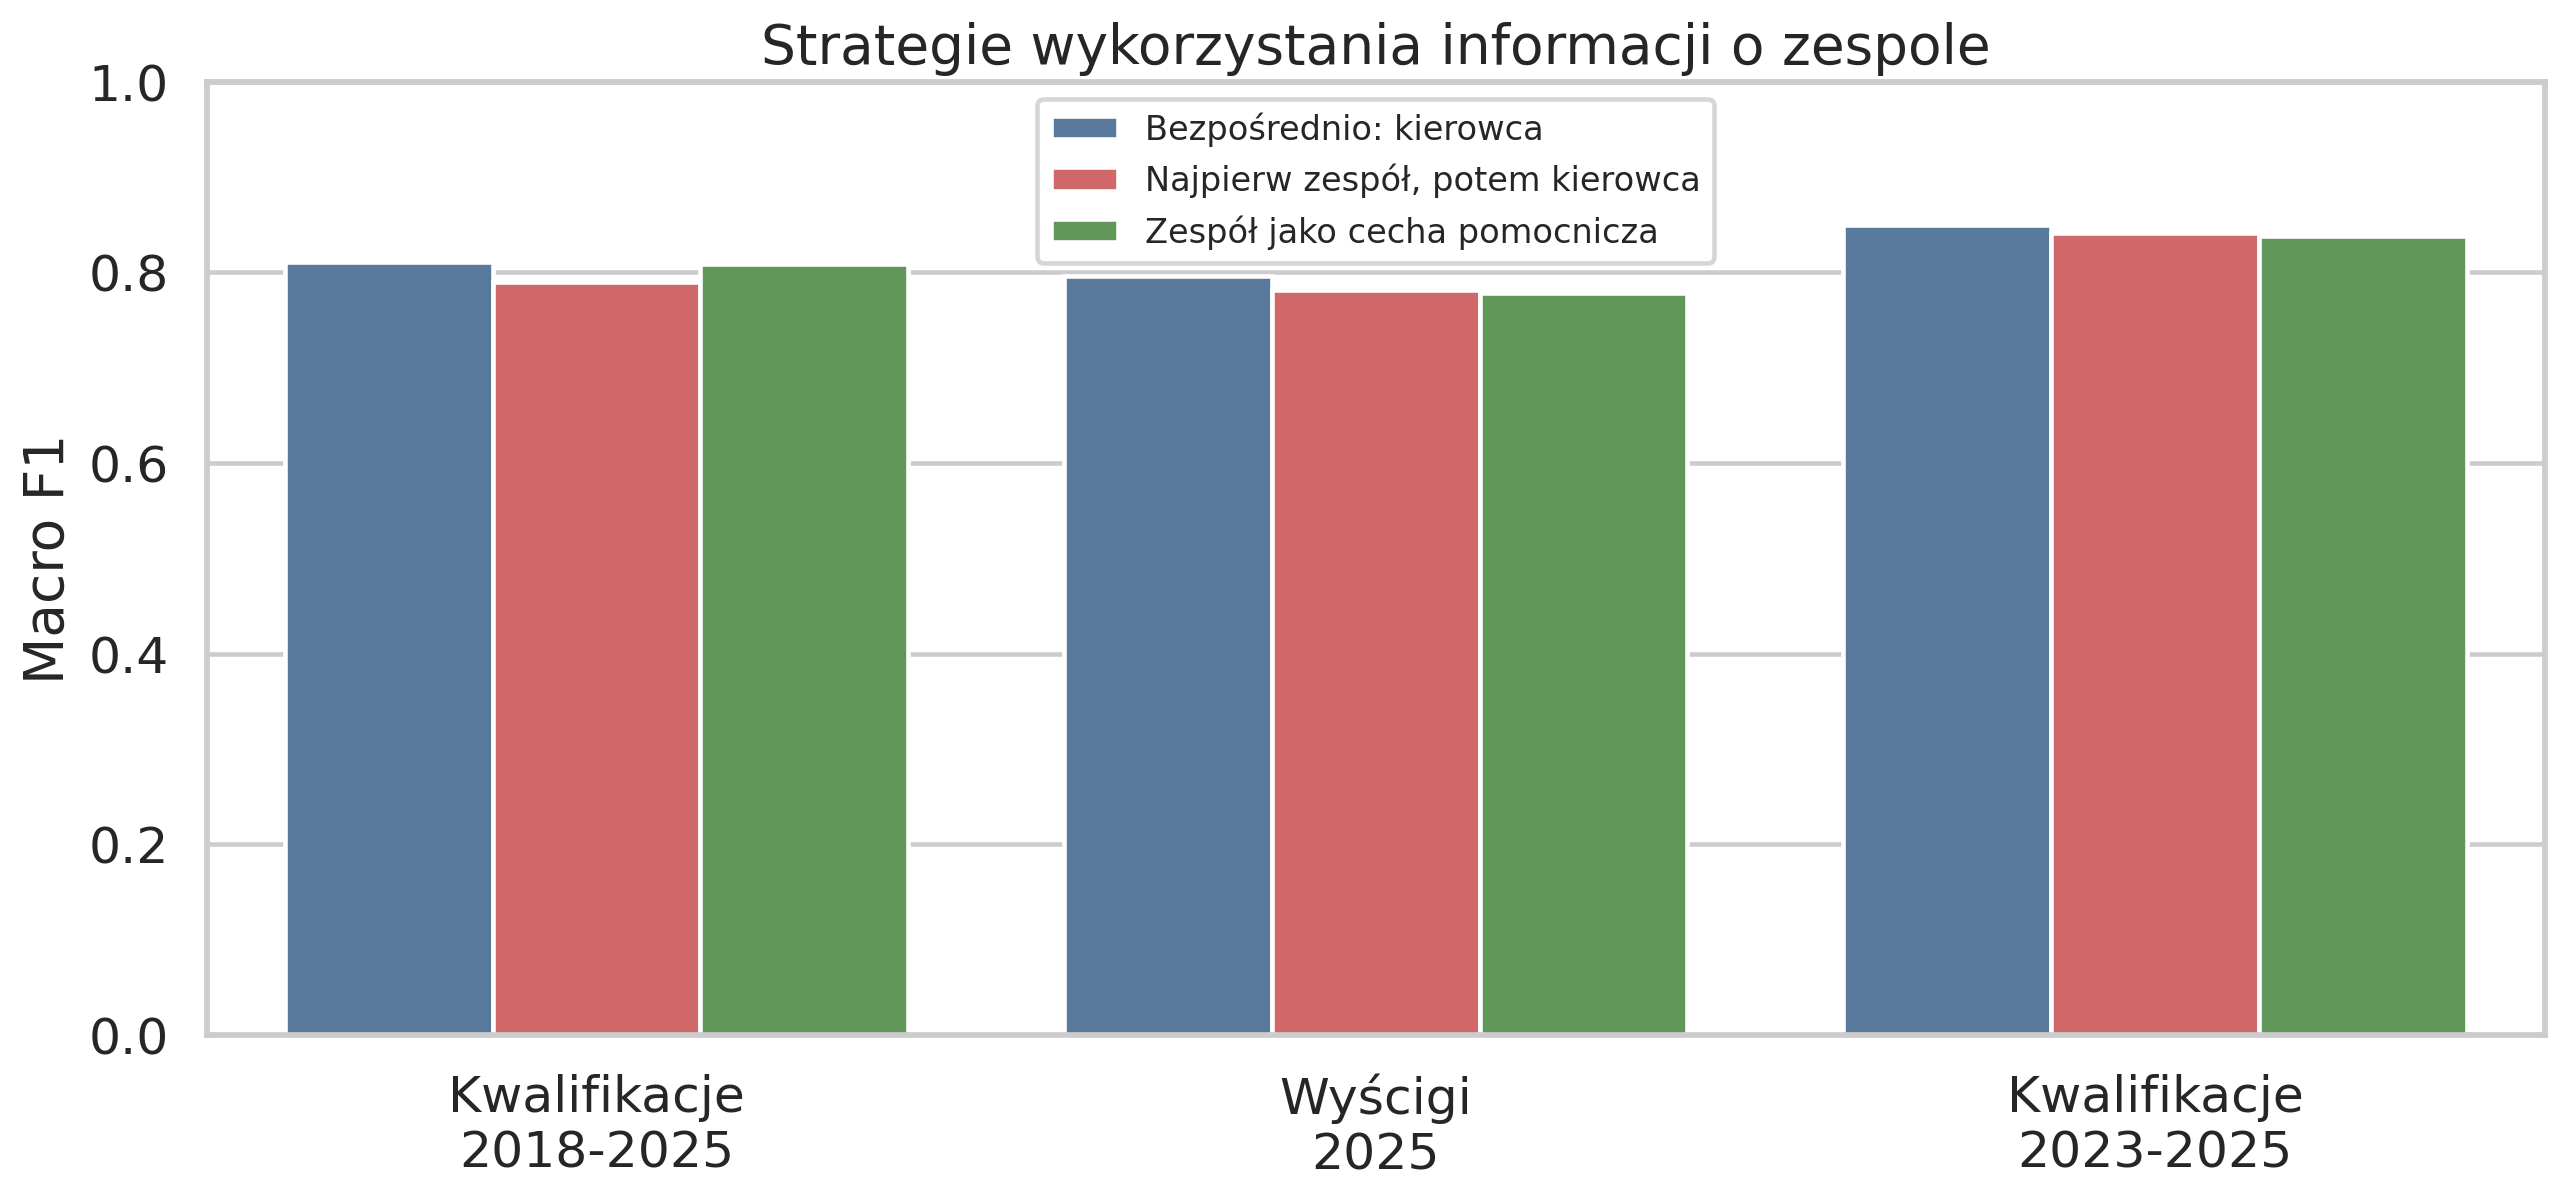
\includegraphics[width=0.90\textwidth]{08_hierarchical_team_aware_comparison.png}
\caption{Porównanie strategii wykorzystania informacji o zespole.}
\label{fig:team-aware}
\end{figure}
\FloatBarrier

Modele wykorzystujące informację o zespole dawały nierówne wyniki w bezpośredniej predykcji kierowcy. Predykcja zespołu pełni więc przede wszystkim funkcję analizy kontrolnej i interpretacyjnej, a rola finalnej ścieżki modelowania kierowcy pozostaje ograniczona.

\begin{table}[H]
\centering
\small
\begin{tabular}{lccc}
\toprule
Setup & Model bezpośredni & Model hierarchiczny & Model team-aware \\
\midrule
Kwalifikacje 2023--2025 & 0.8451 & 0.8411 & 0.8381 \\
Kwalifikacje 2018--2025 & 0.8059 & 0.7890 & 0.8086 \\
Wyścigi 2025 & 0.7965 & 0.7820 & 0.7786 \\
\bottomrule
\end{tabular}
\caption{Porównanie macro F1 dla regresji logistycznej: model bezpośredni, hierarchiczny i team-aware.}
\label{tab:hierarchical-team-aware}
\end{table}

Z tabeli~\ref{tab:hierarchical-team-aware} wynika, że predykcja zespołu jako etap pomocniczy działała nierówno. W długim setupie kwalifikacyjnym wariant team-aware minimalnie poprawił regresję logistyczną, a w pozostałych setupach pogarszał wynik. Analiza zespołowa pełni więc funkcję kontroli biasu i narzędzia interpretacyjnego. Jako finalna metoda identyfikacji kierowcy okazała się mniej stabilna od podejścia bezpośredniego.

\section{Test w tym samym zespole}

Najważniejszym testem kontrolnym jest rozróżnianie kierowców w tym samym zespole. Jeżeli model potrafi rozróżnić kierowców jadących tym samym samochodem, to sygnał kierowcy nie może być wyjaśniony wyłącznie charakterystyką zespołu.

\begin{table}[H]
\centering
\small
\begin{tabular}{lccc}
\toprule
Przypadek & Liczba okrążeń & Kierowcy & Macro F1 \\
\midrule
Ferrari, kwalifikacje 2023--2024 & 87 & LEC vs SAI & 0.8612 \\
Ferrari, wyścigi 2025 & 1742 & HAM vs LEC & 0.8820 \\
Ferrari, kwalifikacje 2018--2025 & 219 & LEC/SAI/HAM & 0.7463 \\
\bottomrule
\end{tabular}
\caption{Testy rozróżniania kierowców w tym samym zespole.}
\label{tab:same-team-tests}
\end{table}

\begin{figure}[H]
\centering
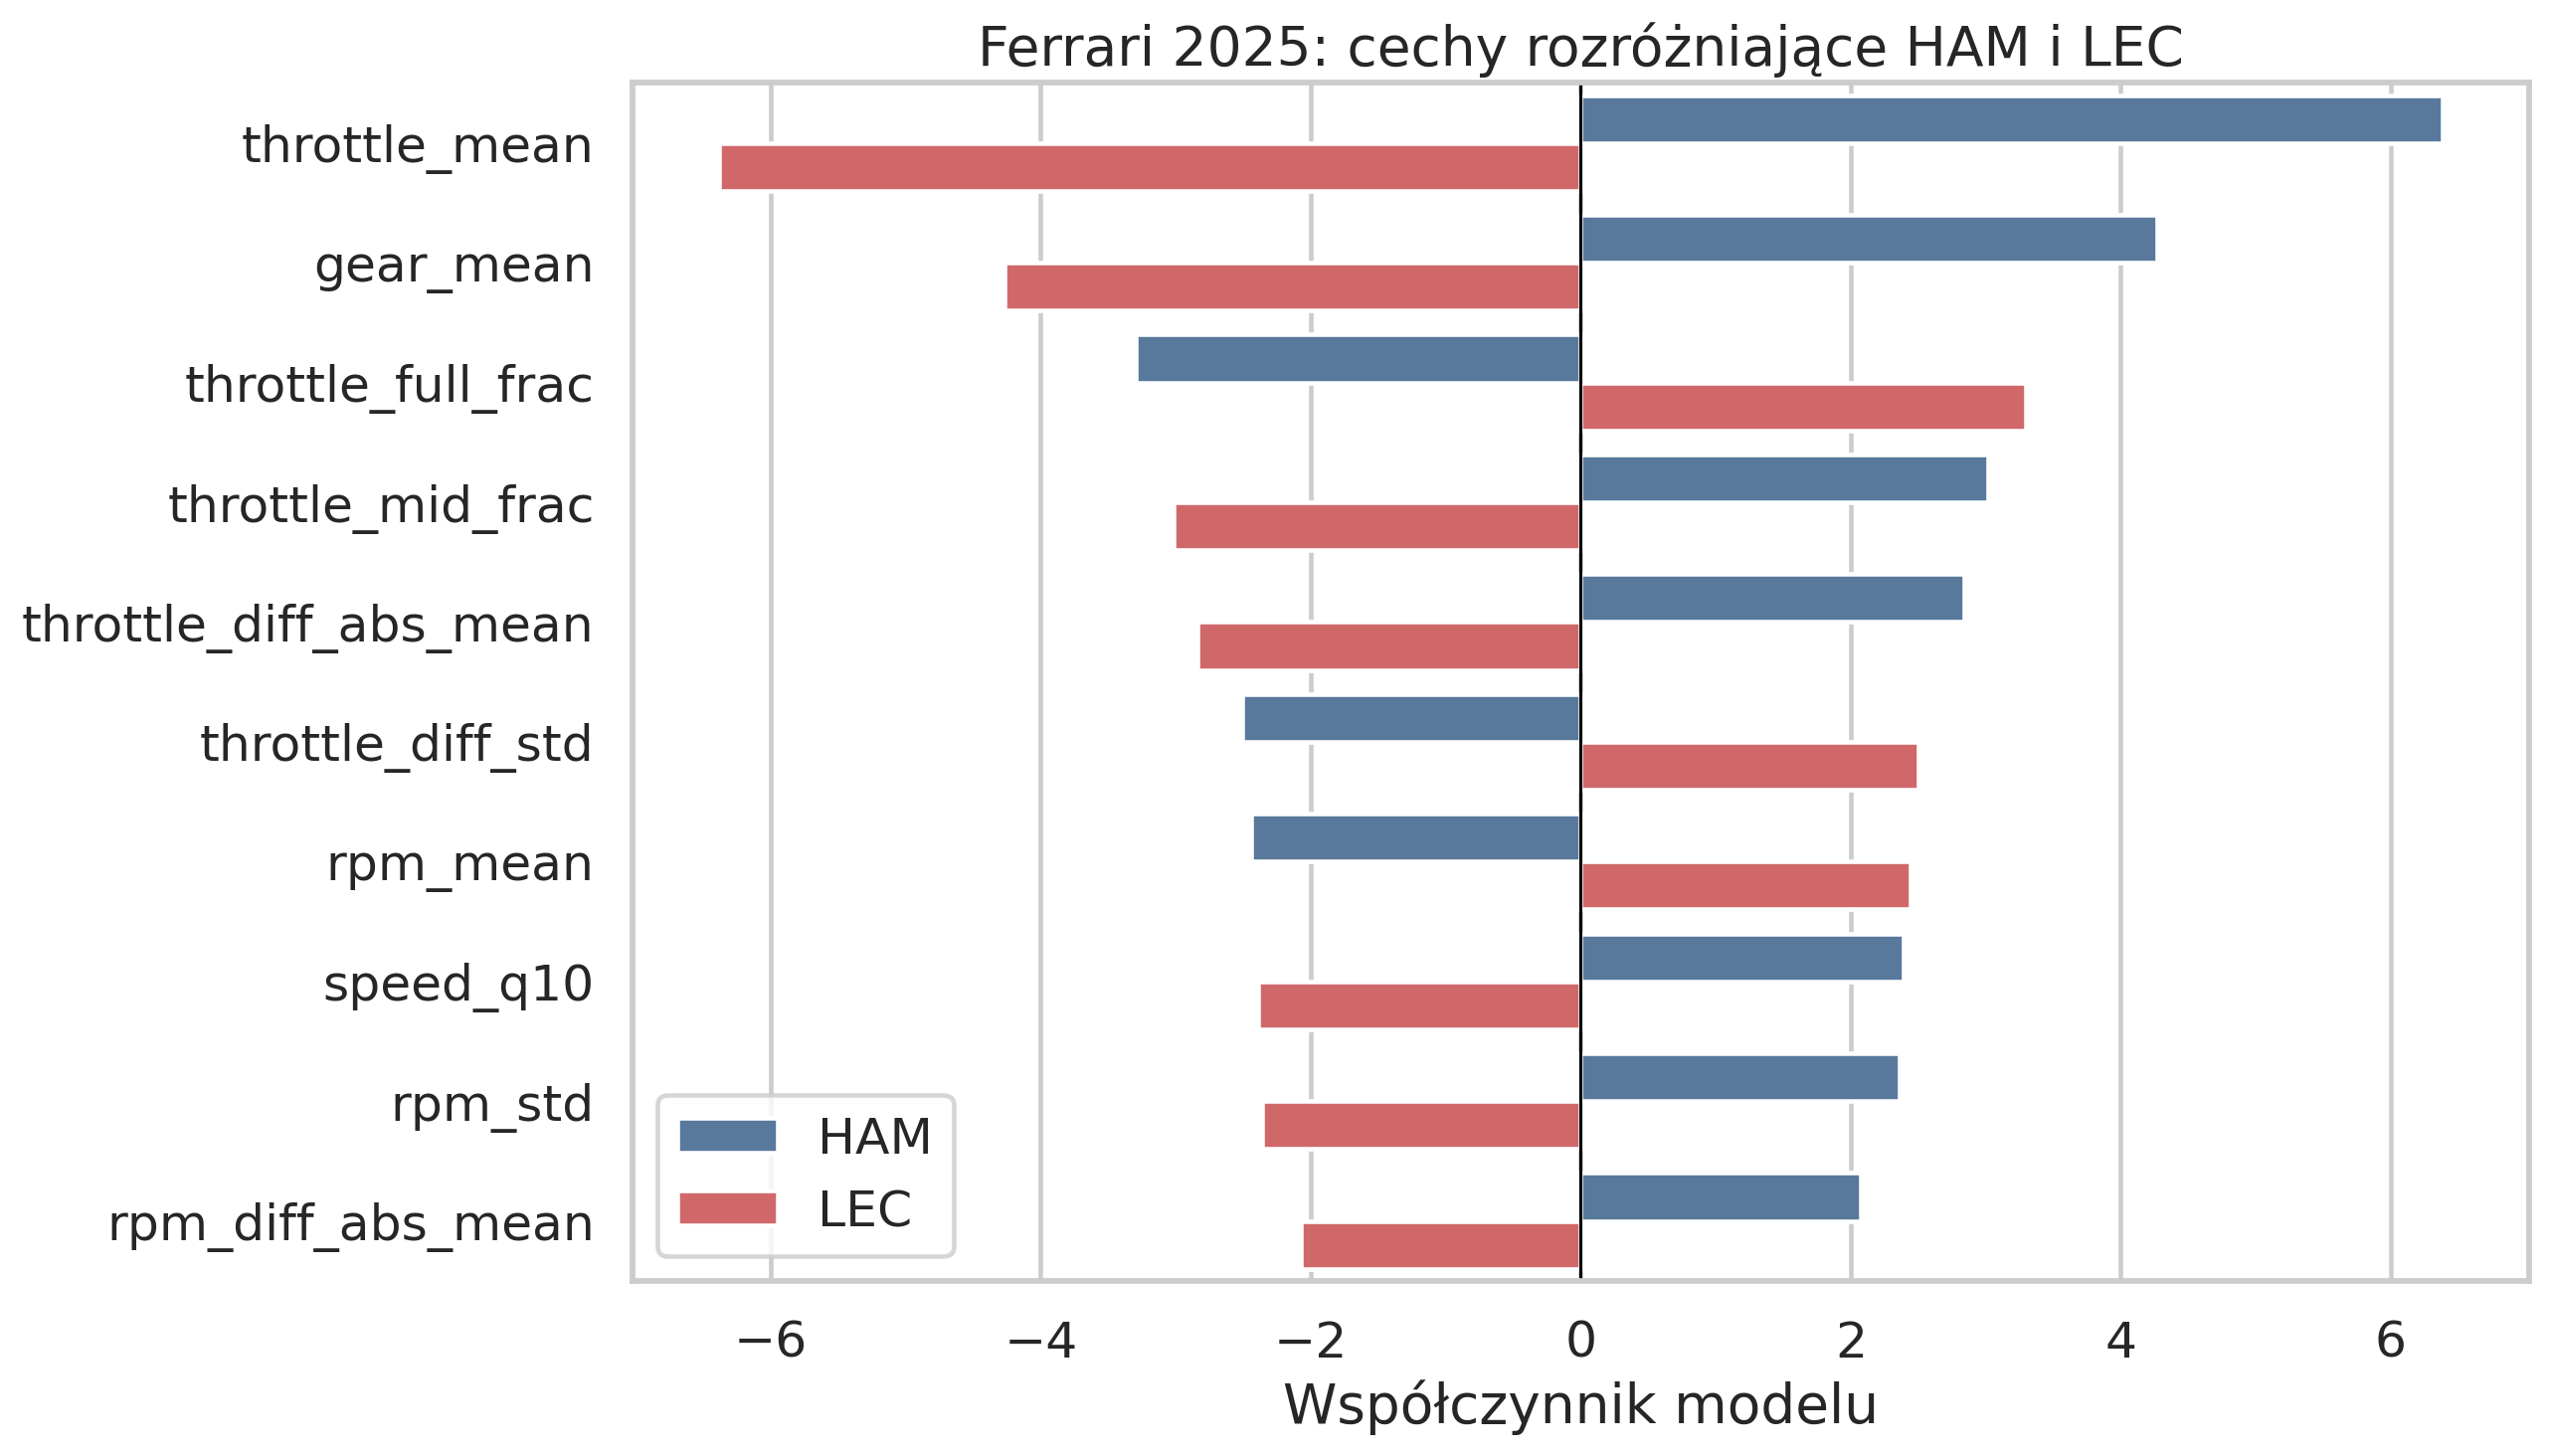
\includegraphics[width=0.90\textwidth]{09_same_team_ham_lec_feature_importance.png}
\caption{Ferrari 2025: cechy rozróżniające Hamiltona i Leclerca.}
\label{fig:same-team}
\end{figure}

Przykład Ferrari 2025 pokazuje, że model znajduje różnice między Hamiltonem i Leclerkiem mimo jazdy w tym samym zespole. Wśród ważnych cech pojawiały się między innymi cechy przepustnicy, średniego biegu, dynamiki gazu, prędkości oraz obrotów. Jest to istotny argument, że w telemetrii pozostaje indywidualny sygnał kierowcy, nawet jeżeli samochód i zespół mają własny wyraźny wpływ na dane.

Taki test jest odpowiednikiem kontroli zmiennej zakłócającej. Skoro samochód i zespół mogą wpływać na telemetrię, rozróżnianie kierowców w tym samym zespole jest silniejszym argumentem niż sama klasyfikacja kierowców z różnych zespołów. W tym sensie wyniki są zgodne z pracami o identyfikacji kierowcy z danych pojazdu i dodają kontrolę specyficzną dla Formuły 1.

\section{Kontrola toru, sezonu i ery regulacyjnej}

Na wynik klasyfikacji mogą wpływać także inne czynniki kontekstowe, takie jak tor, sezon, generacja samochodu, regulacje techniczne, pogoda, opony oraz sposób próbkowania danych. Dlatego klasyczna walidacja grupowana po sesjach została uzupełniona testami, w których całe konteksty pozostawiano poza treningiem.

W testach leave-one-context-out model trenowano na wszystkich kontekstach poza jednym, a następnie sprawdzano go na pominiętym kontekście. Dla kwalifikacji analizowano wariant leave-one-season oraz leave-one-event, a dla wyścigów leave-one-event. Dodatkowo dla długiego setupu kwalifikacyjnego wykonano test cross-era, w którym trenowano model na sezonach 2018--2021 i testowano na 2022--2025 oraz odwrotnie. Ten podział jest szczególnie ważny, ponieważ sezon 2022 oznacza istotną zmianę regulacji technicznych.

\begin{table}[H]
\centering
\small
\begin{tabular}{lccc}
\toprule
Setup & Kontrola & Średni macro F1 & Najsłabszy kontekst \\
\midrule
Kwalifikacje 2023--2025 & leave-one-season & 0.8220 $\pm$ 0.1356 & 0.6673 \\
Kwalifikacje 2023--2025 & leave-one-event & 0.8351 $\pm$ 0.1261 & 0.4667 \\
Kwalifikacje 2018--2025 & leave-one-season & 0.7477 $\pm$ 0.1808 & 0.3762 \\
Kwalifikacje 2018--2025 & leave-one-event & 0.7386 $\pm$ 0.1534 & 0.4600 \\
Wyścigi 2025 & leave-one-event & 0.7881 $\pm$ 0.1492 & 0.3976 \\
\bottomrule
\end{tabular}
\caption{Wyniki kontroli kontekstowych dla regresji logistycznej.}
\label{tab:context-control}
\end{table}

Wyniki z tabeli~\ref{tab:context-control} są niższe i bardziej zmienne niż standardowa walidacja grupowana. Taki spadek jest oczekiwany, ponieważ model testowany na niewidzianym torze albo sezonie traci część informacji charakterystycznej dla znanych warunków. Średnie wyniki pozostają jednak wyraźnie powyżej poziomu losowego dla pięciu kierowców. Oznacza to, że klasyfikator zachowuje część zdolności rozpoznawania kierowcy również poza znanym kontekstem toru lub sezonu.

Najtrudniejszy okazał się podział między erami. W długim setupie kwalifikacyjnym trening na sezonach 2018--2021 i test na 2022--2025 dał 0.5644 macro F1, a trening na 2022--2025 i test na 2018--2021 dał 0.5803. Tak duży spadek względem wyniku 0.8267 w standardowej walidacji potwierdza, że zmiana generacji samochodów i regulacji jest silnym czynnikiem zakłócającym. Wnioski o stylu kierowcy wymagają więc ostrożności, ponieważ telemetria zawiera indywidualny sygnał kierowcy spleciony z samochodem, torem i epoką regulacyjną.

Warto doprecyzować zakres tych kontroli. Test leave-one-event pomija pojedyncze wydarzenie (weekend), ale nie jest pełnym leave-one-track-out: ten sam tor może pojawić się w innych sezonach i nadal trafić do zbioru treningowego. Część pozostałych czynników kontekstowych kontrolowano nie przez wydzielanie, lecz przez filtrowanie danych: warunki mokre wykluczono, ograniczając analizę do suchych sesji, a wpływ stintu i degradacji opon ograniczono filtrem odstępstwa od lokalnej mediany stintu. Bardziej rygorystyczna kontrola, w tym ścisły leave-one-track-out (usunięcie wszystkich wizyt na danym torze) oraz jawne uwzględnienie opon i sposobu próbkowania telemetrii, pozostaje naturalnym rozszerzeniem analizy.

\chapter{Badanie 3: Stabilność stylu po zmianie zespołu}

\section{Motywacja}

Trzecie badanie rozszerza wcześniejsze wyniki. Skoro model potrafi rozpoznać kierowcę, a zespół wpływa na sygnał, naturalnym pytaniem jest to, czy elementy stylu kierowcy są częściowo stabilne po zmianie samochodu.

Analiza skupia się na tym, czy po zmianie zespołu wybrane profile telemetryczne kierowcy pozostają do siebie podobne. Jest to praktyczny sposób sprawdzenia, które elementy stylu mogą być względnie stabilne mimo zmiany samochodu.

\section{Metoda}

Porównano kierowców, którzy w analizowanym okresie zmieniali zespoły. Cechy były normalizowane względem sesji, aby ograniczyć wpływ toru i warunków. Następnie dla każdego kierowcy porównano profile \emph{kierowca--zespół}.

W głównej części pokazano wybrane przypadki, natomiast pełne wyniki powinny zostać umieszczone w dodatku lub repozytorium. Ogranicza to ryzyko wybierania wyłącznie przykładów pasujących do tezy.

Miarą podobieństwa profili była mediana podobieństwa cosinusowego między profilami \emph{kierowca--zespół}. Wartości tej miary należy odczytywać względem punktu odniesienia. Dla par różnych kierowców mediana podobieństwa wyniosła -0.0998, górny kwartyl 0.1965, a 90. percentyl 0.4648. Dla par tego samego kierowcy jeżdżącego w różnych zespołach średnia wyniosła 0.4921, a typowy zakres międzykwartylowy 0.3942--0.6426. Dzięki temu wartości z tabeli~\ref{tab:transfer-cases} mają skalę interpretacyjną: wyniki Ocona, Gasly'ego i Alonso znajdują się wyraźnie powyżej typowego podobieństwa różnych kierowców, a wyniki Sainza i Bottasa są znacznie słabsze. Należy przy tym pamiętać, że baseline podano jako średnią i rozstęp międzykwartylowy po wszystkich parach, podczas gdy tabela~\ref{tab:transfer-cases} zawiera mediany wyznaczone osobno dla każdego kierowcy; obie miary opisują tę samą wielkość, lecz na różnym poziomie agregacji.

\section{Wyniki stabilności stylu}

Zbiorcze porównanie stabilności profilu stylu między zespołami przedstawiono na rysunku~\ref{fig:transfer-stability}.

\begin{figure}[H]
\centering
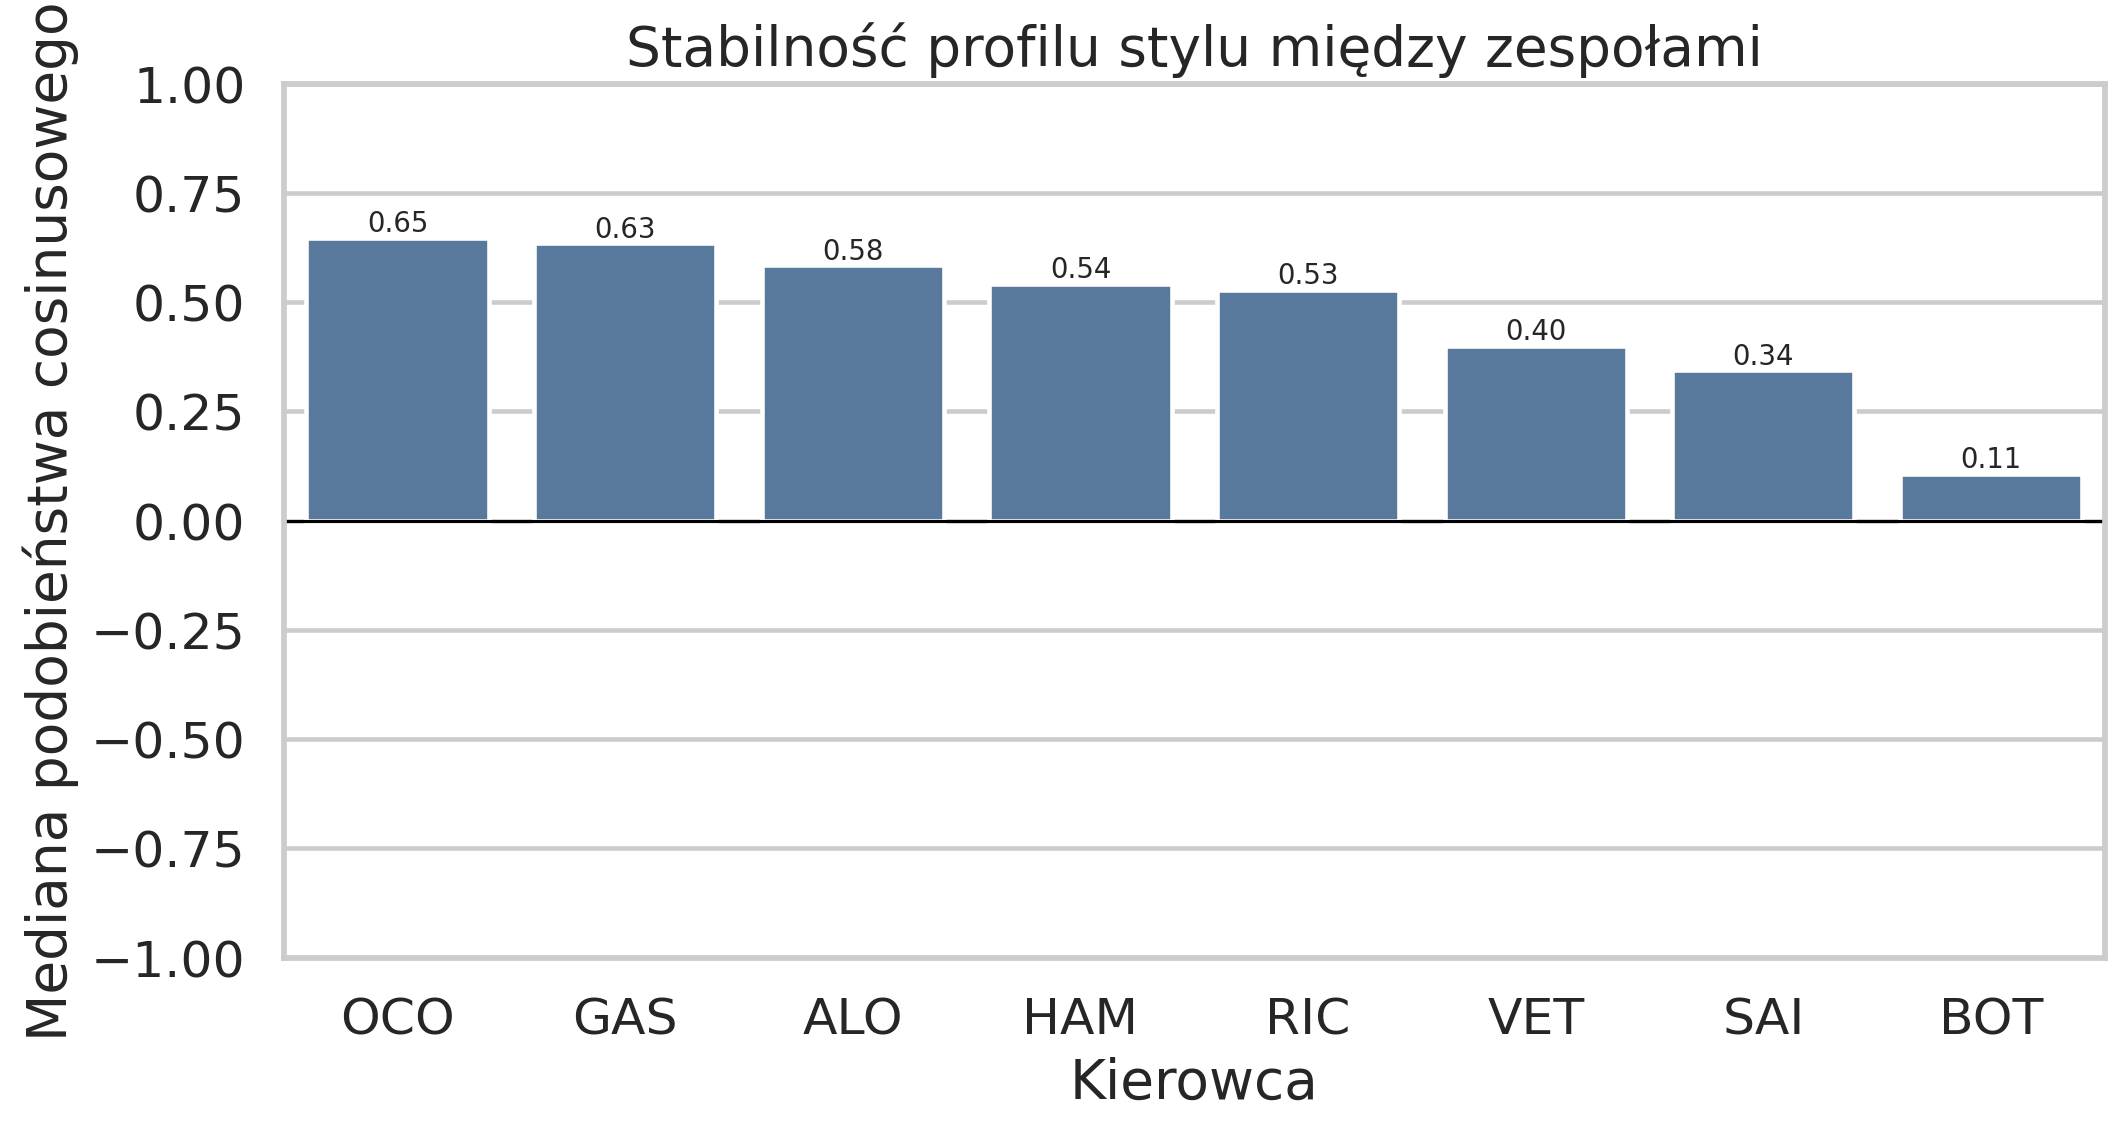
\includegraphics[width=0.90\textwidth]{19_driver_style_transfer_stability_summary.png}
\caption{Stabilność profilu stylu między zespołami dla kierowców zmieniających zespół.}
\label{fig:transfer-stability}
\end{figure}

Rysunek pokazuje zróżnicowaną stabilność profilu. U części kierowców podobieństwo między zespołami pozostaje wyraźne, a u innych jest znacznie słabsze.

\begin{table}[H]
\centering
\small
\begin{tabular}{lccc}
\toprule
Kierowca & Liczba par zespołów & Mediana podobieństwa & Interpretacja \\
\midrule
OCO & 10 & 0.648 & mocny przykład stabilności \\
GAS & 6 & 0.634 & mocny przykład stabilności \\
ALO & 3 & 0.584 & mocny przykład stabilności \\
HAM & 1 & 0.542 & pojedyncza para zespołów \\
RIC & 10 & 0.528 & częściowy przykład \\
VET & 1 & 0.400 & pojedyncza para zespołów \\
SAI & 6 & 0.345 & kontrprzykład \\
BOT & 3 & 0.107 & kontrprzykład \\
\bottomrule
\end{tabular}
\caption{Wybrane przypadki stabilności stylu po zmianie zespołu.}
\label{tab:transfer-cases}
\end{table}

\begin{figure}[H]
\centering
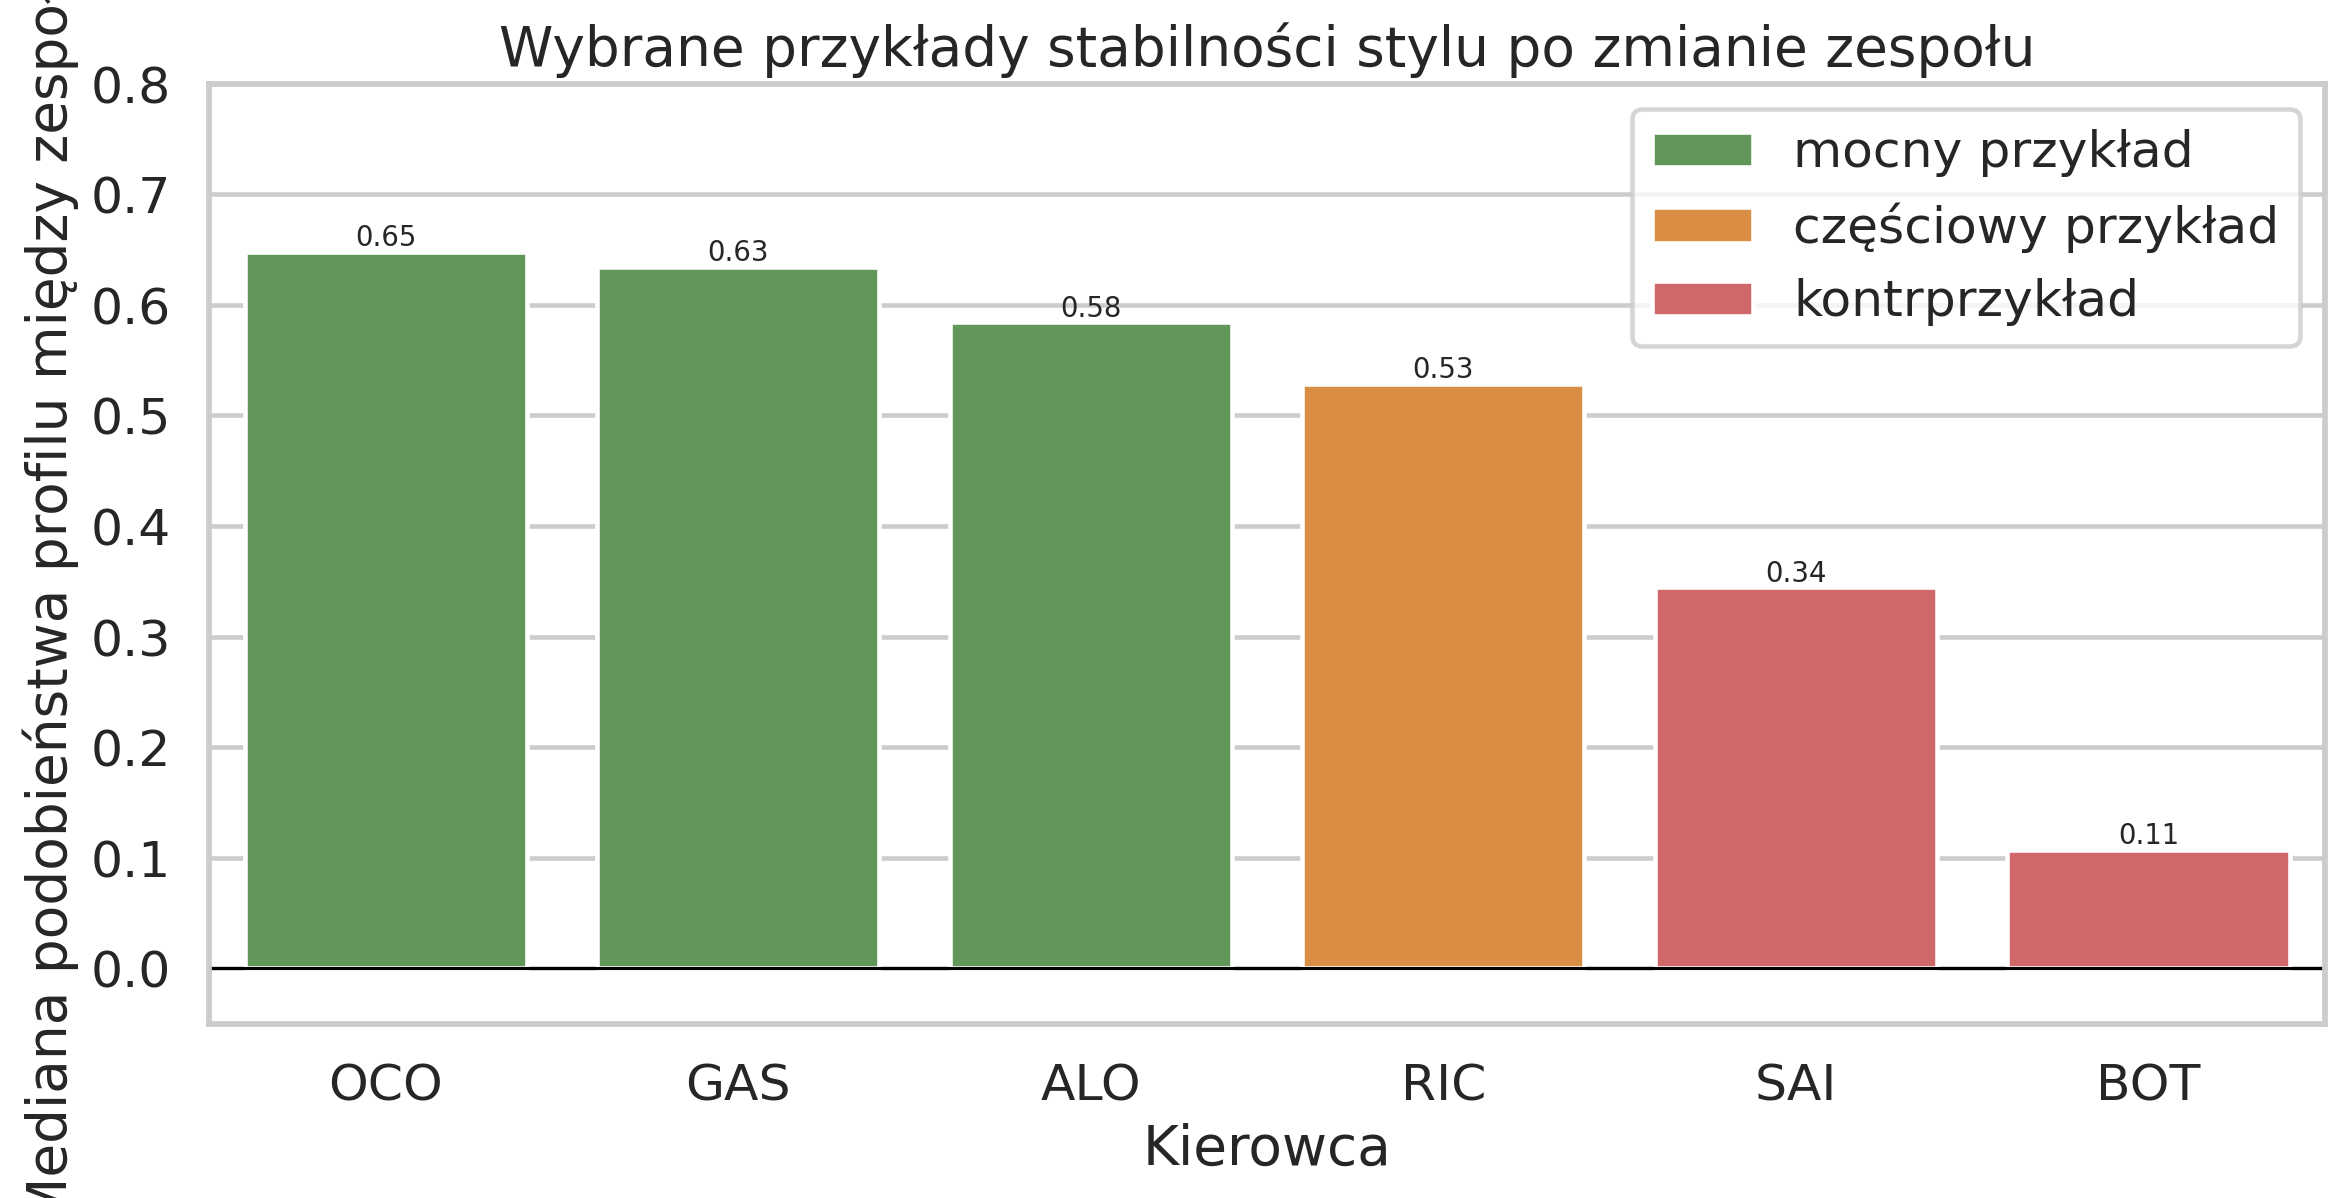
\includegraphics[width=0.90\textwidth]{23_selected_driver_transfer_case_studies.png}
\caption{Wybrane przykłady stabilności i niestabilności stylu po zmianie zespołu.}
\label{fig:selected-transfer}
\end{figure}
\FloatBarrier

Wyniki sugerują, że u części kierowców profil stylu pozostaje częściowo stabilny po zmianie zespołu. Najmocniejsze przykłady w tej analizie to Ocon, Gasly i Alonso. Ricciardo jest przypadkiem częściowym, z podobieństwem widocznym tylko dla części profili między zespołami. Sainz i Bottas pokazują natomiast, że samochód i kontekst mogą znacząco zmienić profil telemetryczny. Hamilton i Vettel opierają się w tej analizie tylko na jednej zmianie zespołu, dlatego ich wyniki (odpowiednio 0.542 i 0.400) traktowano jako mniej pewne niż przypadki wsparte wieloma parami zespołów.

\section{Synteza wyników}

Powiązanie kolejnych etapów analizy przedstawiono na rysunku~\ref{fig:research-arc}.

\begin{figure}[H]
\centering
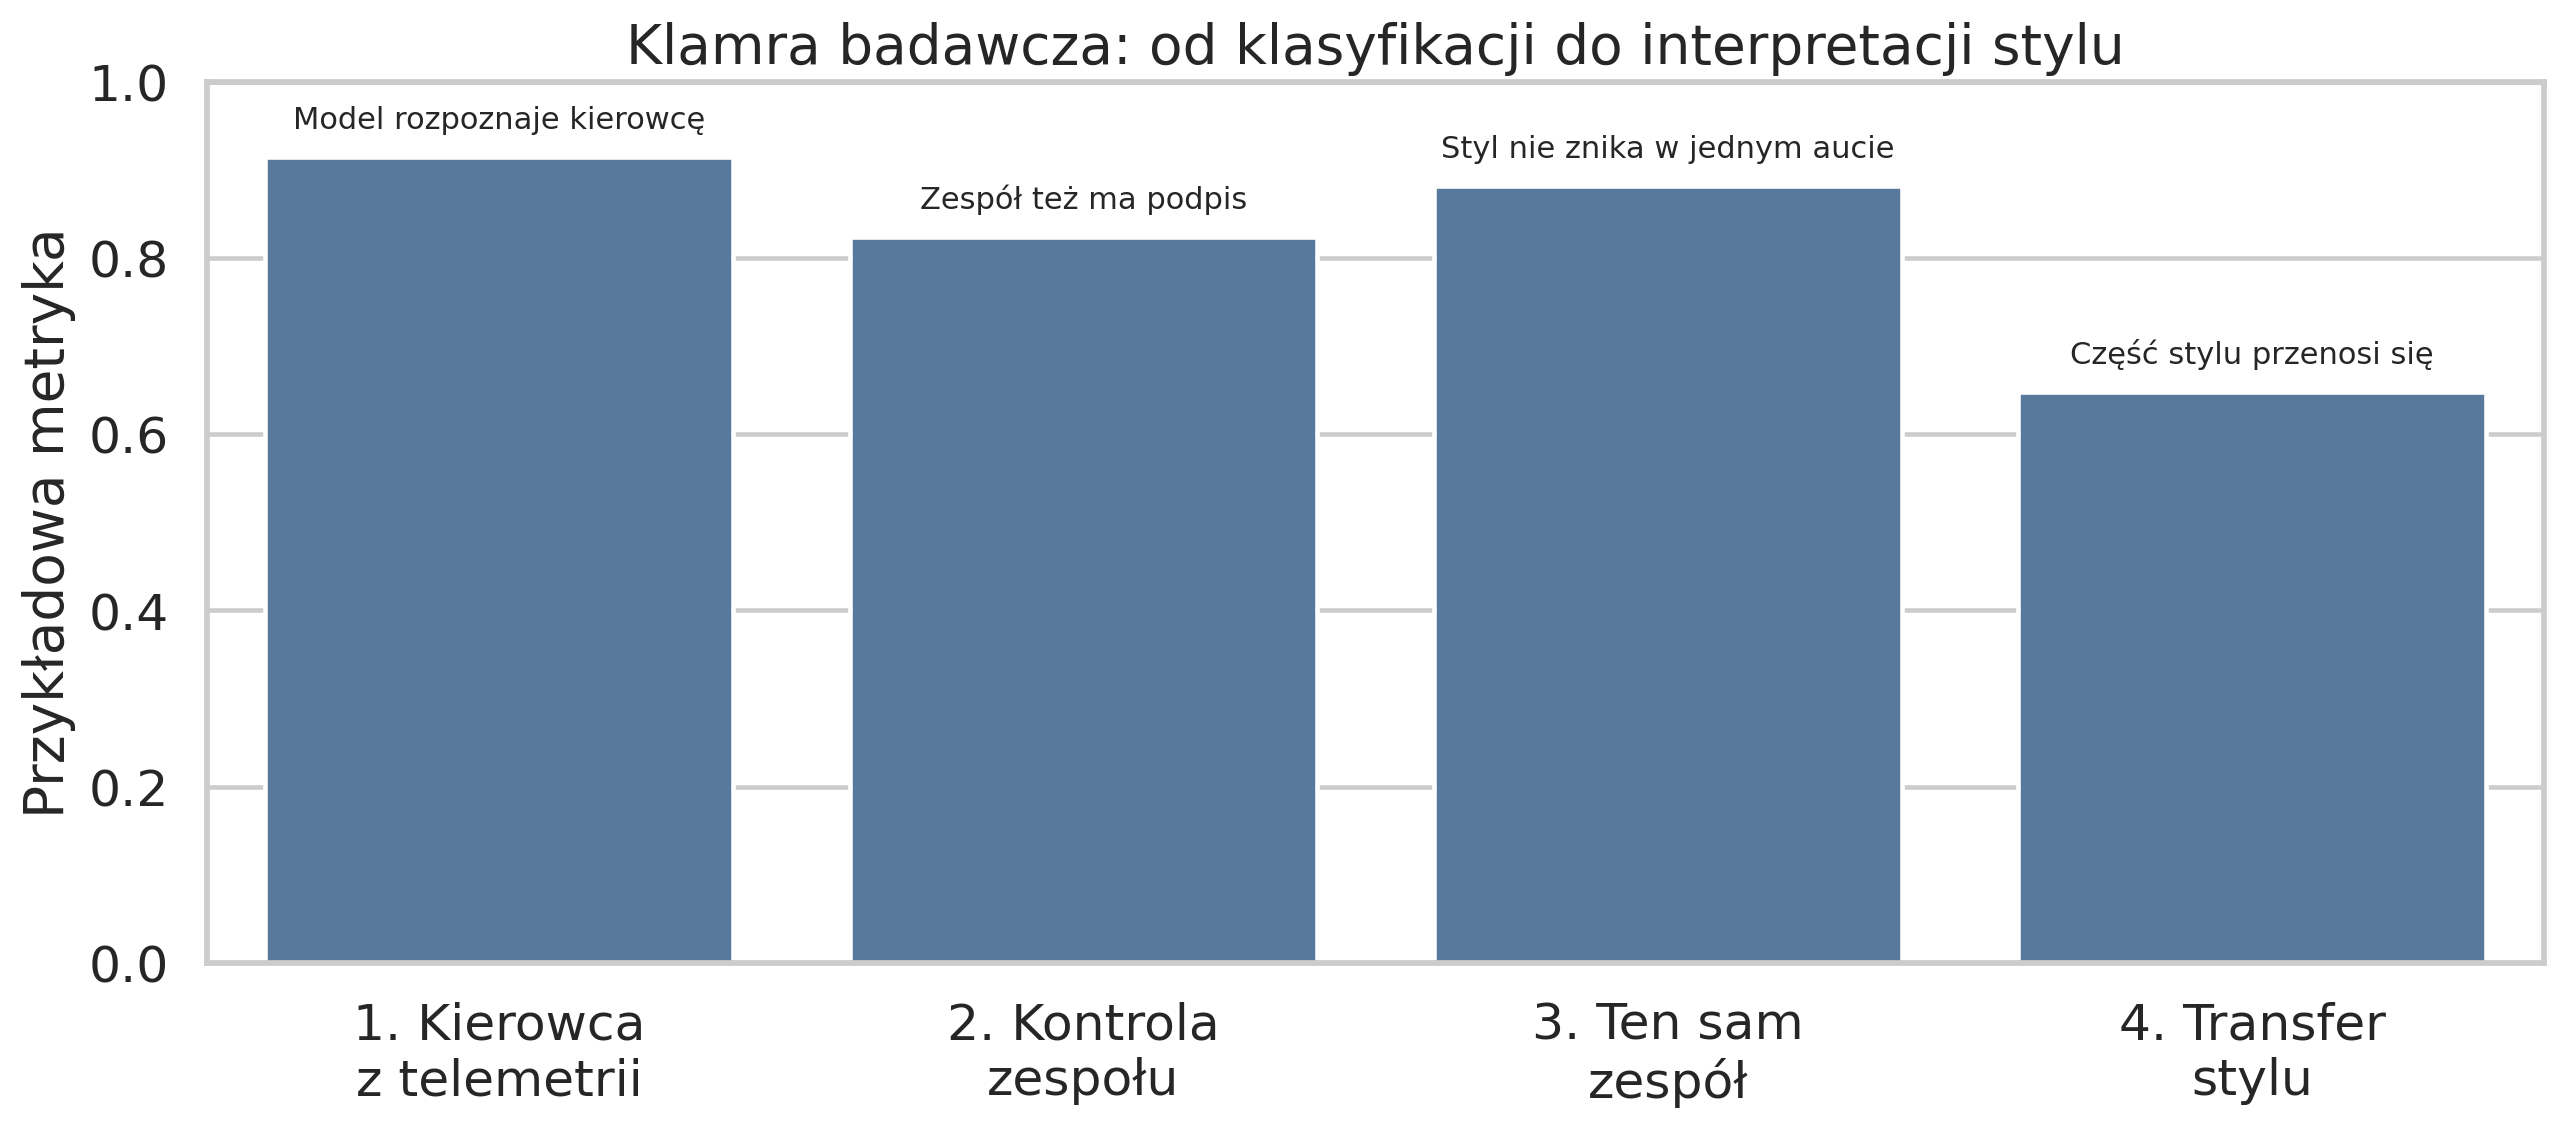
\includegraphics[width=0.90\textwidth]{22_thesis_research_arc.png}
\caption{Proces badawczy: od klasyfikacji do interpretacji stylu.}
\label{fig:research-arc}
\end{figure}

Proces badawczy prowadzi od klasyfikacji do interpretacji:

\begin{enumerate}
    \item modele potrafią rozpoznać kierowcę na podstawie telemetrii;
    \item zespół również ma podpis telemetryczny, więc konieczna jest kontrola biasu;
    \item testy w tym samym zespole pokazują, że indywidualny sygnał kierowcy nie znika;
    \item wybrane przypadki transferu między zespołami sugerują, że część stylu może być stabilna mimo zmiany samochodu.
\end{enumerate}

\chapter{Podsumowanie i dalsze prace}

Praca pokazuje, że identyfikacja kierowcy Formuły 1 na podstawie telemetrii jest możliwa. Modele osiągały wyniki wyraźnie lepsze od losowych we wszystkich trzech setupach eksperymentalnych, a najlepsze rezultaty uzyskiwały modele sekwencyjne i hybrydowe. Regresja logistyczna pozostała natomiast ważnym punktem odniesienia, ponieważ łączyła klasyfikację kierowców z interpretacją cech związanych z decyzją modelu.

Uzyskane wyniki pokazują, że telemetria zawiera informacje opisujące sposób pokonywania okrążenia. Różnice między kierowcami były widoczne zarówno w ręcznie zdefiniowanych cechach, jak i w przebiegach sekwencyjnych. Modele wykorzystywały między innymi informacje związane z prędkością, pracą gazu, hamowaniem, biegami, obrotami silnika i dynamiką sygnałów. Oznacza to, że końcowy czas okrążenia nie wyczerpuje opisu jazdy kierowcy.

Ważnym rozszerzeniem była analiza wpływu zespołu i samochodu. Zespół również ma własny profil telemetryczny, dlatego klasyfikacja kierowcy wymaga uwzględnienia samochodu. Testy w obrębie tego samego zespołu oraz analiza kierowców zmieniających zespoły sugerują, że indywidualny profil kierowcy pozostaje częściowo widoczny. Styl jazdy jest więc wynikiem interakcji kierowcy, samochodu i kontekstu sesji.

Eksperymenty kontrolne pokazały też granice uogólniania. Wyniki leave-one-season, leave-one-event i cross-era były niższe od standardowej walidacji grupowanej, szczególnie po rozdzieleniu sezonów 2018--2021 i 2022--2025. Model rozpoznaje kierowcę w kontekście konkretnej telemetrii Formuły 1, a część informacji pozostaje powiązana z torem, sezonem, samochodem i erą regulacyjną.

Zakres wniosków jest ograniczony przez charakter publicznie dostępnych danych. Część obserwowanych różnic można interpretować tylko pośrednio, bez pełnego dostępu do informacji inżynierskich wykorzystywanych przez zespoły. Mimo tego dostępna telemetria okazała się wystarczająca do zbudowania spójnego procesu badawczego, raportowania niepewności wyników oraz wykonania dodatkowych kontroli ograniczających ryzyko zbyt prostej interpretacji.

\section{Możliwe dalsze kierunki}

\begin{itemize}
    \item precyzyjne wyrównanie czasowe danych samochodu i pozycji;
    \item segmentacja okrążenia na zakręty i mini-sektory;
    \item analiza stylu kierowcy tor po torze;
    \item wykorzystanie danych OpenF1 jako niezależnego źródła walidacji;
    \item budowa embeddingów stylu kierowcy z użyciem metod samonadzorowanych lub kontrastywnych;
    \item porównanie z architekturami TCN, InceptionTime oraz transformerami dla szeregów czasowych;
    \item rozszerzenie interpretowalności o SHAP, partial dependence i lokalne wyjaśnienia pojedynczych okrążeń;
    \item testy transferu modeli między erami regulacyjnymi i między seriami wyścigowymi;
    \item dashboard do porównywania kierowców i zespołów;
    \item analiza transferu kierowcy między zespołami na większej liczbie sezonów.
\end{itemize}

\cleardoublepage
\printbibliography[heading=bibintoc,title={Literatura}]

% Opcjonalnie, jeżeli promotor/uczelnia tego wymaga:
% \listoffigures
% \listoftables

\end{document}